\chapter{Zaimplementowane elementy maszyny wirtualnej}
\label{cha:maszyna}

Maszyna wirtualna jest warstwą abstrakcji uruchamianą pod kontrolą pewnego systemu operacyjnego.
Powinna ona emulować fizyczny procesor w taki sam sposób niezależnie od systemu operacyjnego czy fizycznej architektury na jakiej została uruchomiona.
Dzięki temu możliwe jest uruchomienie tego samego kodu, nazywanego kodem pośrednim, przystosowanego do architektury maszyny wirtualnej, pod kontrolą różnych systemów operacyjnych i na różnych architekturach sprzętowych.

Wśród funkcjonalności wirtualnego procesa, które powinna implementować maszyna wirtualna dowolnego języka można wymienić:
\begin{itemize}
\item struktury danych, przy pomocy których opisane są instrukcje i ich argumenty;
\item stos, wykorzystywany do wywołań funkcji;
\item wskaźnik kolejnej instrukcji do wykonania;
\item interpreter kodu pośredniego, pobierający kolejną instrukcję do wykonania, dekodujący jej argumenty i wykonujący ją.
\end{itemize}

W rozdziale wymieniono elementy maszyny wirtualnej Erlanga, które zaimplementowano w pracy, tak aby powyższy zbiór funkcjonalności zapewniał możliwość wykonywania kodu modułów skompilowanych przy użyciu kompilatora Erlanga w wersji R16.
Opis poszczególnych elementów zawiera wyjaśnienie ich sposobu działania, ich roli w maszynie wirtualnej, a także porównania
funkcjonalności do maszyny wirtualnej BEAM.

Wszystkie opisywane funkcjonalności zostały zaimplementowane w języku C, w oparciu o kod źródłowy maszyny wirtualnej BEAM, który opublikowany jest na licencji \emph{Erlang Public License} \cite{epl}.

%---------------------------------------------------------------------------
\section{Moduł ładujący kod (\emph{loader})}
\label{sec:maszynaLoader}

Moduł opisany w niniejszym podrozdziale został zaimplementowany w pliku źródłowym \texttt{beam\_load.c}.

Podstawowym zadaniem \emph{loadera} jest wykonanie zestawu operacji po których będzie możliwe wykonanie kodu programu, zawartego w pliku będącym efektem kompilacji modułu w języku Erlang, z~poziomu interpretera kodu pośredniego w maszynie wirtualnej.
W maszynie BEAM źródłem plików binarnych może być system plików systemu operacyjnego lub inny węzeł Erlanga znajdujący się w tym samym klastrze. Aby pliki te mogły być wykonywane na maszynie zaimplementowanej w ramach pracy, która nie obsługuje ani systemu plików ani protokołu klastrowania, muszą one ulec przetworzeniu i zostać wkompilowane w kod maszyny wirtualnej. Dokonywane jest to za pomocą narzędzia opisanego w~dodatku \ref{cha:builder}.

Zawartość pliku, który poddawany jest przetwarzaniu w module została szczegółowo opisana w dodatku \ref{cha:erlangKompilacja}, który ze względu na brak oficjalnej dokumentacji powstał na potrzeby niniejszej pracy.

Aby możliwe było wykonywanie kodu pośredniego przez maszynę wirtualną, konieczne jest wykonanie następujących kroków:
\begin{itemize}
\item załadowanie lokalnej tablicy atomów (fragment \texttt{Atom}) do globalnej tablicy atomów (por. \ref{sub:maszynaTablicaAtomow});
\item załadowanie lokalnej tablicy eksportowanych funkcji (fragment \texttt{ExpT}) do jej globalnego odpowiednika (por. \ref{sub:maszynaTablicaEksportow});
\item sparsowanie wyrażeń w postaci \emph{External Term Format}, umieszczonych we fragmencie \texttt{LitT} i~umieszczenie ich w pamięci o globalnym dostępie (globalnej stercie);
\item wyszukanie w globalnej tablicy eksportów funkcji zewnętrznych używanych przez moduł (fragment \texttt{ImpT});
\item podstawienie wyrażeń rozpoznawanych globalnie (por. \ref{sec:maszynaTypy}) za wyrażenia lokalne, opisane w podrozdziale \ref{sec:opsTypes} we fragmencie \texttt{Code}. Do rozważanych wyrażeń należą: atomy, etykiety lokalnych funkcji, odnośniki do funkcji znajdujących się w innych modułach oraz wyrażenia umieszczone na globalnej stercie;
\item podstawienie za numery operacji z sekcji \texttt{Code} (opisane w podrozdziale \ref{sec:opsOps}) wskaźników do odpowiedniej sekcji interpretera kodu maszynowego wykonującemu daną instrukcję (por. \ref{sec:maszynaInterpreter}).
\end{itemize}

\emph{Loader} maszyny wirtualnej BEAM wykonuje jeszcze jeden bardzo istotny krok, którego nie wykonuje maszyna zaimplementowana w pracy. Jest nim zastosowanie gramatyki modyfikującej w bardzo istotny sposób kod maszynowy zawarty w pliku binarnym. Gramatykę tę można znaleźć w pliku \texttt{ops.tab} w kodzie źródłowym maszyny BEAM. Wynikowy zestaw instrukcji, odpowiadający instrukcjom faktycznie interpretowanym przez BEAM, jest dużo bardziej obszerny od zestawu który może zostać wygenerowany przez kompilator. Motywacją do zmiany kodu maszynowego w~ten sposób jest m.in. optymalizacja czasu wykonania często występujących po sobie operacji. W przeciwieństwie do oryginalnej maszyny wirtualnej, interpreter zawarty w niniejszej maszynie wirtualnej dokonuje bezpośredniej interpretacji opkodów, które znajdują się w pliku binarnym z kodem pośrednim.

%---------------------------------------------------------------------------
\section{Tablice}
\label{sec:maszynaTablice}

Tablice opisane w tym podrozdziale zostały zaimplementowane w plikach \texttt{hash.c}, \texttt{index.c}, \texttt{atom.c} oraz \texttt{export.c}.

Biorąc pod uwagę modułowy charakter aplikacji napisanych w języku Erlang, maszyna wirtualna musi posiadać pewien mechanizm pozwalający na utrzymywanie globalnego stanu systemu w zależności od aktualnie załadowanych modułów.

Strukturą danych przeznaczoną do tego celu jest tablica z haszowaniem wspomagana przez tablicę indeksów. Połączenie tych dwóch struktur umożliwia wstawienie nowego elementu oraz sprawdzenie jego indeksu w czasie stałym (konieczne jest wyliczenie skrótu). W takim samym czasie (nie jest do tego jednak konieczne wyliczanie skrótu) możliwe jest znalezienie obiektu znając jego indeks. Co więcej, w~reprezentacji kodu maszynowego posługiwanie się indeksami obiektów trywializuje ich porównywanie czy pobieranie ich wartości w trakcie jego wykonywania.

Wybór takiej struktury danych ma więc charakter optymalizacyjny. W maszynie wirtualnej tablicowanymi obiektami są: atomy i eksportowane funkcje. Maszyna wirtualna BEAM dodatkowo tablicuje również moduły, gdzie przechowywane są informacje o wskaźnikach do początku kodu modułu w dwóch wersjach: nowej i starej, które mogą działać w maszynie wirtualnej niezależnie od siebie. Ponieważ jednak maszyna rozważana w pracy w obecnej fazie rozwoju nie zapewnia możliwości dynamicznego ładowania modułów, implementacja tej struktury nie było konieczne.

Na rysunku \ref{fig:atomtable} przedstawiono sposób w jaki wewnątrz maszyny wirtualnej przechowywane są stablicowane dane.  Przykład ten dotyczy dwuelementowej tablicy atomów, które były do niej wstawiane w~kolejności: \texttt{erlang}, \texttt{+}. Strzałki na diagramie reprezentują przechowywanie wskaźników na struktury atomów przez tablice: z haszowaniem i indeksów.

\begin{figure}[h]
\centerline{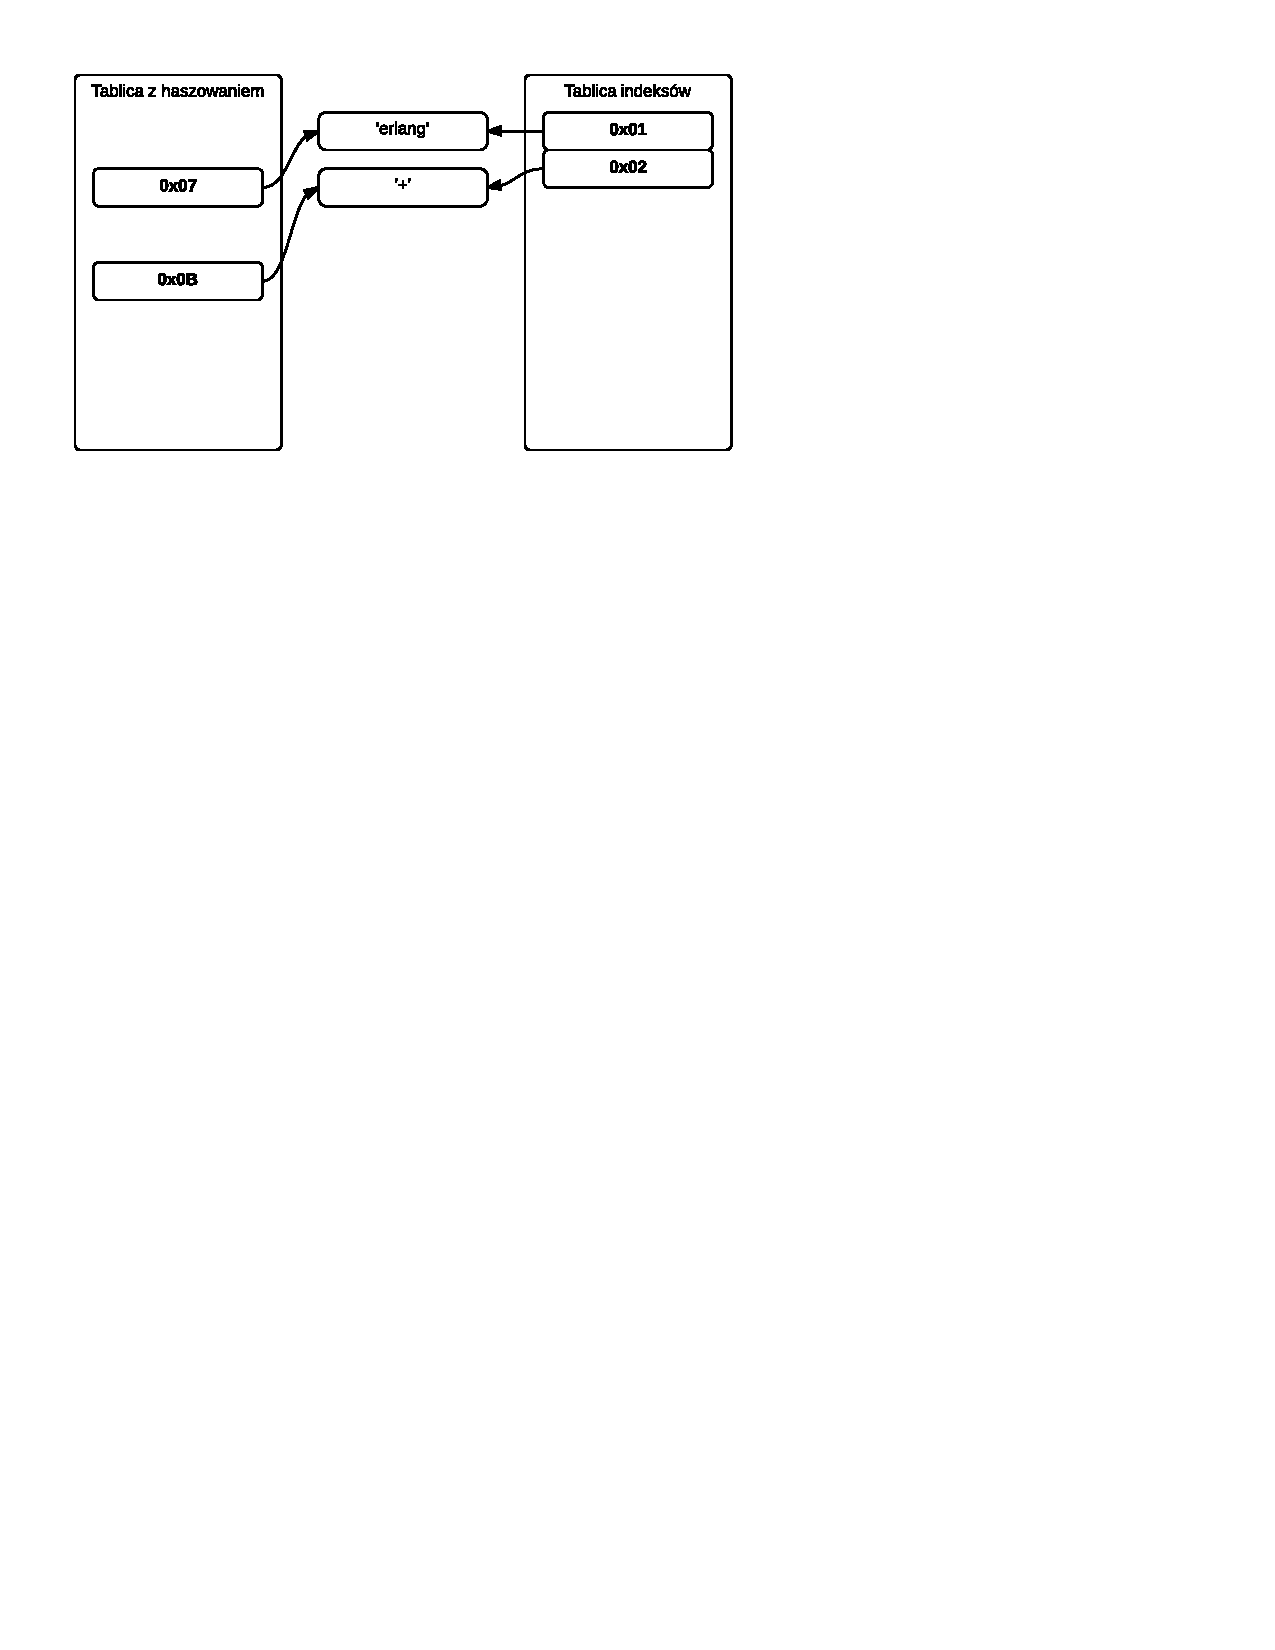
\includegraphics[scale=1, clip, trim=10mm 200mm 90mm 10mm]{atom_table}}
\caption{Przykład przechowywania danych stablicowanych danych wewnątrz maszyny wirtualnej.}
\label{fig:atomtable}
\end{figure}

W maszynie BEAM, w przypadku uruchomionych dużych systemów, powyższe struktury danych mogą zawierać bardzo dużą liczbę elementów, nawet rzędu kilkudziesięciu tysięcy. Zupełnie inaczej sytuacja wygląda w niniejszej maszynie wirtualnej ze względu na jej przeznaczenie, którym są systemy wbudowane i wynikające z tego restrykcyjne limity dostępnej pamięci RAM. Rozmiary tablic nie powinny zatem przekraczać liczby elementów wyrażonej w setkach atomów czy funkcji eksportowanych. Niemniej jednak, ze względu na możliwość uruchomienia systemu FreeRTOS na mikrokontrolerach o różnych parametrach, pozostawiono możliwość zdefiniowania maksymalnej liczby elementów, jakie mogą zostać wstawione do tablic. Zaimplementowano również mechanizmy automatycznego rozszerzania tablic wraz ze wzrostem liczby elementów, w celu optymalizacji pamięci zajmowanej przez tablice.

Ważną cechą charakterystyczną tablic w maszynie wirtualnej jest również fakt, że raz wstawionego do nich obiektu nie można z niej usunąć. W kontekście maszyny wirtualnej rozważanej w pracy ta cecha nie ma większego znaczenia, gdyż obecnie nie umożliwia ona dynamicznego ładowania modułów po jej uruchomieniu. Jednak w przypadku maszyny BEAM nie należy zapominać o tej cesze np. w sytuacji, gdy program generuje atomy w sposób dynamiczny. Tablica atomów w BEAM może przechowywać aż 1048576 atomów, należy jednak mieć na uwadze to, że próba dodania atomu do pełnej już tablicy zakończy się zakończeniem procesu maszyny wirtualnej.

%---------------------------------------------------------------------------
\subsection{Tablica atomów}
\label{sub:maszynaTablicaAtomow}

Funkcja skrótu dla atomów (ich reprezentacji w postaci napisu) używana w maszynie wirtualnej to \emph{hashpjw} \cite{Aho1986}. Jest to funkcja o bardzo dobrym rozkładzie wartości skrótu dla napisów, jednak wartość zwracana przez oryginalną funkcję jest 32-bitowa.

W celu ograniczenia pamięci zajmowanej przez tablice w maszynie wirtualnej rozważanej w pracy, funkcja haszująca została zmodyfikowana tak, aby zwracała wynik 8-bitowy. Ze względu na duże różnice w rozmiarach tablic pomiędzy rozważaną maszyną a BEAM zmniejszenie długości skrótu zwracanego z funkcji haszującej nie będzie miało wpływu na liczbę kolizji w tablicy z haszowaniem. 

Źródłem atomów w tablicy są atomy zdefiniowane w samej maszynie wirtualnej oraz atomy pochodzące z ładowanych modułów. Atomy zdefiniowane ładowane są do tablicy w trakcie uruchamiania maszyny wirtualnej w określonej kolejności, co za tym idzie atomy te mają z góry ustalony i znany indeks, co jest wykorzystywane np. przy definicji funkcji wbudowanych w maszynę wirtualną (por. \ref{sec:maszynaBIF}). Z kolei indeksy atomów, które pochodzą z ładowanych modułów, a nie zostały wcześniej zdefiniowane, przydzielane są w~kolejności ładowania modułów i występowania atomów w tablicach atomów modułów. Równość dwóch atomów oznacza zawsze równość ich indeksów w globalnej tablicy atomów i na odwrót, niezależnie od źródła ich pochodzenia ani momentu załadowania modułu do maszyny wirtualnej.

%---------------------------------------------------------------------------
\subsection{Tablica eksportowanych funkcji}
\label{sub:maszynaTablicaEksportow}

Funkcja skrótu dla eksportowanych funkcji ma wartość $M \cdot F+A$, gdzie $M$ to indeks w tablicy atomów dla nazwy modułu z którego eksportowana jest funkcja, $F$ to indeks w tablicy atomów dla nazwy eksportowanej funkcji, a $A$ to arność tej funkcji.

Wpisy w tablicy eksportowanych funkcji pochodzą z modułów załadowanych do maszyny wirtualnej, dla funkcji które zostały zdefiniowane w lokalnej tablicy eksportów dla danego modułu. W takiej sytuacji w tablicy eksportów przechowywany jest wskaźnik na miejsce w pamięci, w którym znajduje się pierwsza instrukcja funkcji. Interpreter, wykonując kod używa indeksu do odczytania adresu tej instrukcji, a następnie wykonuje skok do tego miejsca pamięci i kontynuuje wykonywanie kodu, po uprzednim zapisaniu adresu powrotu.

Elementy tablicy mogą pochodzić również z wbudowanych funkcji (por. \ref{sec:maszynaBIF}). W tym przypadku, tablica eksportów zawiera wskaźnik do funkcji w języku C, zaimplementowanej jako część maszyny wirtualnej, która zostanie wykonana przez interpreter.

Ponieważ równość indeksów w tablicy eksportów jest równoważna z równością trójek $\lbrace\text{moduł},\text{funkcja},\text{arność}\rbrace$, w sytuacji dynamicznej podmiany kodu nie jest konieczna zmiana indeksu w załadowanym do pamięci kodzie maszynowym, a tylko odpowiednia zmiana struktury znajdującej się pod tym indeksem.

%---------------------------------------------------------------------------
\section{Typy danych}
\label{sec:maszynaTypy}

Erlang jest językiem programowania o dynamicznym, lecz silnym typowaniu. Oznacza to, że każda zmienna, po przypisaniu do niej wartości ma ustalony konkretny typ danych, którego nie można zmienić. Niemożliwe jest również rzutowanie zmiennej na inny typ danych - konwersja do innego typu musi zostać wykonana jawnie a nowa zmienna zajmuje w takiej sytuacji inne miejsce w~pamięci programu.

Wszystkie wyrażenia rozpoznawane przez interpreter kodu maszynowego Erlanga zapisane są w~postaci wyrażenia takiego samego typu, z punktu widzenia języka C, o długości równej słowu maszynowemu dla danej architektury.
W celu rozróżnienia typów zmiennych w pamięci programu, w maszynie wirtualnej wprowadzony został mechanizm \textbf{tagowania}, czyli oznaczania w różny sposób zmiennych w~pamięci, w~zależności od ich typu. Mechanizm ten został zaprojektowany w taki sposób, aby dodatkowy rozmiar w pamięci przeznaczony dla typu był jak najmniejszy. Sposób jego działania został przedstawiony w niniejszym podrozdziale.

\subsection{Wartości bezpośrednie a pośrednie}
\label{sub:typyTypy}

Podstawowy podział typów danych wewnątrz maszyny wirtualnej Erlanga wynika ze względu na sposób dostępu do danych. 

Jeżeli dana może zostać przechowana na odpowiednio małym obszarze pamięci, czyli w jednym słowie maszynowym (w przypadku niniejszej maszyny są to 32 bity) z uwzględnieniem tagu oznaczającego typ to dane tego typu nazywane są wartościami bezpośrednimi (\textbf{IMMED}). Aby dokonać tagowania lub odczytania wartości ze zmiennej tego typu wystarczy wykonać jedną operację przesunięcia bitowego.

Przeciwieństwem danych bezpośrednich są dane pośrednie, które mogą przybrać postać listy (\textbf{CONS}) lub typu opakowanego (\textbf{BOXED}).
Wyrażenia oznaczone tagiem dla jednego z tych typów przechowują fizyczny wskaźnik na miejsce w~pamięci, gdzie znajdują się dla nich właściwe dane.
Przy tagowaniu wskaźników wykorzystany został fakt, że bloki pamięci alokowane przez maszynę wirtualną są zawsze wielokrotnością całego słowa maszynowego.
Co za tym idzie dwa najmniej znaczące bity wskaźnika, na maszynie uruchomionej w architekturze 32-bitowej lub wyższej będą zawsze zerami co można wykorzystać do przechowania dodatkowej, dwubitowej, informacji. W tym wypadku jest to tag rozróżniający wskaźniki na listy od wskaźników na typy opakowane oraz od pozostałych wyrażeń.

Tabela \ref{table:primaryTags} prezentuje sposób tagowania ww. typów danych.
Tagi dla poszczególnych typów danych zostały w zapisie słowa maszynowego pogrubione.

Na przykład do przechowania wskaźnika do pierwszego elementu listy, znajdującego się pod adresem 128, w pamięci zapisane zostane wyrażenie:
$$\texttt{10000000} \vee \texttt{\textbf{01}} = \texttt{00000000 00000000 00000000 100000\textbf{01}}$$

Do odczytania wartości wskaźnika wystarczy więc wyzerowanie dwóch najmniej znaczących bitów wyrażenia:
$$\texttt{00000000 00000000 00000000 100000\textbf{01}} \wedge  \lnot(\texttt{11}) = \texttt{10000000}$$ 

\begin{longtable}{|c|p{4cm}|p{8cm}|}
\hline

Typ danych & Słowo maszynowe (binarnie) & Opis \\
\endfirsthead
\hline

\textbf{IMMED} & \texttt{IIIIIIII IIIIIIII IIIIIIII IIBBTT\textbf{11}} &
\vspace{-8mm}
\begin{itemize}
\item bity \texttt{T} budują konkretny tag (por. \ref{sub:typyImmediates}) typu bezpośredniego;
\item bity \texttt{I} oznaczają wartość przechowywaną przez wyrażenie, która w zależności od rozmiaru tagu może mieć 26 lub 28 bitów;
\item bity \texttt{B} mogą być dwoma najbardziej znaczącymi bitami tagu lub dwoma najmniej znaczącymi bitami przechowywanej wartości, w zależności od typu.
\end{itemize}  
\vspace{-8mm}
\\
\hline
\textbf{CONS} & \texttt{PPPPPPPP PPPPPPPP PPPPPPPP PPPPPP\textbf{01}} &
\vspace{-8mm}
\begin{itemize}
\item bity \texttt{P} są 30 najbardziej znaczącymi bitami wskaźnika do wyrażenia stanowiącego pierwszy element listy, dwa najmniej znaczące bity zawsze będą zerami dlatego mogą zostać nadpisane przez tag.
\end{itemize}  
\vspace{-8mm}
\\
\hline
\textbf{BOXED} & \texttt{PPPPPPPP PPPPPPPP PPPPPPPP PPPPPP\textbf{10}} &
\vspace{-8mm}
\begin{itemize}
\item bity \texttt{P} są 30 najbardziej znaczącymi bitami wskaźnika do nagłówka identyfikujące typ i~rozmiar opakowanych danych, w tym przypadku również dwa najmniej znaczące bity zawsze będą zerami.
\end{itemize}  
\vspace{-8mm}
 \\
\hline
\caption{Rozróżnienie tagów ze względu na sposób dostępu do danych} 
\label{table:primaryTags} \\
\end{longtable}

\subsection{Wartości bezpośrednie}
\label{sub:typyImmediates}

Wartości bezpośrednie (\textbf{IMMED}) mogą być przechowywane przez różne typy danych, dla których przewidziano dodatkowe 2 lub 4 bity na tag. Tabela \ref{table:secondaryImmed} podsumowuje wszystkie zaimplementowane w~maszynie wirtualnej opisywanej w~pracy typy zawierające wartości bezpośrednie.

\begin{longtable}{|c|p{4cm}|p{8cm}|}
\hline

Typ danych & Słowo maszynowe (binarnie) & Opis \\
\endfirsthead
\hline

\textbf{PID} & \texttt{IIIIIIII IIIIIIII IIIIIIII IIII\textbf{0011}} & Wartością przechowywaną przez wyrażenie tego typu jest indeks procesu w tablicy procesów w maszynie wirtualnej (por. \ref{sec:maszynaProcesy}).\\
\hline
\textbf{SMALL\_INT} & \texttt{IIIIIIII IIIIIIII IIIIIIII IIII\textbf{1111}} & Przechowywaną wartością jest liczba całkowita (ze znakiem), którą można zapisać na maksymalnie 28 bitach w pamięci. \\
\hline
\textbf{ATOM} & \texttt{IIIIIIII IIIIIIII IIIIIIII II\textbf{001011}} & Wartością przechowywaną jest indeks atomu w tablicy atomów (por. \ref{sub:maszynaTablicaAtomow}). Dzięki takiemu zapisowi porównanie dwóch dowolnych atomów sprowadza się do porównania dwóch 32-bitowych liczb.  \\
\hline
\textbf{NIL} & \texttt{00000000 00000000 00000000 00\textbf{111011}} & Przechowywaną wartością jest zawsze zero. Wyrażenie to służy do oznaczania końca listy. \\
\hline
\caption{Rozróżnienie tagów dla danych bepośrednich} 
\label{table:secondaryImmed} \\
\end{longtable}

Na przykład atom mający indeks $2_{10} = 10_{2}$ w tablicy atomów w pamięci będzie zapisany w postaci:
$$(\texttt{10} \ll 6) \vee \texttt{\textbf{001011}} = \texttt{00000000 00000000 00000000 10\textbf{001011}}$$

Do odczytania indeksu atomu wystarczy zatem wykonać operację przesunięcia bitowego w prawo:
$$\texttt{00000000 00000000 00000000 10\textbf{001011}} \gg 6 = \texttt{10}$$

\subsection{Listy}
\label{sub:typyLists}

Listy są jednym ze złożonych typów danych obsługiwanych przez język Erlang.
W maszynie wirtualnej zaimplementowane zostały przy użyciu listy jednokierunkowej.
Wyrażenie, które służy np. do przechowywania listy na stosie procesu lub przekazywania jej jako argument do funkcji otagowane jest jako typ \textbf{CONS} (por. \ref{sub:typyTypy}) i zawiera wskaźnik do pierwszego elementu listy. Element listy jest zwykłym wyrażeniem erlangowym, a więc zajmuje jedno słowo maszynowe. Słowem maszynowym następującym po elemencie jest kolejne wyrażenie typu \textbf{CONS}, które zawiera wskaźnik do kolejnego elementu listy. Wyrażenie to może być również typu \textbf{NIL} (por. \ref{sub:typyImmediates}), co oznacza że dany element był ostatnim elementem listy.

W Erlangu nie ma osobnego typu do przechowywania ciągu znaków. Udostępniony lukier składniowy pozwala jednak na posługiwanie się napisami, np. w postaci: \texttt{"hello"}. Wyrażenie tego typu zostanie jednak zinterpretowane jako lista liczb całkowitych, odpowiadającymi kodom ASCII kolejnych liter w napisie. W tym przypadku będzie to następująca lista: \texttt{[104,101,108,108,111]}.

Na rysunku \ref{fig:listonheap} zaprezentowano przykładową stertę procesu Erlanga zawierającą powyższą listę, wraz z wyjaśnieniem typu i wartości zawartych w poszczególnych słowach maszynowych. 
Wyrażenie będące początkiem listy znajduje się w~pierwszym wierszu sterty.
Strzałki na diagramie reprezentują zawieranie wskaźnika do innego miejsca w pamięci przez wyrażenie z którego wychodzą.

\begin{figure}[h]
\centerline{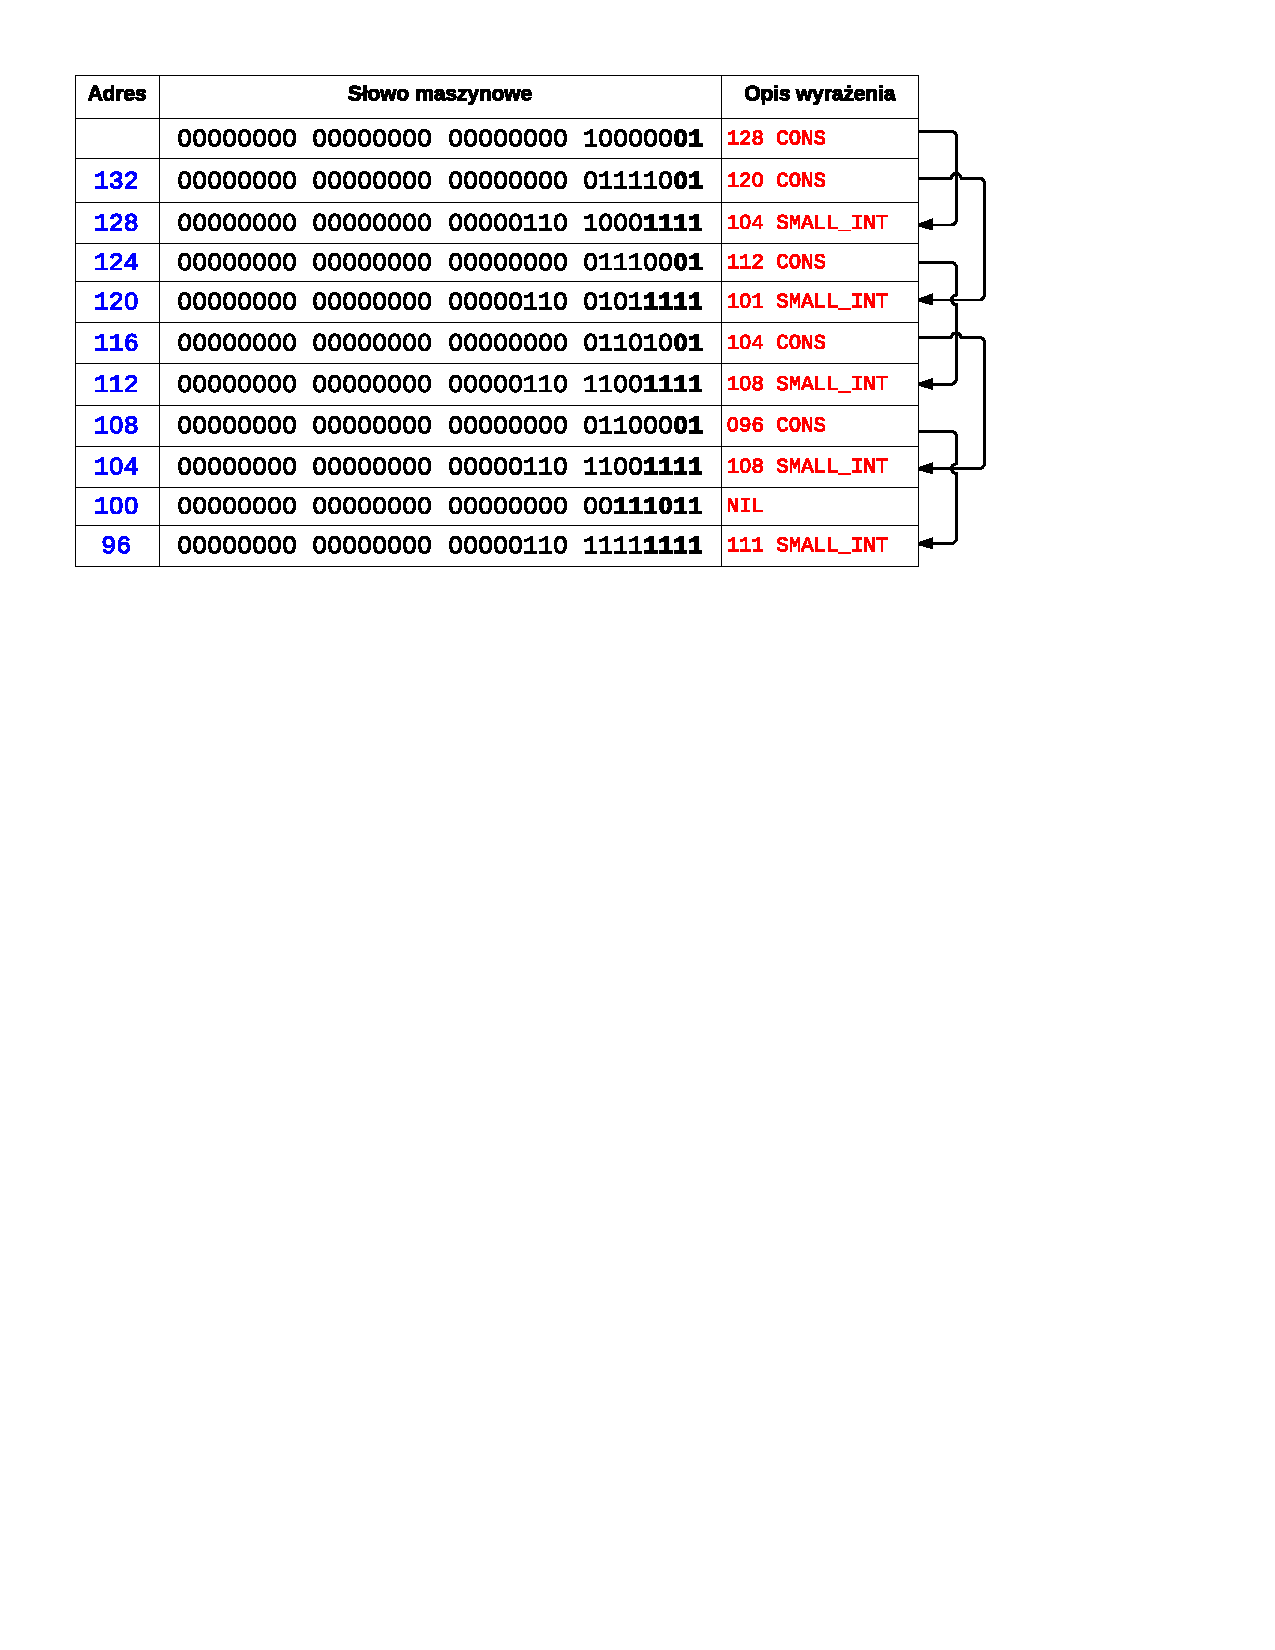
\includegraphics[scale=1, clip, trim=10mm 180mm 45mm 10mm]{list_on_heap}}
\caption{Przykład przechowywania listy na stercie procesu}
\label{fig:listonheap}
\end{figure}

Powyższy przykład dobrze ilustruje narzut pamięciowy jaki wprowadza sposób zapisu napisu przy użyciu listy. 
Informacja, która przy użyciu innych języków programowania może być zapisana przy użyciu 5 bajtów w języku Erlang potrzebuje aż 10 słów maszynowych (40 bajtów na architekturze 32-bitowej).
Receptą na tego typu problem, wprowadzoną w maszynie wirtualnej BEAM, jest binarny typ danych. Napis \texttt{"hello"} przy jego użyciu zajmowałby w pamięci 3 słowa maszynowe (nagłówek i~2~słowa przeznaczone na dane).
Typ ten jednak nie został zaimplementowany w obecnej wersji maszyny na system FreeRTOS.  

Jak można zauważyć zarówno złożoność obliczeniowa (czas dostępu do danych na liście jest liniowy) jak i pamięciowa przy wykorzystaniu tego typu danych jest dość znacząca.

\subsection{Krotki}
\label{sub:typyKrotki}

Kolejnym złożonym typem danym, z którego można korzystać w języku Erlang jest krotka, zajmująca spójny obszar pamięci. Z implementacyjnego punktu widzenia można porównać ją do tablicy zawierającej wyrażenia erlangowe.

Krotka jest jednym z typów opakowanych (\textbf{BOXED}), zatem referencja do niej z poziomu stosu procesu zawiera wskaźnik do nagłówka krotki. Nagłówek, podobnie jak pozostałe wyrażenia zajmuje jedno słowo maszynowe i przechowuje rozmiar krotki w postaci:
$$\texttt{AAAAAAAA AAAAAAAA AAAAAAAA AA\textbf{000000}}$$
gdzie bity \texttt{A} oznaczają rozmiar (arność) krotki. Wyrażenia wchodzące w skład krotki zajmują kolejne, następujące po nagłówku, słowa maszynowe.

Na rysunku \ref{fig:tupleonheap} zaprezentowany został przykład przechowywania danych wewnątrz krotki na stercie procesu, jak w przykładzie na rys. \ref{fig:listonheap}, czyli krotki \texttt{\{104,101,108,108,111\}}.

\begin{figure}[h]
\centerline{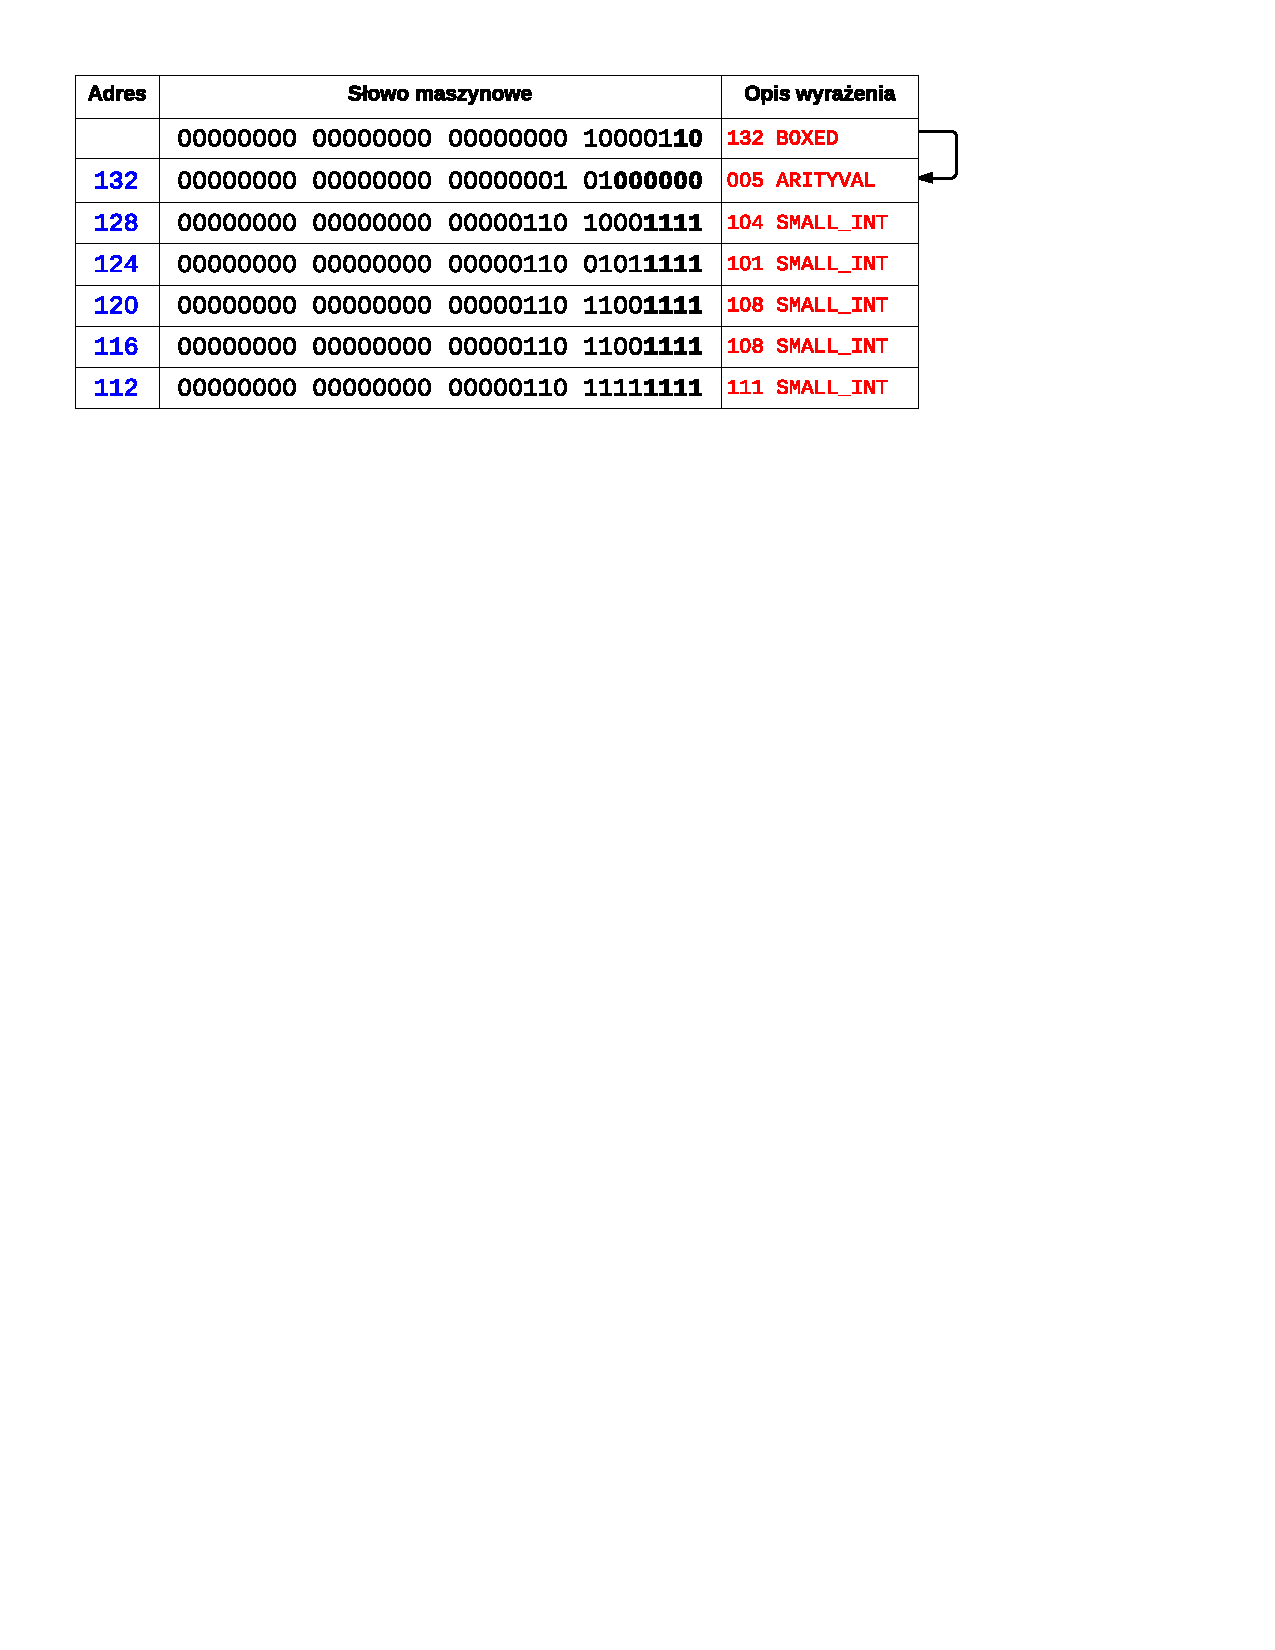
\includegraphics[scale=1, clip, trim=10mm 210mm 45mm 10mm]{tuple_on_heap}}
\caption{Przykład przechowywania krotki na stercie procesu}
\label{fig:tupleonheap}
\end{figure}

Ze względu na to, że krotka przechowuje dane w spójnym obszarze pamięci i dostęp do nich odbywa się w czasie stałym, użycie tego typu danych jest dobrym pomysłem w przypadku przechowywania danych tablicowych.

\subsection{Duże liczby}
\label{sub:typyBigs}

Drugim zaimplementowanym, opakowanym typem danych są duże liczby całkowite.
Wszystkie liczby całkowite, które nie mieszczą się w zakresie typu \textbf{SMALL\_INT}, czyli potrzebują do ich zapisania przynajmniej 29 bitów zapisywane są w typie danych \textbf{BIGNUM}.
Maszyna wirtualna zaimplementowana w ramach pracy, podobnie jak maszyna BEAM, implementuje własną arytmetykę implementującą operacje na tego typu liczbach.

Nagłówek typu \textbf{BOXED} ma w tym przypadku postać:
$$\texttt{AAAAAAAA AAAAAAAA AAAAAAAA AA\textbf{001S00}}$$
gdzie bity \texttt{A} oznaczają liczbę słów maszynowych, które składają się na całą liczbę bez znaku. Słowa te, w~kolejności od najmniej do najbardziej znaczącego, zajmują w pamięci kolejne słowa maszynowe po nagłówku. Bit \texttt{S} przechowuje znak liczby: \texttt{1} dla liczb ujemnych, {0} dla dodatnich.

Na rysunku \ref{fig:bignumonheap} zaprezentowany został przykład przechowania liczby $10^{28}$ na stercie procesu.

\begin{figure}[h]
\centerline{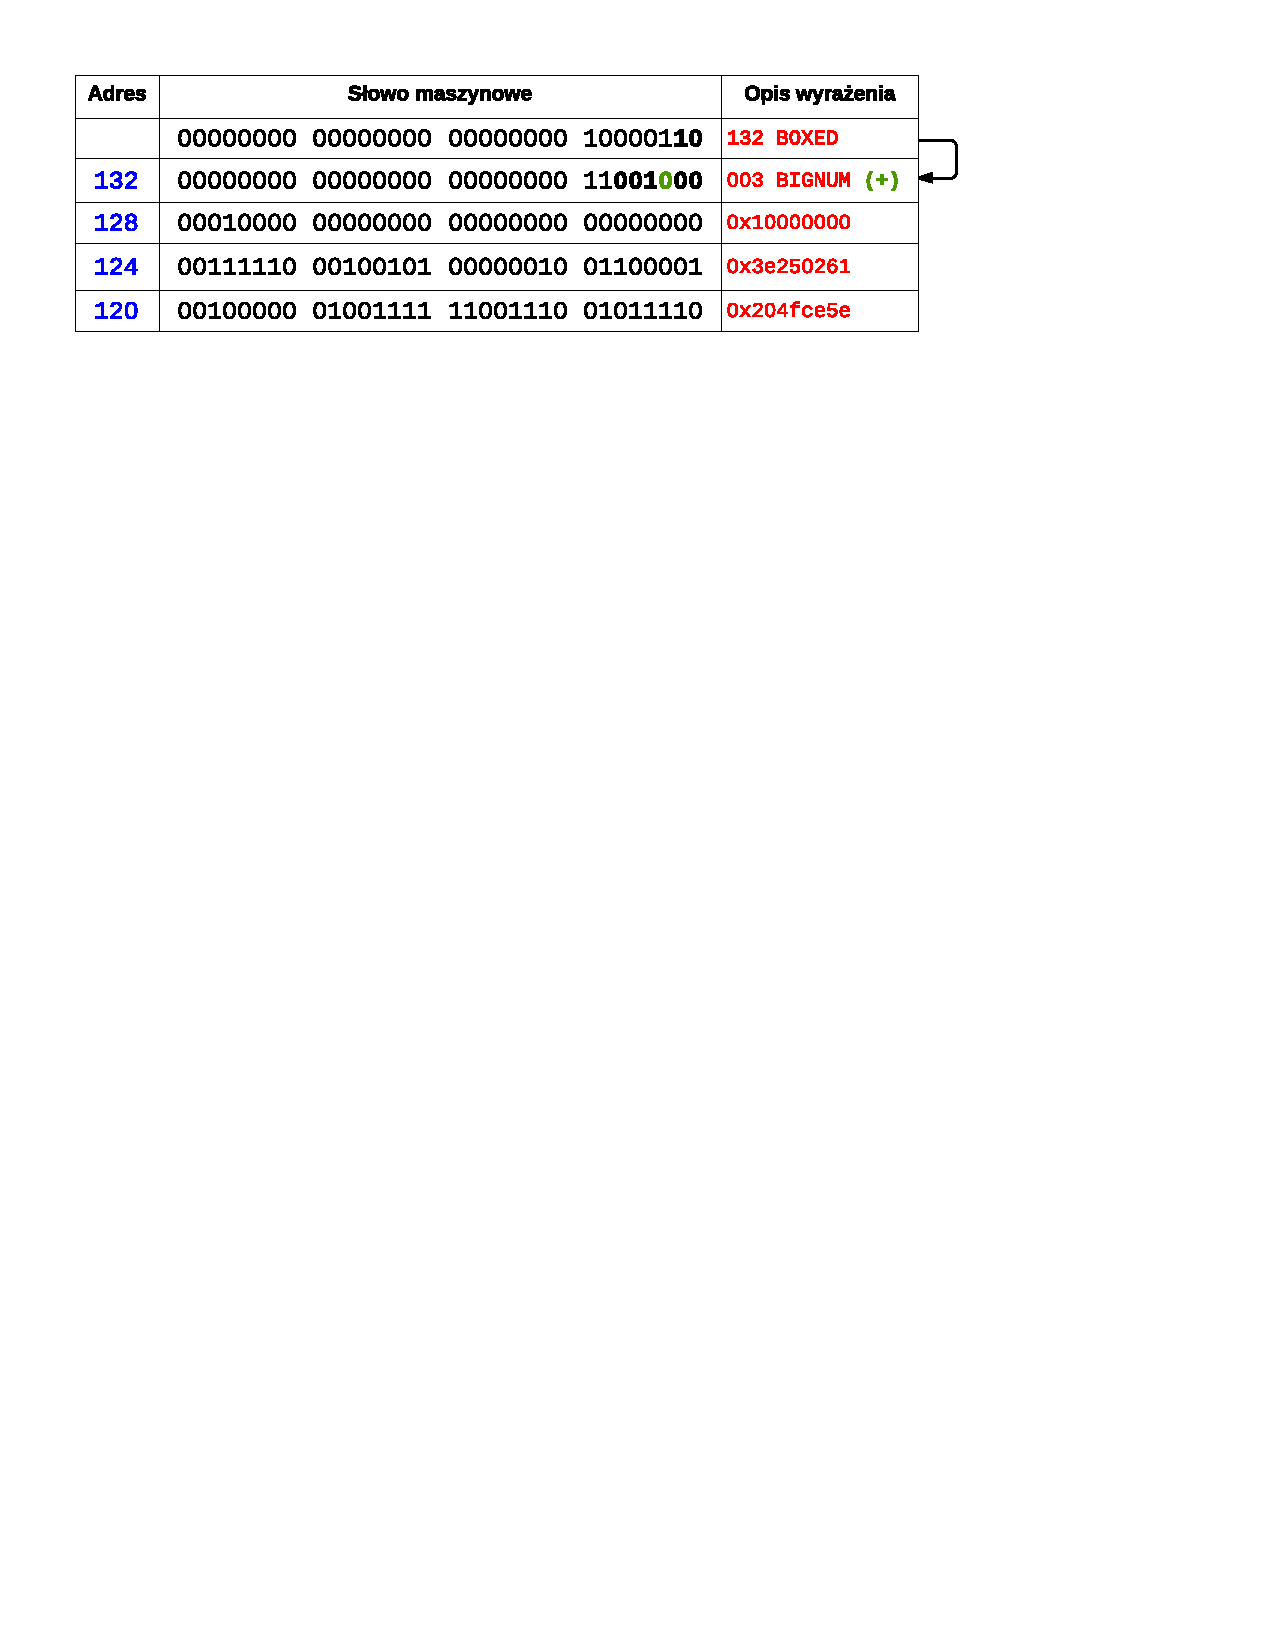
\includegraphics[scale=1, clip, trim=10mm 223mm 45mm 10mm]{bignum_on_heap}}
\caption{Przykład przechowywania dużej liczby na stercie procesu}
\label{fig:bignumonheap}
\end{figure}

\subsection{Lambdy}
\label{sub:typyLambda}

Typ danych wykorzystywany jest do identyfikacji obiektów funkcyjnych tworzonych dynamicznie w trakcie działania programu.
W maszynie wirtualnej BEAM obiekt taki może powstać w dwojaki sposób: przez wywołanie instrukcji \texttt{make\_fun2} lub funkcji wbudowanej \texttt{erlang:make\_fun/3}.
Bajty następujące po nagłówku typu danych zawierają informacje dotyczące miejsca początku kodu lambdy (każdemu obiektowi funkcyjnemu zdefiniowanemu w ramach danego modułu odpowiada osobna funkcja lokalna) a także wolnych zmiennych przez nią wykorzystywanych (czyli zmiennych, którym wartość przypisana została poza treścią lambdy, ale znajdujących się w jej kontekście).

Ten typ danych został w niniejszej maszynie wirtualnej zaimplementowany w ograniczonym zakresie, pozwalającym na definicję i wywołanie obiektów funkcyjnych w podstawowym zakresie.
Możliwe jest utworzenie lambdy poprzez jej zdefiniowanie, pod warunkiem że liczba jej wolnych zmiennych jest równa 0, lub na podstawie funkcji lokalnej (za pomocą konstrukcji \texttt{fun foo/2}).
Dodatkowo, utworzone lambdy nie podlegają odśmiecaniu przez algorytm \emph{garbage collectora}, dlatego też ich dynamiczne tworzenie w trakcie działania programu będzie prowadzić do wycieków pamięci.

Nagłówek typu danych ma następującą postać:
$$\texttt{00000000 00000000 00000000 00\textbf{000101}}$$

\subsection{Niezaimplementowane typy danych}
\label{sub:typyNiezaimplementowane}

Typy danych dostępne w maszynie BEAM, które nie zostały zaimplementowane w pracy to:
\begin{itemize}
\item \textbf{referencje} (tag \textbf{REF}) - referencje z~założenia używane są do oznaczania wiadomości wysyłanych do innych węzłów z uruchomioną maszyną wirtualną a klastrowanie nie jest wspierane przez implementowaną maszynę wirtualną;
\item \textbf{porty} (tag \textbf{PORT}) - porty używane są do identyfikacji procesów uruchomionych w systemie operacyjnym poza maszyną wirtualną Erlanga, a do których delegowane są pewne operacje, wykonywane na poziomie systemu operacyjnego. Wykonanie tych operacji (jak np. operacje na plikach) z~założenia może zająć pewien dłuższy okres czasu, co mogłoby zakłócić harmonogramowanie procesów. Typ danych nie został zaimplementowany, gdyż w maszynie wirtualnej wszystkie operacje wykonywane na poziomie mikrojądra zostały zaimplementowane przy pomocy funkcji wbudowanych (por. \ref{sec:maszynaBIF});
\item \textbf{liczby zmiennoprzecinkowe} (tag \textbf{FLONUM}) - ten typ danych również nie został zaimplementowany w~wersji maszyny opisywanej w pracy. Liczby zmiennoprzecinkowe rzadko wykorzystywane są w programowaniu urządzeń wbudowanych ze względu na bardzo duży narzut czasowych w przypadku mikrokontrolerów nie mających koprocesora (np. procesor ARM Cortex-M3 nie posiada FPU). M.in. z tego powodu do maszyny BEAM arytmetyka zmiennoprzecinkowa została dodana dopiero w wersji R8;
\item \textbf{binaria} (tagi \textbf{*\_BINARY}) - binarny typ danych włącznie ze wszystkimi operacjami dotyczącymi dopasowywania do nich zmiennych również nie został zaimplementowany w maszynie. Jest to funkcjonalność warta rozważenia w przypadku dalszej pracy nad maszyną ze względu na binarny charakter szeregowych interfejsów wejścia-wyjścia obsługiwanych przez mikrokontrolery. Podstawowe operacje na binariach do maszyny BEAM zostały dodane w wersji R7, bardziej zaawansowane były sukcesywnie dodawane od wersji R10;
\item \textbf{etykiety bloku \texttt{catch}} (tag \textbf{CATCH}) - typ danych służy do zapamiętywania na stosie procesu miejsc w kodzie, w których pojawiają się bloki \texttt{try} oraz \texttt{catch}. W przypadku błędu w programie, przed zakończeniem działania procesu, stos jest przeszukiwany w poszukiwaniu obecności ww. bloków. Instrukcje dotyczące łapania błędów nie zostały zaimplementowane w niniejszej maszynie wirtualnej.
\end{itemize}

%---------------------------------------------------------------------------
\section{Interpreter kodu maszynowego}
\label{sec:maszynaInterpreter}

Moduł opisany w niniejszym podrozdziale został zaimplementowany w pliku źródłowym \texttt{beam\_emu.c}.

\subsection{Maszyna stosowa a rejestrowa}
\label{sub:interpreterStosowa}

Spośród sposobów implementacji maszyny wirtualnej można wymienić dwa: maszynę stosową i~rejestrową.
Różnicę między tymi dwoma podejściami stanowi sposób przechowywania argumentów wywoływanej funkcji, miejsca zapisu wyniku jej wykonania oraz zmiennych tymczasowych przez nią używanych.

W przypadku maszyny stosowej dane te przechowywane są na stosie. Kolejne argumenty operacji umieszczane są na stosie za pomocą operacji \textbf{PUSH}, natomiast przed wykonaniem operacji zdejmowane są przez instrukcję \textbf{POP}. Instrukcje wykonywane przez maszynę wirtualną nie potrzebują zatem żadnych dodatkowych argumentów, gdyż te powinny być przed jej wywołaniem umieszczone na szczycie stosu, podobnie jak wynik zwrócony przez wykonaną instrukcję.

Z kolei w przypadku maszyny rejestrowej, powyższe informacje zapisywane są w zbiorze rejestrów.
Konsekwencją tego jest brak instrukcji manipulujących stosem w wykonywanym kodzie, co wpływa pozytywnie na szybkość działania interpretera kodu pośredniego.
Właściwe instrukcje wymagają jednak przekazania dodatkowych argumentów adresujących rejestry, w których znajdują się argumenty operacji i rejestr docelowy dla wyniku jej wykonania.
Efektem tego jest dłuższy zapis instrukcji w kodzie pośrednim niż w przypadku maszyny stosowej.
Dodatkowym atutem użycia rejestrów jest możliwość optymalizacji kodu polegającego na wyliczeniu i zapisaniu do rejestru pewnego pośredniego wyniku.
Wynik ten może następnie zostać wykorzystany przez kilka różnych instrukcji, zamiast wyliczania go od nowa przez każdą z nich.

Przykładami stosowych maszyn są maszyny języków takich jak Java czy .NET.
Z kolei przykładami maszyn rejestrowych są maszyny wirtualne języka Lua czy maszyna wirtualna Javy na system Android - Dalvik.

\subsection{Model interpretera}
\label{sub:interpreterModel}

Maszyna wirtualna języka Erlang (BEAM oraz maszyna zaimplementowana w pracy) jest również przykładem rejestrowej maszyny wirtualnej.

Interpreter korzysta z następujących rejestrów:
\begin{itemize}
\item rejestry \textbf{X\textsubscript{0}-X\textsubscript{255}} służące do przechowywania kolejnych argumentów z jakimi wywoływana jest funkcja, dodatkowo w rejestrze \textbf{X\textsubscript{0}} zapisywana jest wartość zwracana przez funkcję;
\item rejestry \textbf{Y} znajdujące się na stosie aktualnie uruchomionego procesu, służące do przechowywania zmiennych lokalnych;
\item rejestr \textbf{IP} przechowujący wskaźnik do aktualnie wykonywanej przez interpreter instrukcji;
\item rejestr \textbf{CP} przechowujacy adres powrotu - wskaźnik do instrukcji, którą interpreter powinien wykonać gdy nastąpi powrót z aktualnie wykonywanej funkcji.
\end{itemize}

Na listingu \ref{lis:maxS} zaprezentowany został przykładowy kod pośredni funkcji o arności 3, wyliczającej maksimum ze wszystkich jej argumentów, wykorzystujący do tego celu funkcję wbudowaną \texttt{erlang:max/2}. Wyjaśnienie działania poszczególnych operacji zostało zawarte w dodatku \ref{cha:operacjeBeam}.

\begin{lstlisting}[style=erlang, caption=Kod pośredni funkcji zwracającej maksimum z trzech argumentów, label=lis:maxS]
{allocate,1,3}.
{move,{x,2},{y,0}}.
{call_ext,2,{extfunc,erlang,max,2}}.
{move,{y,0},{x,1}}.
{call_ext_last,2,{extfunc,erlang,max,2},1}.
\end{lstlisting}

Na rysunkach od \ref{fig:max1} do \ref{fig:max8} zaprezentowano zawartość rejestrów X (interpretera) i Y (stos procesu) po wykonaniu poszczególnych operacji kodu powyższego dla argumentów: \texttt{5,7,9}. Zapis \texttt{\{l,1\}} oznacza, że wskaźnik do instrukcji wskazuje na linię 1 z przykładu na listingu \ref{lis:maxS}, z kolei \texttt{erlang:max/2} oznacza, że wskaźnik do instrukcji wskazuje na początek tej funkcji wbudowanej. Przez zapis \texttt{CP} rozumiana jest wartość wskaźnika \textbf{CP} w chwili wywołania funkcji. 

Jak można zauważyć na rys. \ref{fig:max1} wszystkie trzy argumenty zostały umieszczone w rejestrach \textbf{X}: 0,~1~i~2. Instrukcja \texttt{\{allocate,1,3\}}, znajdująca się w pierwszej linii powoduje rozszerzenie stosu procesu o 2 wyrażenia, z czego na szczycie stosu umieszczany jest adres powrotu, z jakim została wywołana funkcja, zapisany pod wskaźnikiem \textbf{CP}. Jeżeli w trakcie wykonania tej instrukcji konieczne byłoby uruchomienie \emph{garbage collectora}, drugi argument informuje o tym, że aktualnie w użyciu są 3 rejestry \textbf{X} i nie jest możliwe zwolnienie obszarów pamięci do których one się odnoszą.

W linii 2 (rys. \ref{fig:max3}) dokonane zostaje przeniesienie wyrażenia z rejestru \textbf{X\textsubscript{2}} do rejestru \textbf{Y\textsubscript{0}}, który jest pierwszym wyrażeniem na stosie poniżej jego szczytu.
Należy zauważyć, że pomimo wykorzystania stosu do zapisu zmiennych lokalnych, które nie zostaną zmodyfikowane pomiędzy wywołaniami funkcji, do operacji na nim nie wykorzystuje się operacji stosowych.
Nie należy zatem wiązać wykorzystania stosu procesu z faktem, że maszyna wirtualna jest maszyną stosową.

Przed wywołaniem funkcji \texttt{erlang:max/2} w linii 3, jako adres powrotu zostaje zapisana kolejna instrukcja w module, znajdująca się w linii 4. Argumentami wywoływanej funkcji są wartości znajdujące się w rejestrach \textbf{X\textsubscript{0}} i \textbf{X\textsubscript{1}}. Wywołana funkcja w momencie powrotu przepisuje wskaźnik powrotu (\textbf{CP}) na kolejną instrukcję do wykonania (\textbf{IP}). Wartość zwrócona z funkcji znajduje się w rejestrze \textbf{X\textsubscript{0}}. 

W linii 5 (rys. \ref{fig:max6}) wartość przechowywana na stosie zostaje przepisana do rejestru \textbf{X\textsubscript{1}}.
Drugie wywołanie funkcji \texttt{erlang:max/2} jest wywołaniem ogonowo-rekurencyjnym.
Dlatego też przykładowa funkcja odpowiedzialna jest za przywrócenie wskaźnika \textbf{CP} ze stosu i zwolnienie go jeszcze przed wywołaniem funkcji zewnętrznej. 
Wartość zwrócona z trójargumentowej funkcji znajduje się w rejestrze \textbf{X\textsubscript{0}}, a kolejna wykonana instrukcja będzie następująca po instrukcji, która ją wywołała.

\begin{figure}
\begin{multicols}{2}

\vspace{-4mm}
\begin{Figure}
 \centering
 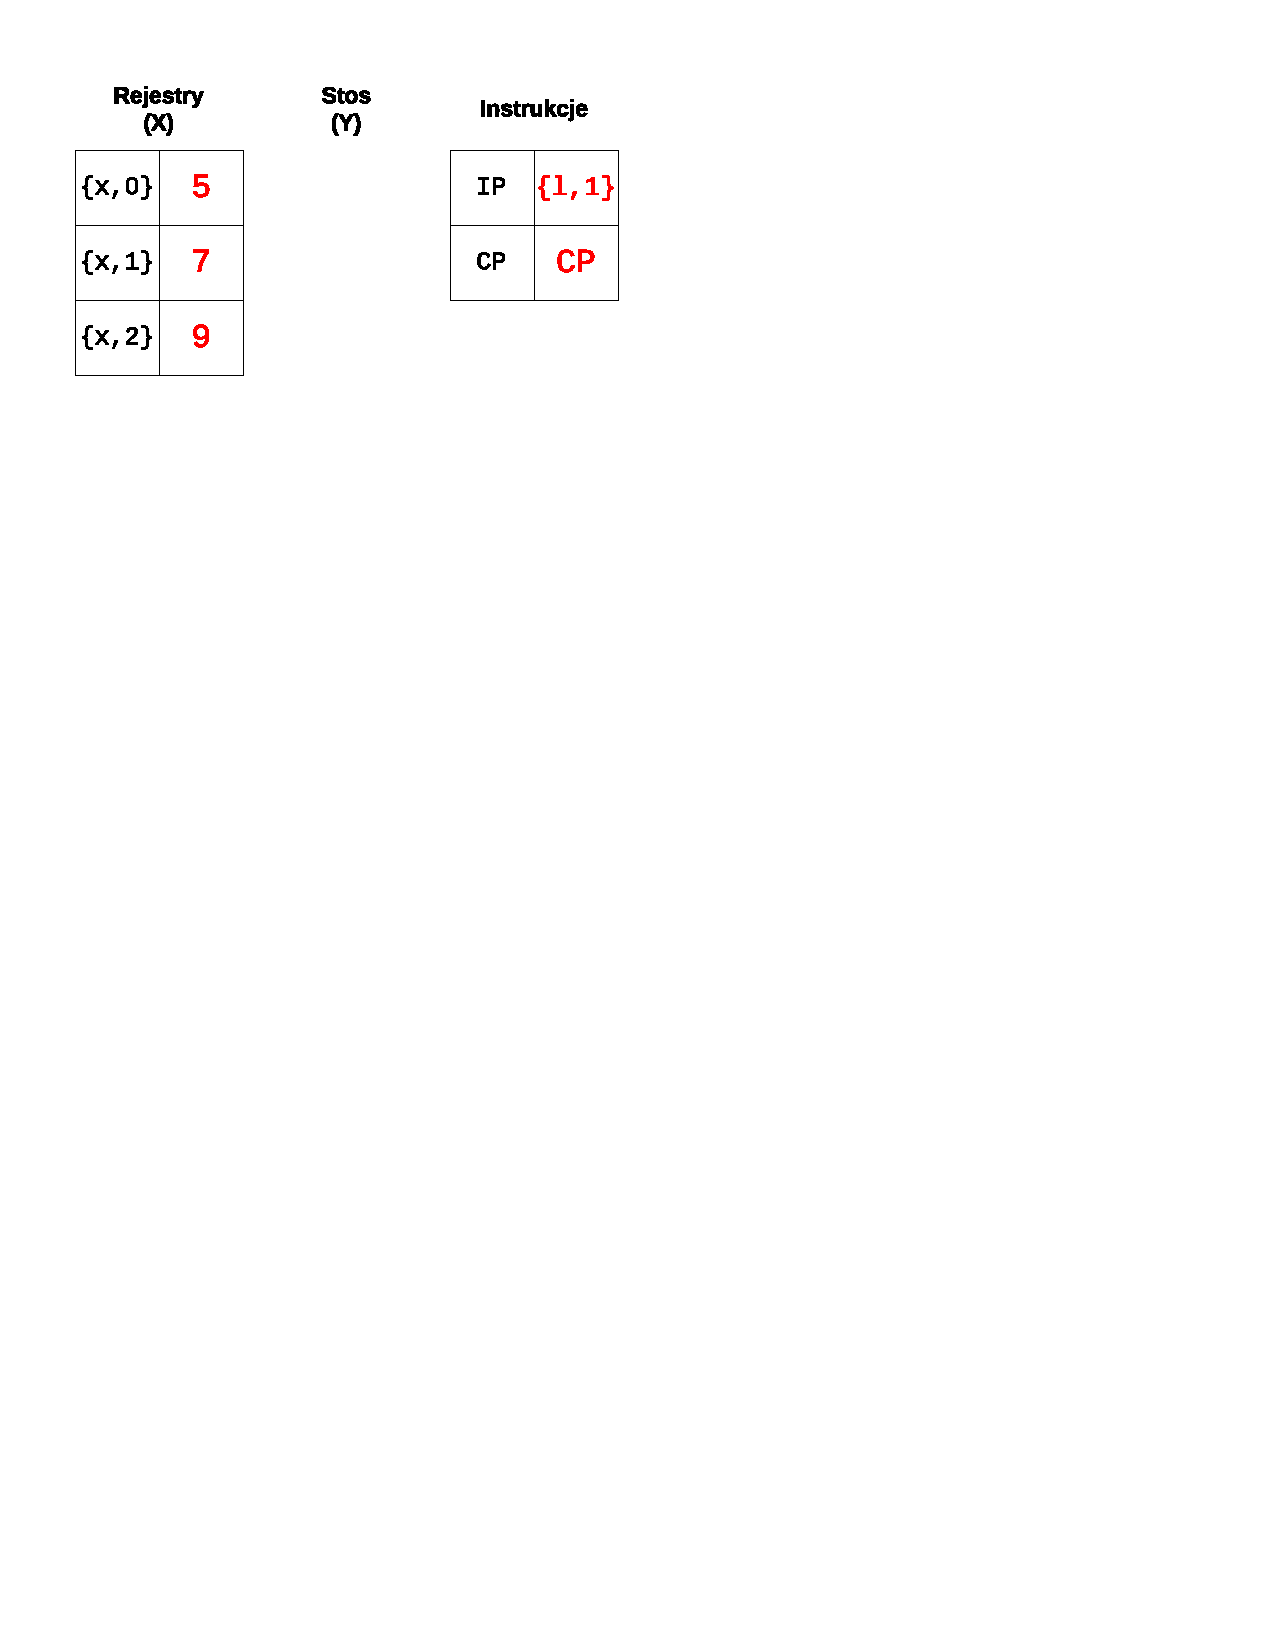
\includegraphics[scale=0.65, clip, trim=10mm 215mm 110mm 10mm]{interpreter_max_1}
\captionof{figure}{Rejestry przed wykonaniem instrukcji w linii 1}
\label{fig:max1}
\end{Figure}

\vspace{-4mm}
\begin{Figure}
 \centering
 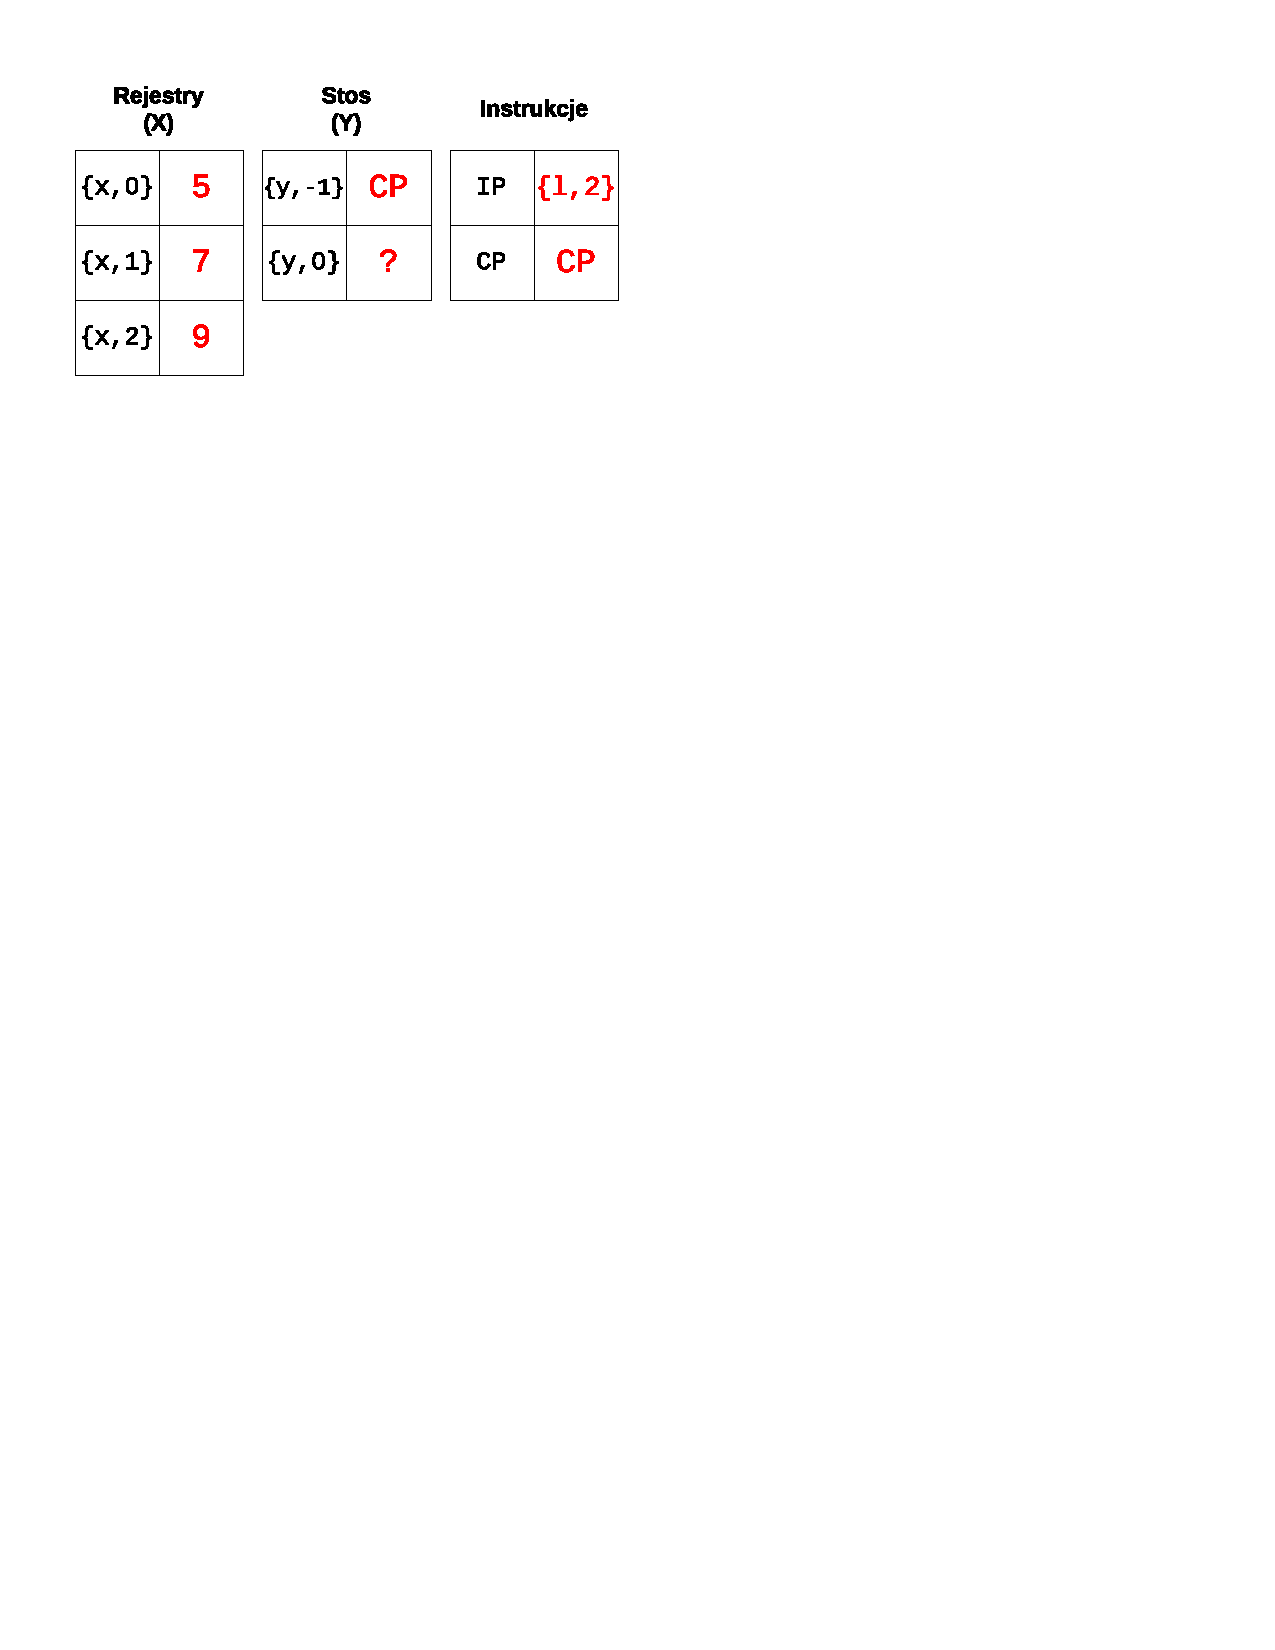
\includegraphics[scale=0.65, clip, trim=10mm 215mm 110mm 10mm]{interpreter_max_2}
\captionof{figure}{Rejestry przed wykonaniem instrukcji w linii 2}
\label{fig:max2}
\end{Figure}

\vspace{-4mm}
\begin{Figure}
 \centering
 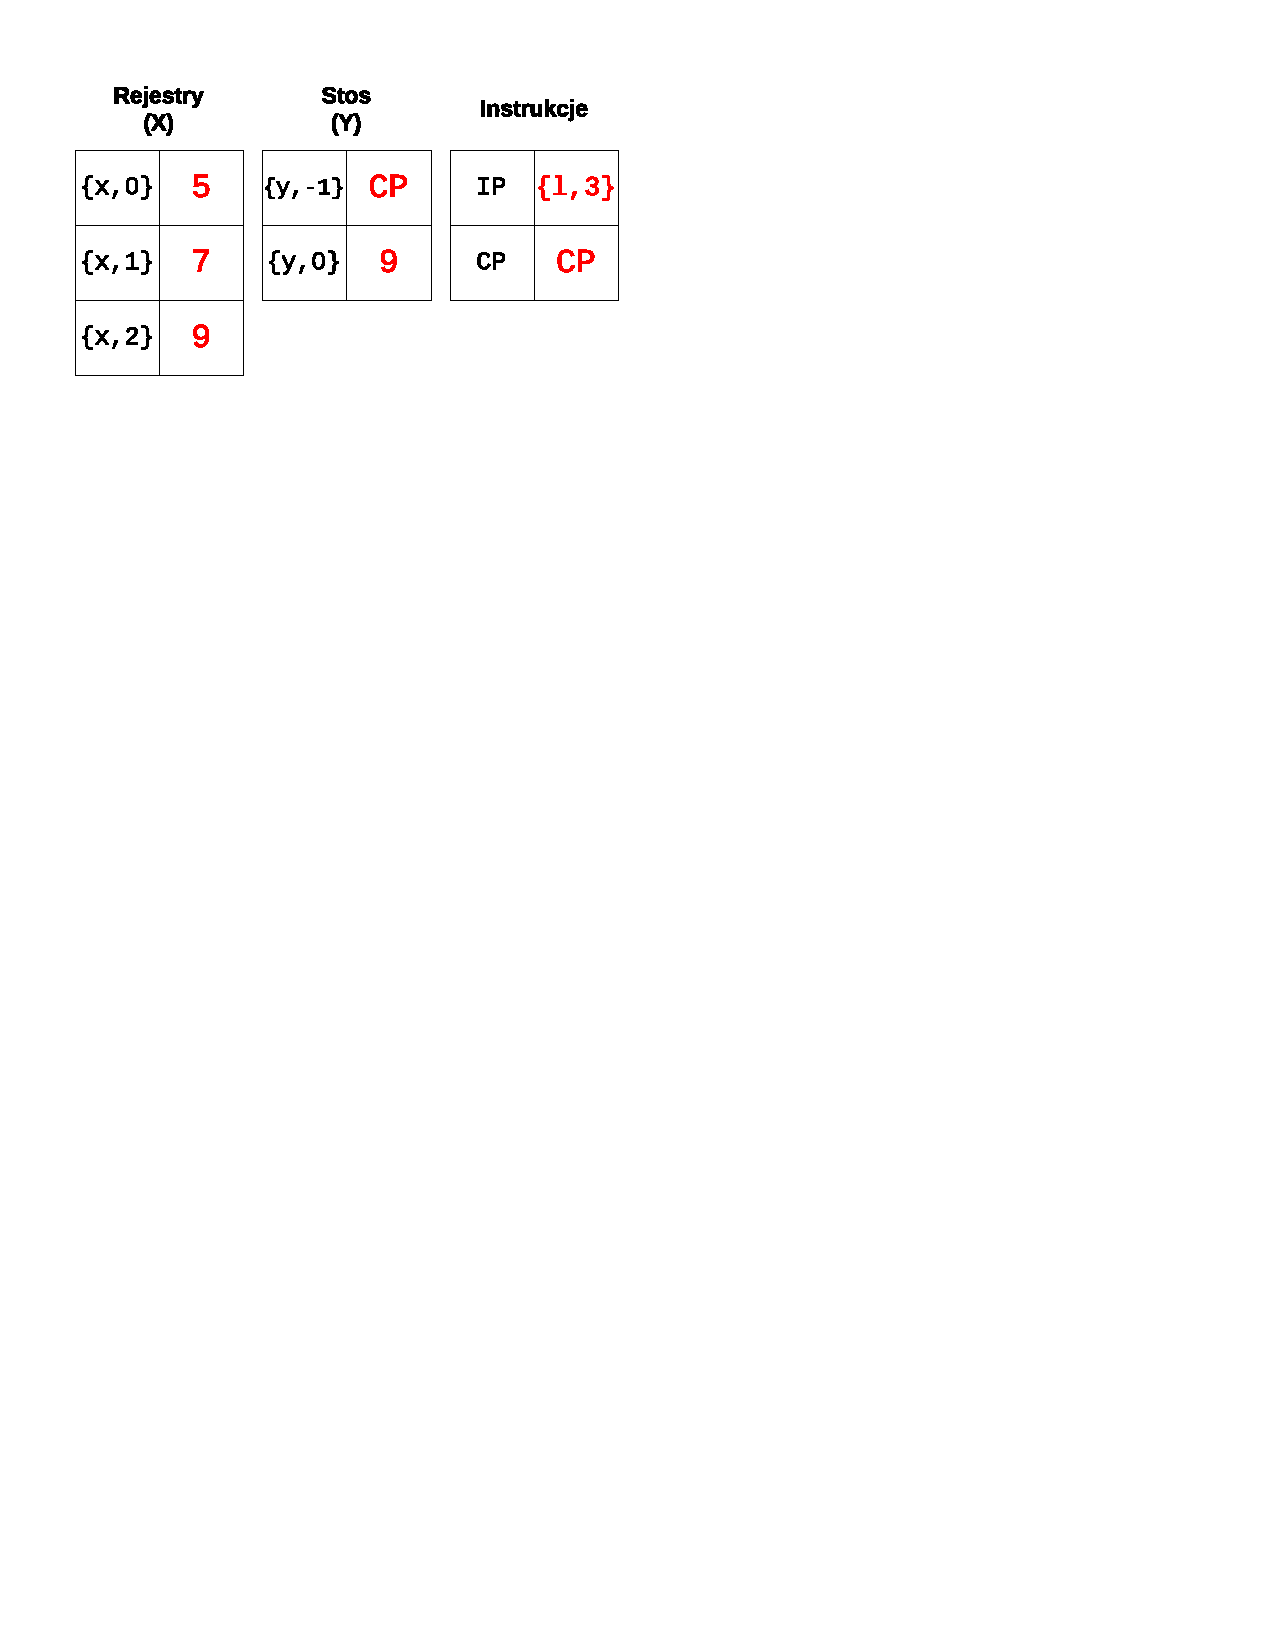
\includegraphics[scale=0.65, clip, trim=10mm 215mm 110mm 10mm]{interpreter_max_3}
\captionof{figure}{Rejestry przed wykonaniem instrukcji w linii 3}
\label{fig:max3}
\end{Figure}

\vspace{-4mm}
\begin{Figure}
 \centering
 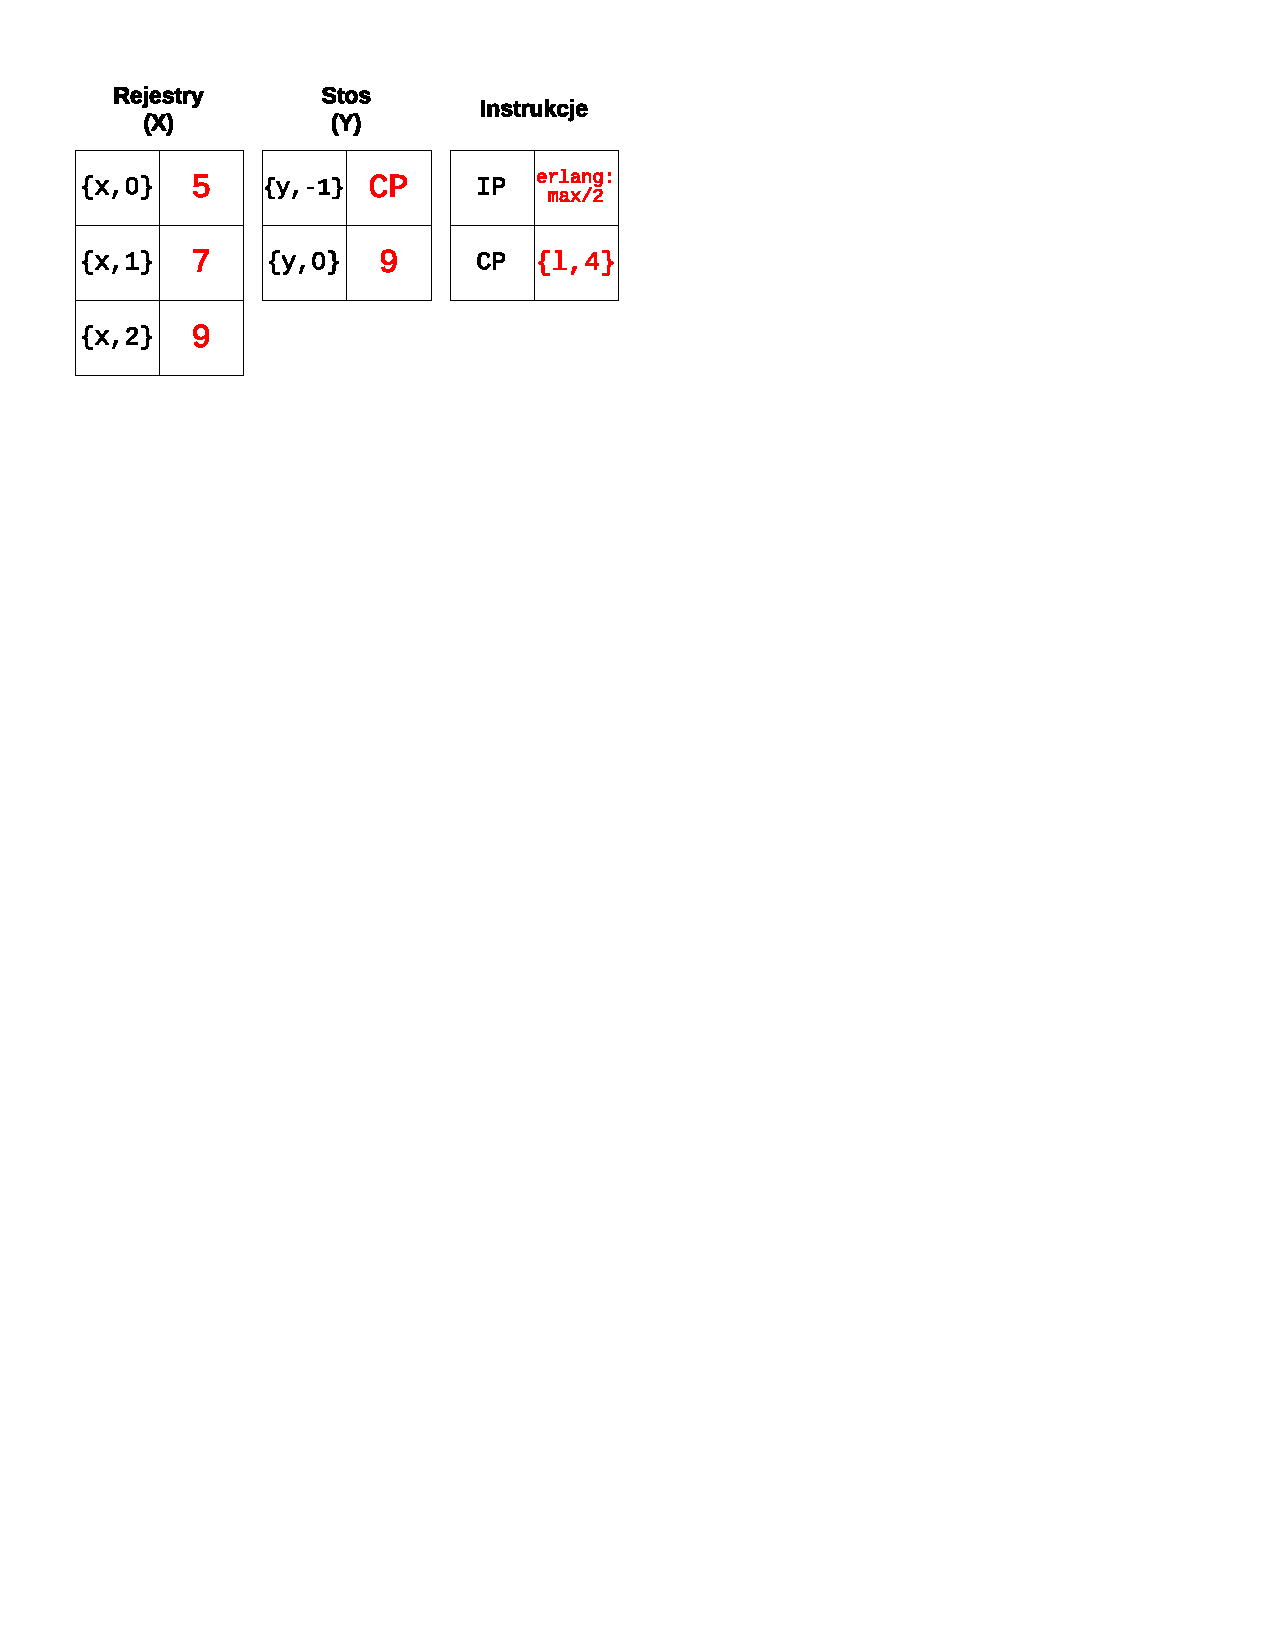
\includegraphics[scale=0.65, clip, trim=10mm 215mm 110mm 10mm]{interpreter_max_4}
\captionof{figure}{Rejestry przed wywołaniem funkcji w linii 3}
\label{fig:max4}
\end{Figure}

\vspace{-4mm}
\begin{Figure}
 \centering
 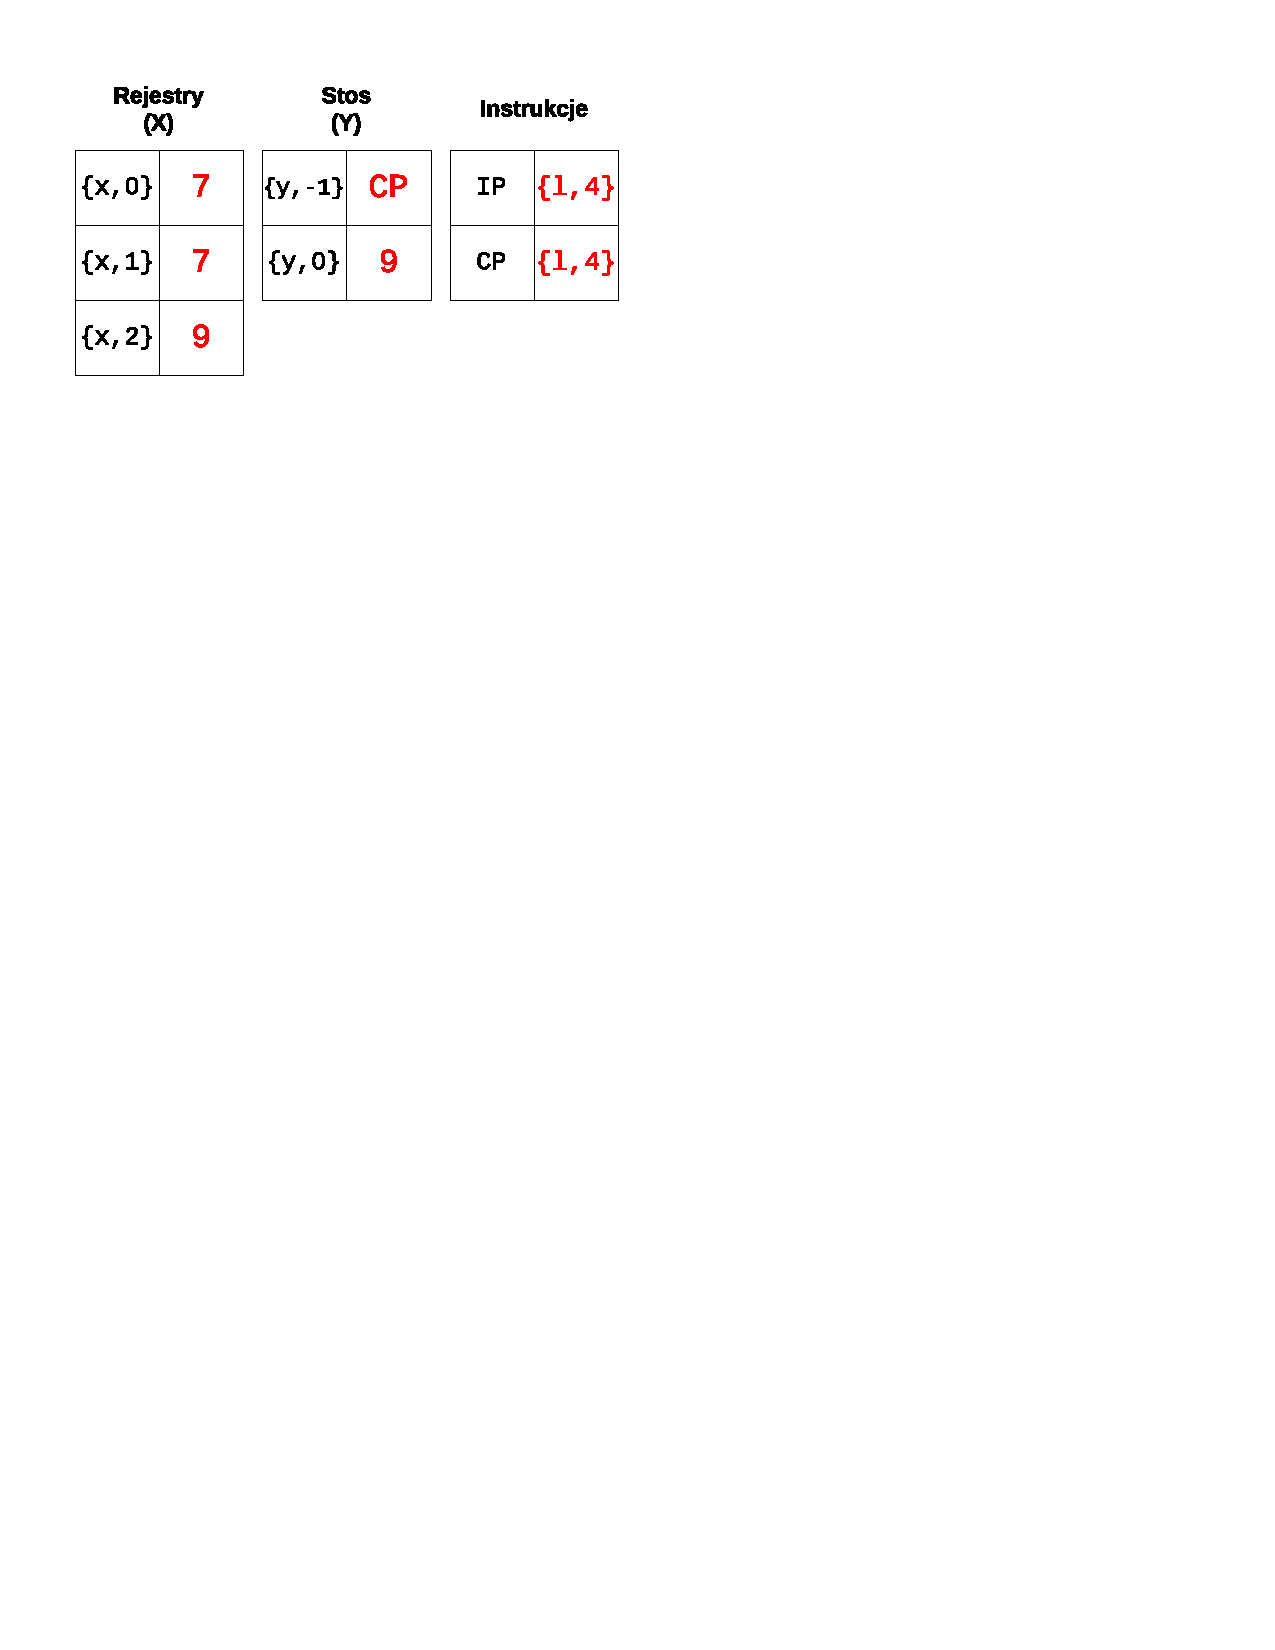
\includegraphics[scale=0.65, clip, trim=10mm 215mm 110mm 10mm]{interpreter_max_5}
\captionof{figure}{Rejestry przed wykonaniem instrukcji w linii 4}
\label{fig:max5}
\end{Figure}

\vspace{-4mm}
\begin{Figure}
 \centering
 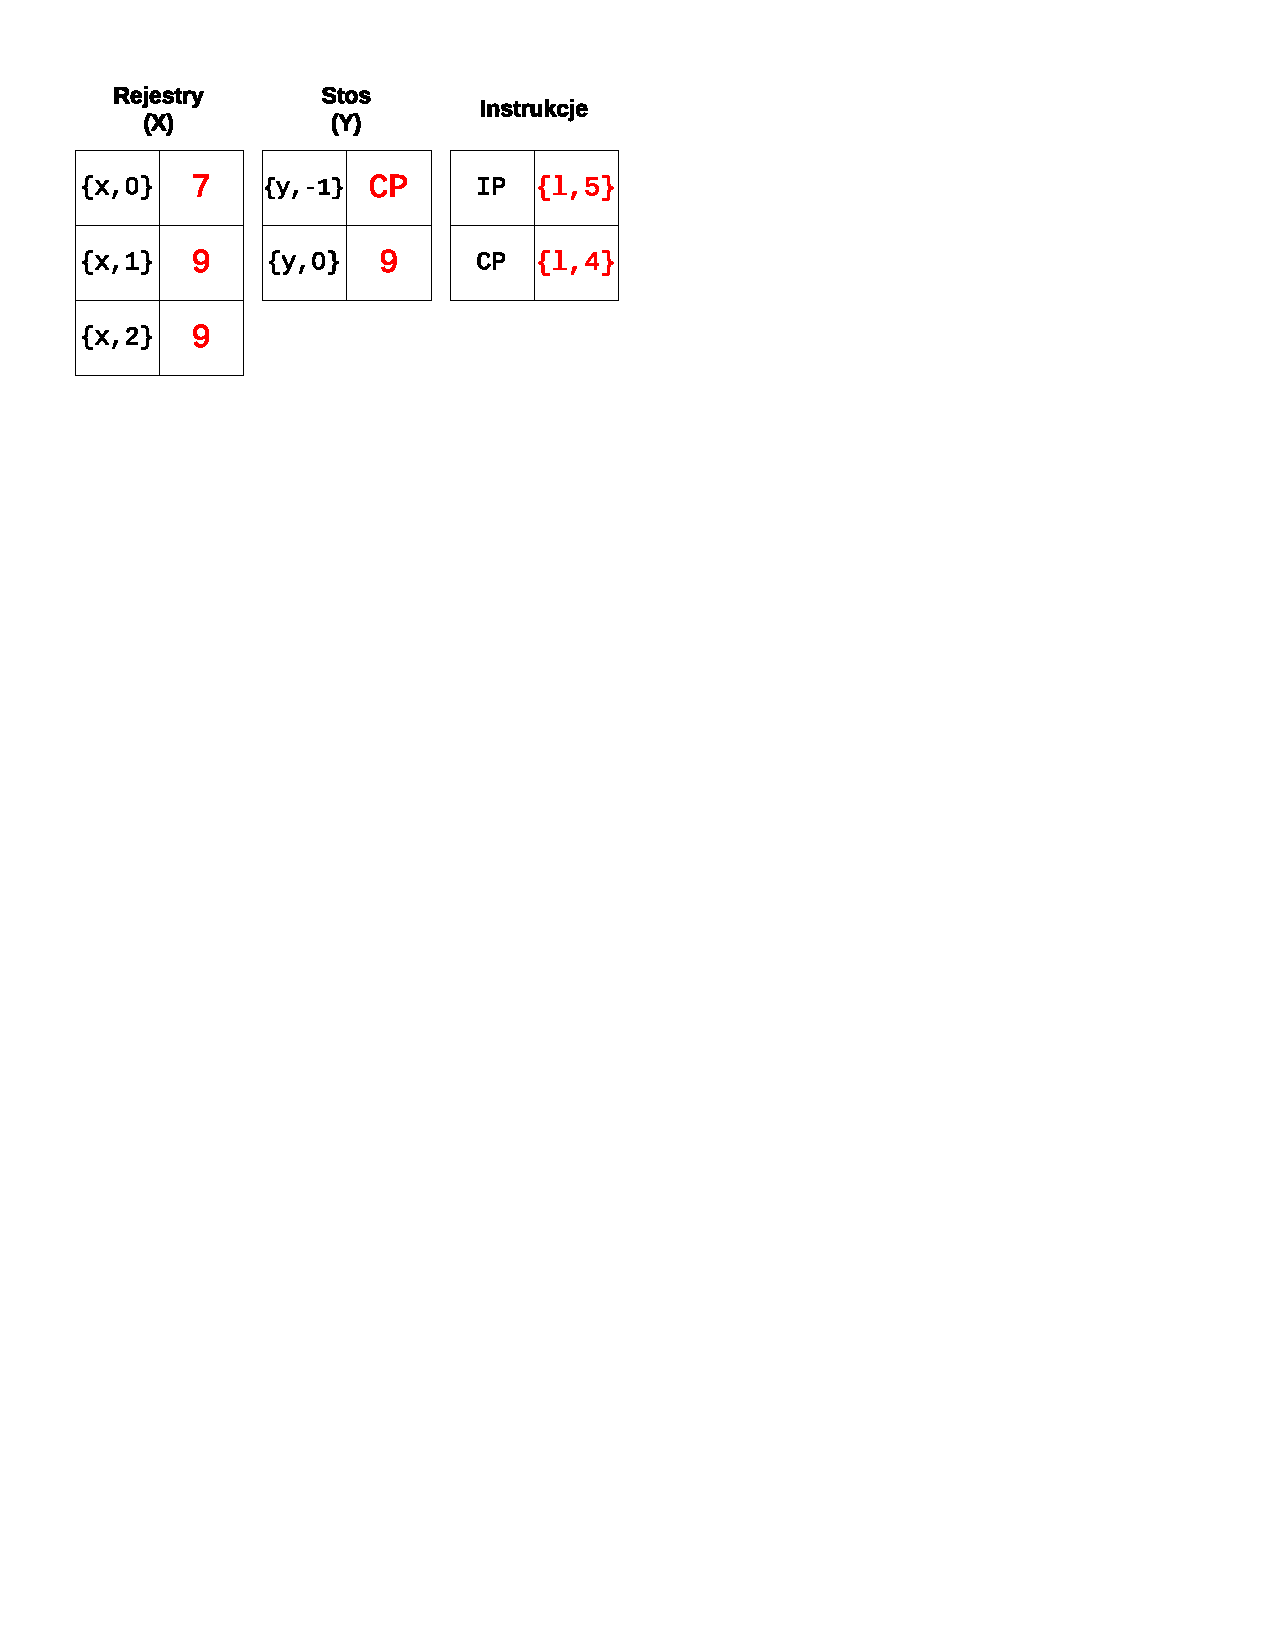
\includegraphics[scale=0.65, clip, trim=10mm 215mm 110mm 10mm]{interpreter_max_6}
\captionof{figure}{Rejestry przed wykonaniem instrukcji w linii 5}
\label{fig:max6}
\end{Figure}

\vspace{-4mm}
\begin{Figure}
 \centering
 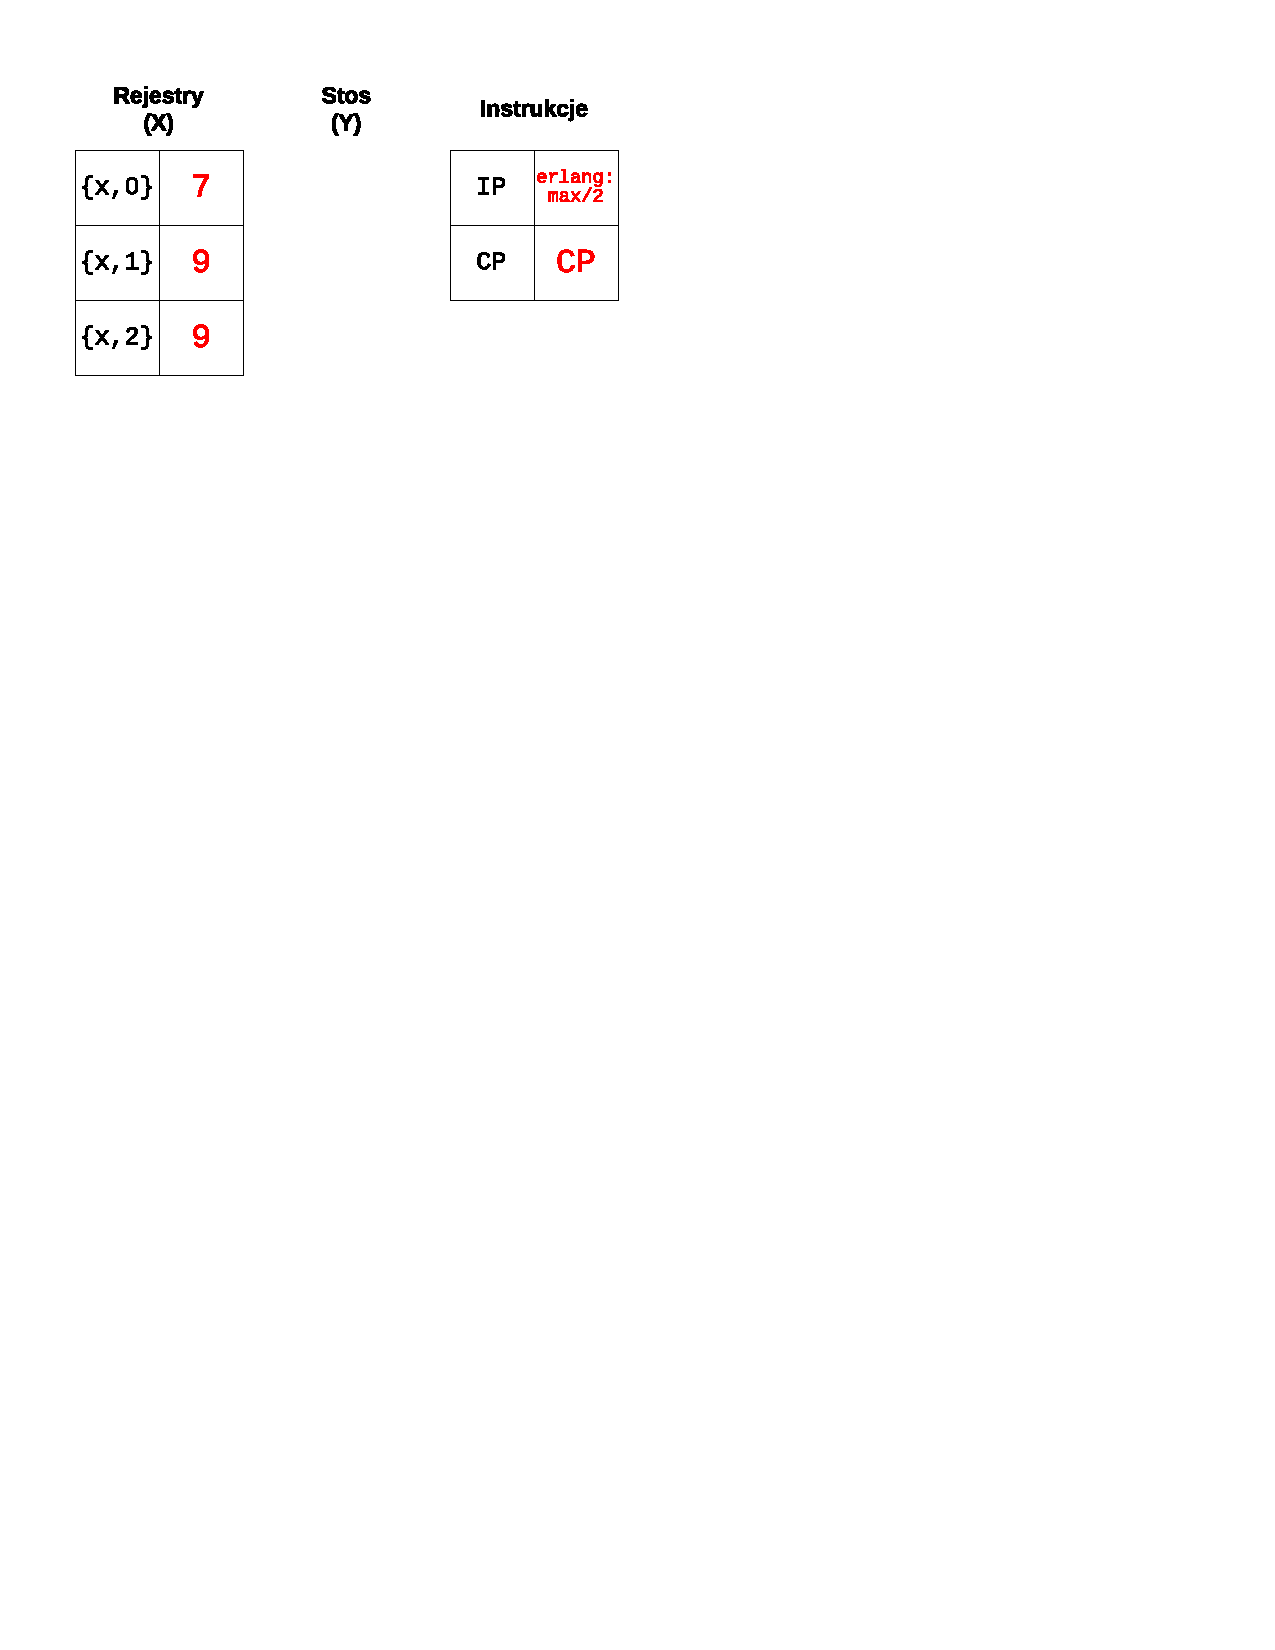
\includegraphics[scale=0.65, clip, trim=10mm 215mm 110mm 10mm]{interpreter_max_7}
\captionof{figure}{Rejestry przed wywołaniem funkcji w linii 5}
\label{fig:max7}
\end{Figure}

\vspace{-4mm}
\begin{Figure}
 \centering
 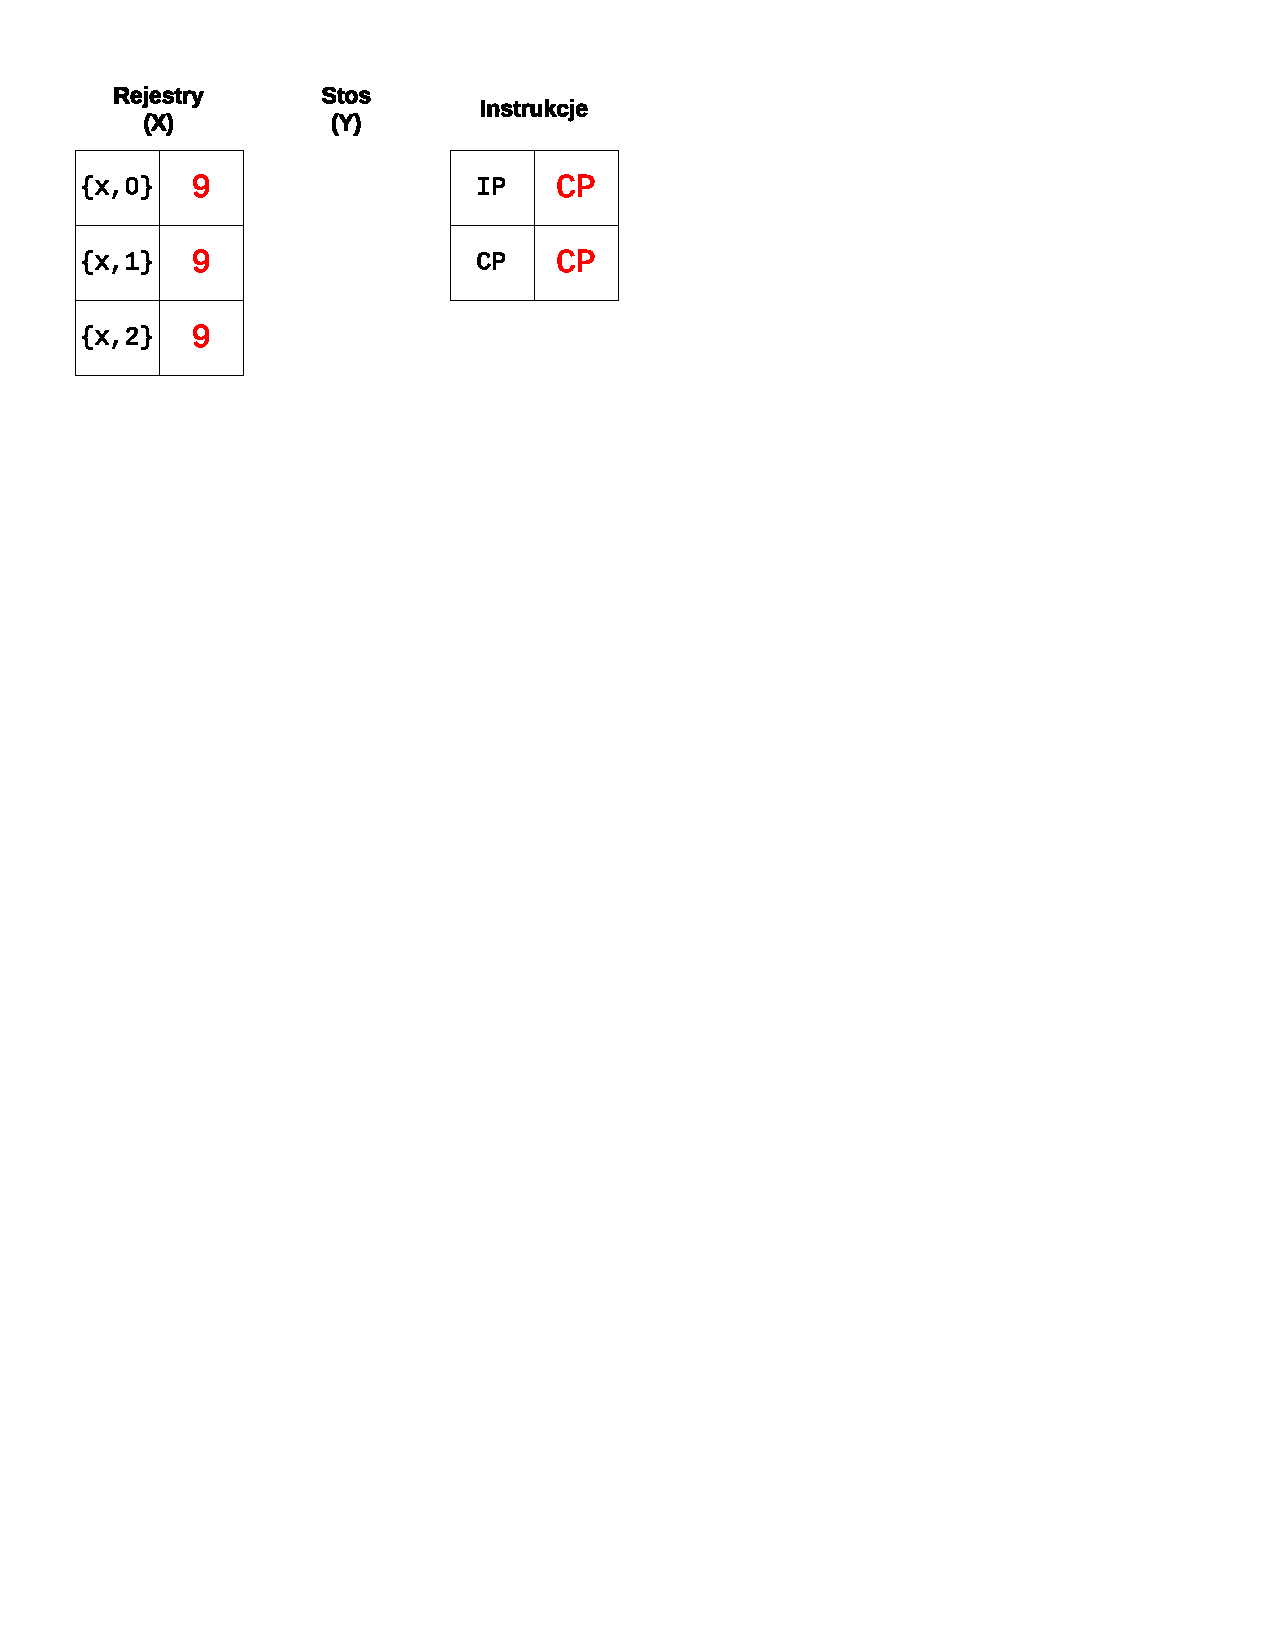
\includegraphics[scale=0.65, clip, trim=10mm 215mm 110mm 10mm]{interpreter_max_8}
\captionof{figure}{Rejestry po wykonaniu instrukcji w~linii 5, a zarazem i całej funkcji}
\label{fig:max8}
\end{Figure}
\end{multicols}
\end{figure}

\subsection{Sposób implementacji}
\label{sub:interpreterImplementacja}

Z implementacyjnego punktu widzenia kod interpretera kodu pośredniego w maszynie zaimplementowanej w pracy interpretuje kod adresowany bezpośrednio (\emph{Directly Threaded Code} \cite{Ertl}). Oznacza to, że operacja przekazywana do interpretera zapisana jest nie w postaci opkodu, ale zawiera wskaźnik do etykiety implementującej daną instrukcję. Odpowiedniej podmiany, w momencie ładowania pliku z modułem dokonuje \emph{loader}.

Maszyna wirtualna BEAM implementuje także sposób adresowania operacji przez ich opkod, na wypadek gdyby kompilator języka C użyty do jej kompilacji nie obsługiwał rozszerzenia standardu GNU C,~jakim są wskaźniki do etykiet.
Metoda \emph{Switch Threading} nie wymaga podmiany w żaden sposób oryginalnych opkodów, jednak interpretacja kodu pośredniego z jej użyciem jest dużo wolniejsza.
Powodem tego jest fakt, że kod każdej operacji przed jej wykonaniem należy sprawdzić z całym zestawem obsługiwanych opkodów w instrukcji \texttt{switch}, aż do napotkania właściwej.
W maszynie na system FreeRTOS wykorzystano oba sposoby adresowania operacji, a używany może zostać wybrany na poziomie konfiguracji maszyny wirtualnej (por. \ref{cha:config}).

Zestaw instrukcji zaimplementowanych w maszynie wirtualnej wraz z opisem ich działania został zaprezentowany w dodatku \ref{cha:operacjeBeam}.
Dodatek ten wymienia operacje, jakie możliwe są do otrzymania w pliku z kodem pośrednim z kompilatora języka Erlang.
Maszyna wirtualna BEAM implementuje jednak nieco większy zestaw instrukcji, który zostaje podmieniany w kodzie maszynowym w momencie ładowania modułu do pamięci (por. \ref{sec:maszynaLoader}).

Dodatkowymi operacjami, wykorzystywanymi wewnętrznie przez maszynę wirtualną, zaimplementowanymi w interpreterze są: \texttt{beam\_apply/0} oraz \texttt{normal\_exit/0}, służące do kontroli cyklu życia procesu.
W momencie startu procesu jako pierwsza instrukcja do wykonania (wskaźnik \textbf{IP}) zostaje ustawiona pierwsza z tych operacji, po wcześniejszym zapisaniu do pierwszych trzech rejestrów \textbf{X}: modułu, funkcji i listy argumentów będących początkowymi dla tego procesu.
Następnie operacja ta wywołuje właśnie tę funkcję.
Jako adres powrotu z wywołania funkcji początkowej (wskaźnik \textbf{CP}) ustawiana jest druga z dodatkowych instrukcji, która kończy działanie procesu z powodu osiągnięcia końca jego kodu.

%---------------------------------------------------------------------------
\section{Procesy}
\label{sec:maszynaProcesy}

Logika procesu opisana w niniejszym podrozdziale została zaimplementowana w pliku źródłowym \texttt{erl\_process.c}.

\subsection{Tablica procesów}
\label{sub:procTablica}

Stuktura procesów przechowywana jest w prealokowanej tablicy o konfigurowalnym rozmiarze.
W~zaimplementowanej maszynie domyślnie rozmiar ten wynosi 25.
Tak mała liczba procesów została wybrana ze względu na duże ograniczenia zasobów platformy docelowej dla maszyny.

Procesy identyfikowane są wewnątrz maszyny wirtualnej przez identyfikator procesu (\textbf{PID}, por. \ref{sub:typyImmediates}).
Ten bezpośredni typ danych przechowuje indeks procesu w ww. tablicy, dzięki czemu możliwe jest szybkie znalezienie struktury procesu, który konieczny jest do wykonania instrukcji przez interpreter kodu.

\subsection{Struktura procesu}
\label{sub:procStruktura}

W strukturze przechowującej informacje o procesie zostały zawarte dane niezbędne do poprawnego wykonywania przez niego kodu.
Spośród nich można wymienić:
\begin{itemize}
\item wspomniany wcześniej identyfikator procesu (\textbf{PID});
\item blok pamięci zajmowany przez wyrażenia wykorzystywane przez proces, zawierający stertę i stos. Został on szczegółowo opisany w podrozdziale \ref{sec:maszynaGC};
\item wskaźniki przechowujące aktualnie wykonywaną przez proces instrukcję oraz adres powrotu;
\item liczba redukcji jakie pozostały do wywłaszczenia procesu;
\item uchwyt do zadania w systemie FreeRTOS, w kontekście którego wykonywany jest kod procesu;
\item pamięć do przechowania wartości rejestrów \textbf{X} w sytuacji gdy proces przestanie być wykonywany na rzecz innego procesu (por. \ref{sec:maszynaScheduler});
\item kolejka wiadomości, które zostały wysłane do procesu;
\item lista procesów połączonych z danym procesem poprzez \emph{link} (por. \ref{sec:maszynaBledy});
\item flagi procesu, ustawiane przez funkcję \texttt{erlang:process\_flag/2};
\item informacje statystyczne związane z cyklem życia procesu, takie jak liczba wykonanych redukcji czy liczba wykonanych odśmieceń na procesie w trakcie jego działania.
\end{itemize}

Podstawową różnicą między implementacją maszyny a maszyny BEAM jest sposób wykonywania kodu pośredniego procesu.
Maszyna BEAM implementuje własny algorytm harmonogramowania, biorąc na siebie odpowiedzialność za utrzymywanie kolejki procesów do wykonania i zarządzania kolejnością ich wykonania. Logika procesu nie jest zatem opakowana w żadną warstwę abstrakcji. 
Z kolei maszyna zaimplementowana w pracy do zarządzania kolejnością procesów wykorzystuje \emph{scheduler} wbudowany w mikrojądro FreeRTOS, a procesy są instancjami zadań przez niego zarządzanych (por. podrozdział \ref{sec:rtosScheduler}).
Powodem wykorzystania takiego podejścia jest mały narzut pamięciowy i czasowy związany z uruchamianiem zadań, a także wbudowana obsługa priorytetów zadań i możliwość konfiguracji parametrów planisty.

Różnicą w strukturze procesu jest także uproszczenie obszaru pamięci dla wyrażeń procesu do jednej, podstawowej sterty. 
Maszyna BEAM wykorzystuje bardziej zaawansowane, generacyjne podejście przechowując wyrażenia na dwóch stertach.
Technika ta opisana została w podrozdziale \ref{sec:maszynaGC}.

W maszynie rozważanej w pracy nie została także zaimplementowany słownik procesu.

\subsection{Komunikacja międzyprocesowa}
\label{sub:procKolejka}

Komunikacja między procesami w maszynie wirtualnej jest zapewniona dzięki instrukcjom:
\begin{itemize}
\item \texttt{send}, służącej do wysłania wiadomości do innego procesu;
\item \texttt{wait} i \texttt{wait\_timeout} zawieszających działanie procesu aż do momentu otrzymania wiadomości lub przeterminowania;
\item \texttt{loop\_rec}, \texttt{remove\_message} i \texttt{loop\_rec\_end}, wykonujących operacje na kolejce wiadomości.
\end{itemize}

Mechanizm wysyłania wiadomości do procesu został zaprezentowany na rysunkach od \ref{fig:mp1} do \ref{fig:mp4}.

Na początku (rys. \ref{fig:mp1}) w kolejce wiadomości procesu odbierającego znajduje się jedna wiadomość (\textbf{M\textsubscript{0}}).
Wskaźnik aktualnej wiadomości ustawiony jest na pierwszą wiadomość w kolejce, oznaczoną kolorem czerwonym.
Zostanie on wykorzystany przez proces w momencie osiągnięcia przez kod procesu bloku \texttt{receive}.

\begin{figure}[h]
\centerline{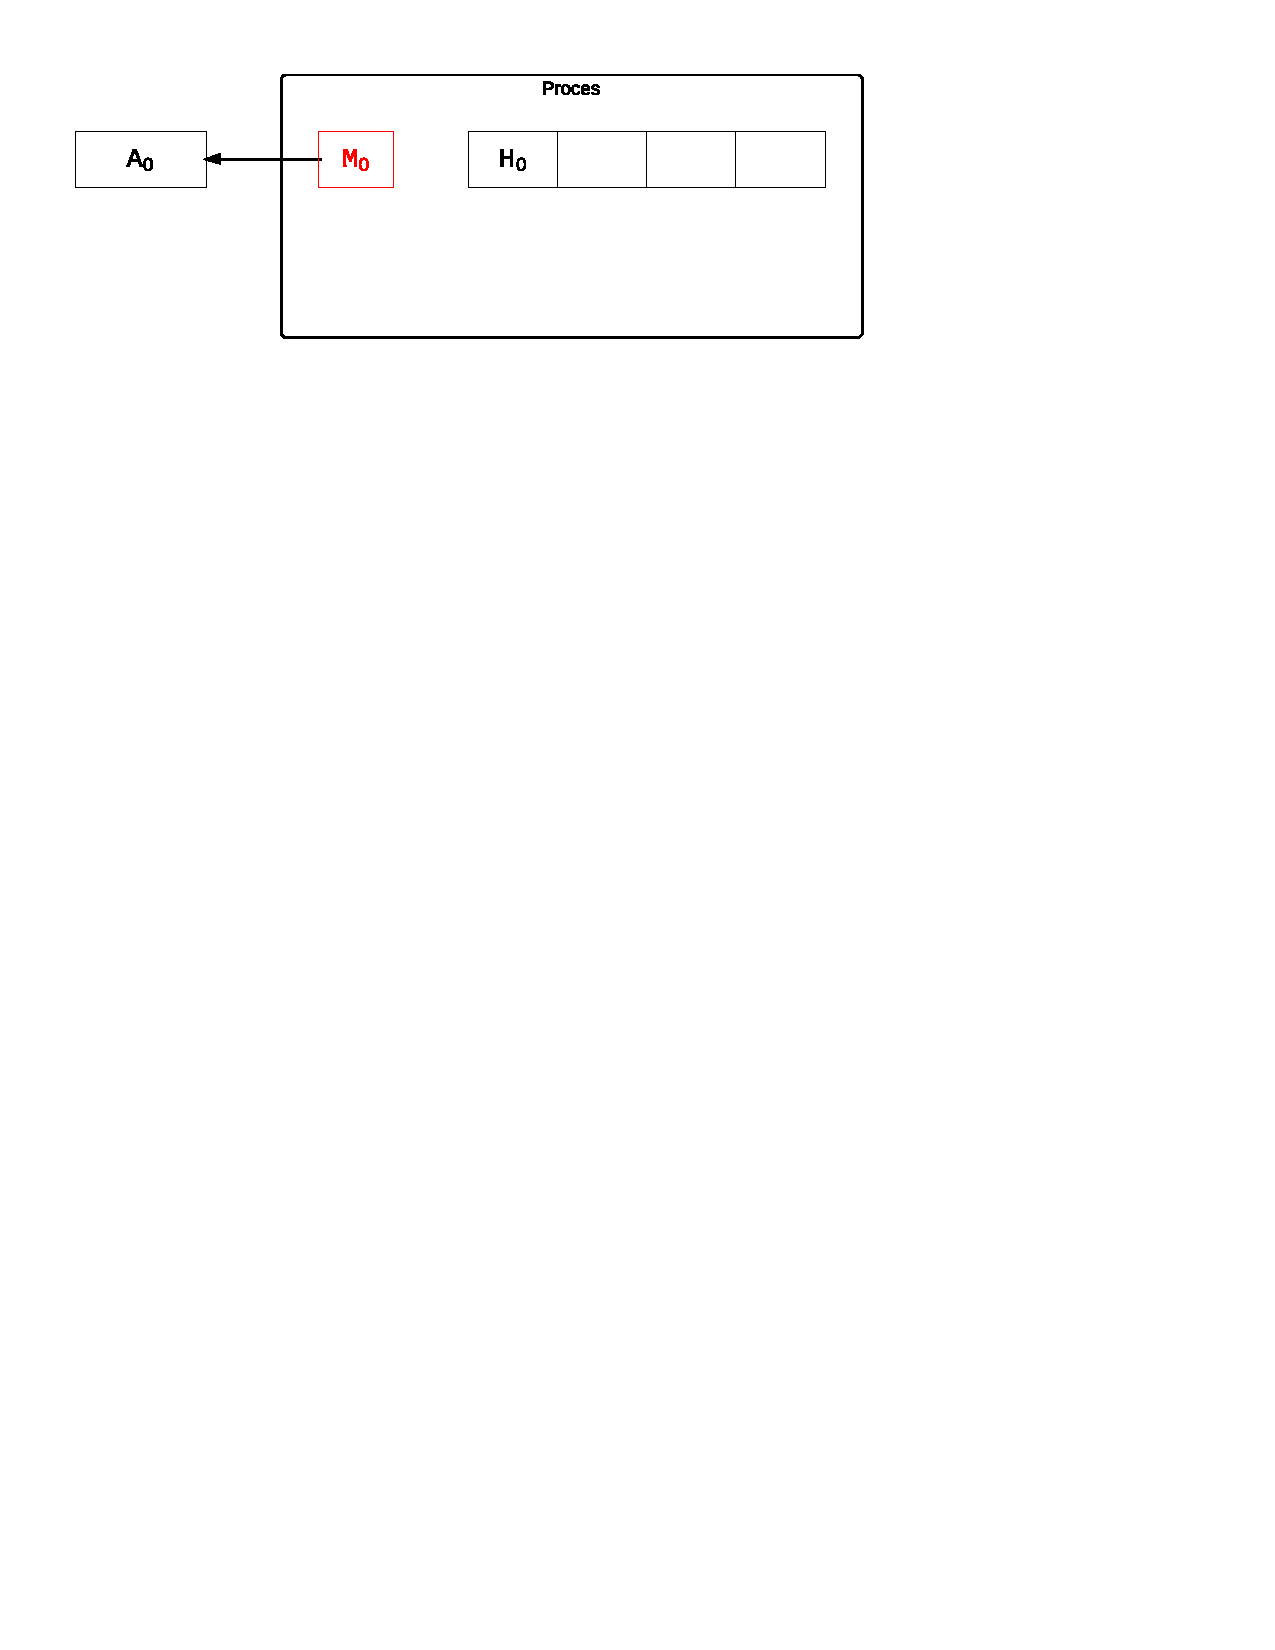
\includegraphics[scale=0.75, clip, trim=10mm 220mm 68mm 10mm]{mp1}}
\caption{Kolejka wiadomości procesu z jedną, nieodczytaną wiadomością.}
\label{fig:mp1}
\end{figure}

Wysłanie wiadomości do procesu polega na dołączeniu na koniec kolejki (która zaimplementowana jest jako lista jednokierunkowa) nowej wiadomości (rys. \ref{fig:mp2}).
Jeżeli wysyłane wyrażenie nie jest bezpośredniego typu danych, całe wyrażenie jest kopiowane do obszaru pamięci poza pamięcią należącą do procesu-odbiorcy.
Wiadomość nie jest kopiowana bezpośrednio na stertę procesu, gdyż w sytuacji w której na stercie nie byłoby wystarczającej ilości miejsca, konieczne byłoby uruchomienie \emph{garbage collectora}.
Tutaj pamięć zajmowana przez treść wiadomości została oznaczona przez \textbf{A\textsubscript{0}} oraz \textbf{A\textsubscript{1}}.
Jego uruchomienie powinno jednak zawsze mieć miejsce w bezpiecznym miejscu kodu, w którym znany jest cały źródłowy zbiór wyrażeń.


\begin{figure}[h]
\centerline{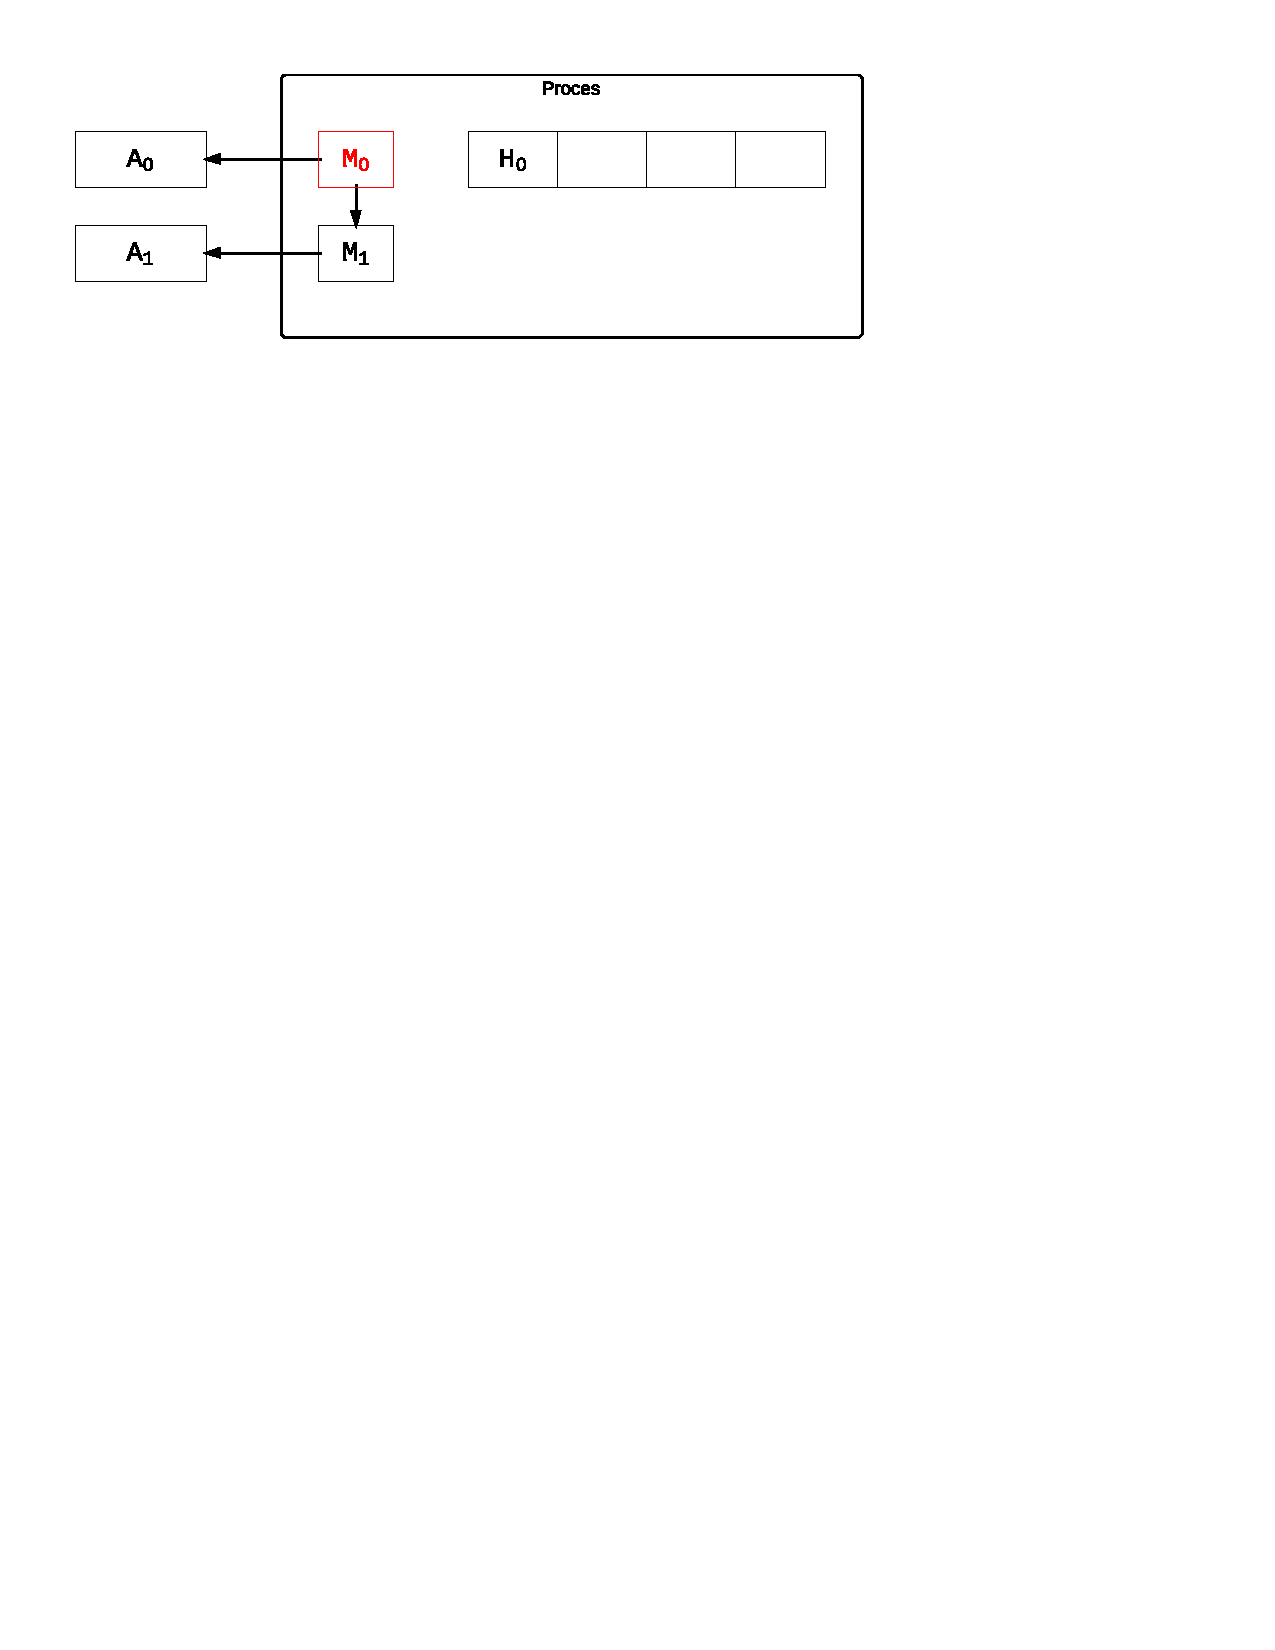
\includegraphics[scale=0.75, clip, trim=10mm 220mm 68mm 10mm]{mp2}}
\caption{Kolejka wiadomości procesu z dodaną kolejną wiadomością.}
\label{fig:mp2}
\end{figure}

W momencie, gdy proces-odbiorca w wykonywanym przez siebie kodzie dochodzi do instrukcji \texttt{loop\_rec} pobierana jest przez niego wiadomość oznaczona wskaźnikiem aktualnej wiadomości. W~sytuacji, gdy kolejka jest pusta proces zostaje zawieszany aż do momentu otrzymania kolejnej wiadomości lub zrealizowania się przeterminowania.
W pierwszym przypadku proces ponownie próbuje pobrać wiadomość z kolejki, w drugim zaś wykonywany jest kod przewidziany po zajściu przeterminowania.

Odebranie wiadomości przez proces polega na skopiowaniu jego zawartości na własną stertę (wyrażenie \textbf{H\textsubscript{1}} na rys. \ref{fig:mp3}), zwolnieniu pamięci zajmowanej przez jej oryginalną zawartość, usunięciu wiadomości z kolejki wiadomości oraz przepisaniu wskaźnika aktualnej wiadomości na następną w kolejce (rys. \ref{fig:mp4}).
Cała procedura jest powtarzana w momencie ponownego dojścia do instrukcji \texttt{loop\_rec} w~kodzie maszynowym (bloku \texttt{receive}).

\begin{figure}[h]
\centerline{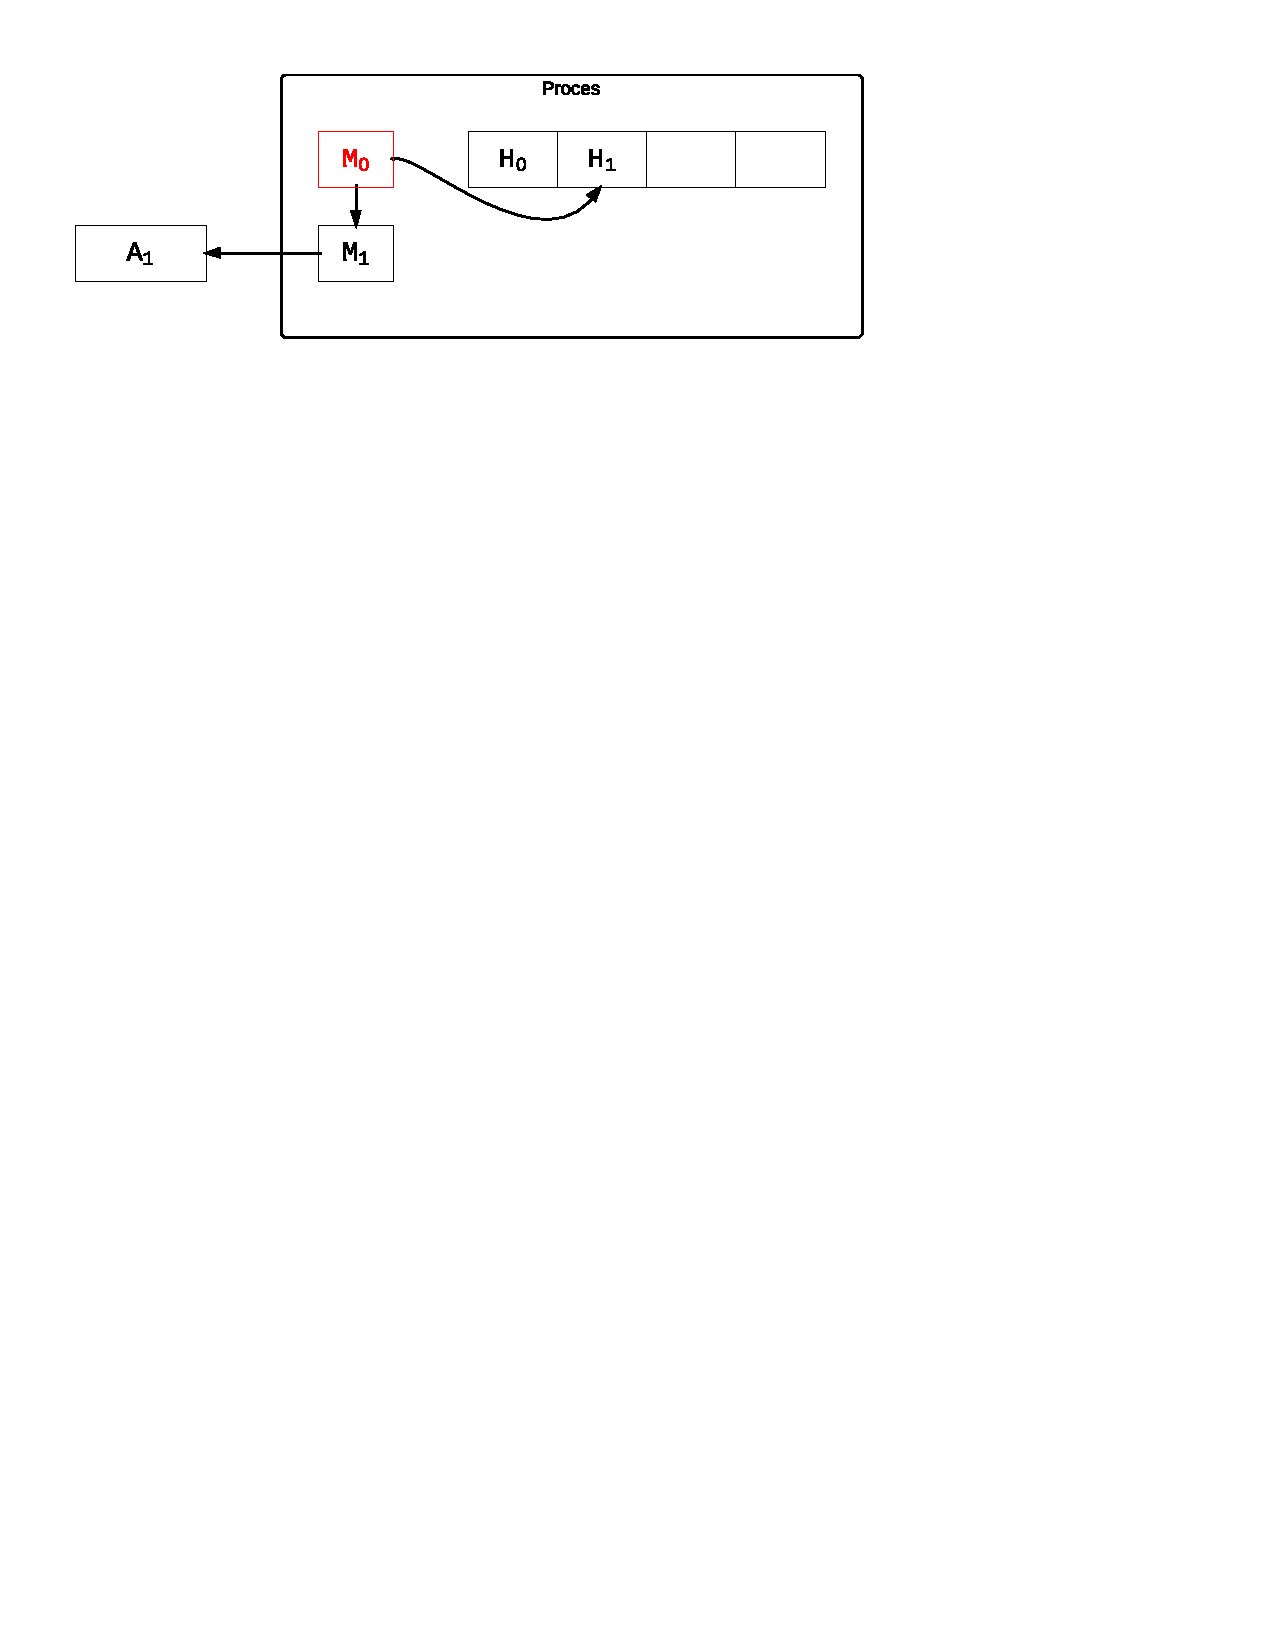
\includegraphics[scale=0.75, clip, trim=10mm 220mm 68mm 10mm]{mp3}}
\caption{Kolejka wiadomości procesu z odczytaną pierwszą wiadomością.}
\label{fig:mp3}
\end{figure}

\begin{figure}[h]
\centerline{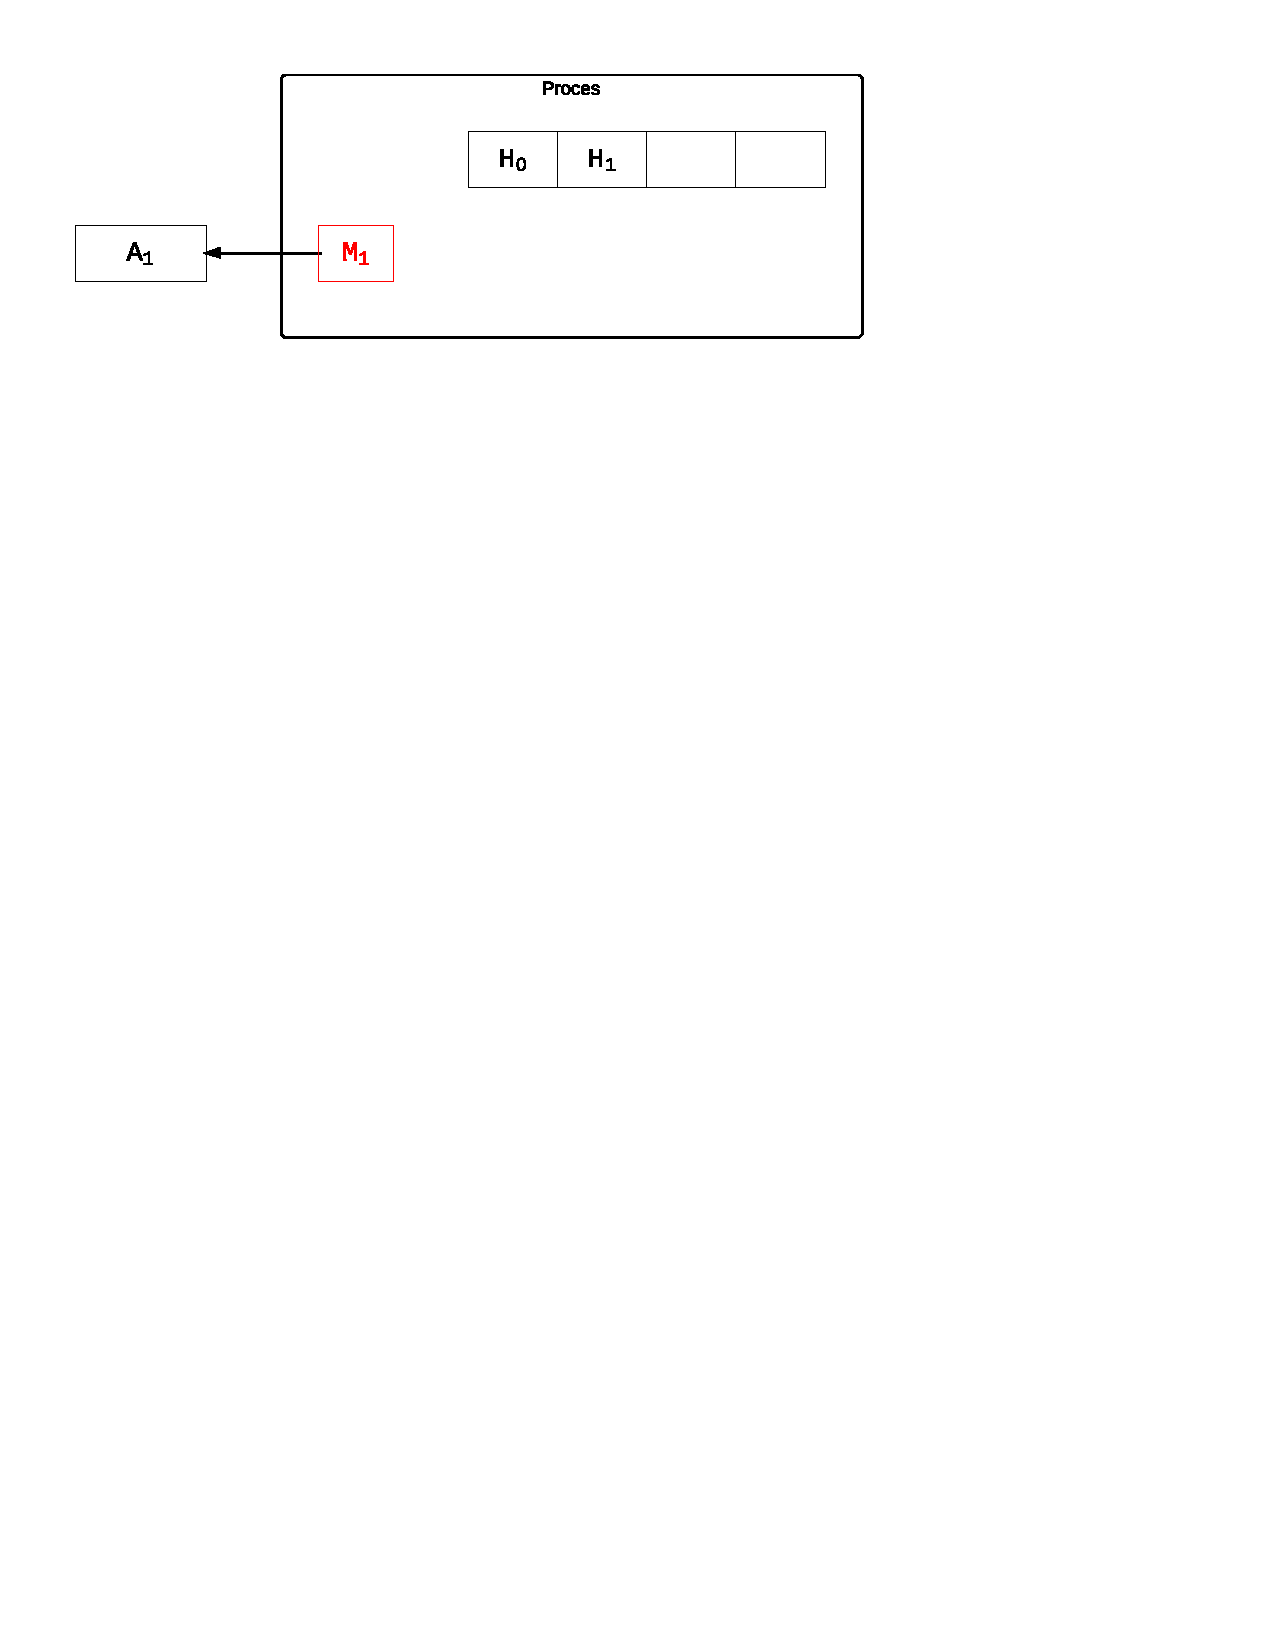
\includegraphics[scale=0.75, clip, trim=10mm 220mm 68mm 10mm]{mp4}}
\caption{Kolejka wiadomości procesu po usunięciu pierwszej wiadomości.}
\label{fig:mp4}
\end{figure}

\subsection{Obsługa błędów}
\label{sub:procBledy}

Maszyna wirtualna opisywana w niniejszej pracy posiada mechanizm dwukierunkowego połączenia procesów (\emph{link}), który zapewnia propagację błędu, w sytuacji gdy w trakcie wykonywania się jednego z~połączonych procesów wystąpi błąd, na skutek którego jego działanie zostanie zakończone.
Domyślnym zachowaniem procesu otrzymującego informację o zakończeniu działania procesu jest w takiej sytuacji jego zakończenie z takim samym błędem.
Możliwe jest jednak ustawienie w nim flagi \texttt{trap\_exit}, czego efektem jest zamiana ww. sygnału na wiadomość wysłaną do tego procesu.

Maszyna wirtualna BEAM oprócz ww. mechanizmu zapewnia również mechanizm jednokierunkowej obserwacji procesów (\emph{monitor}), a także bloki przechwytywania błędów w kodzie (\texttt{try} i \texttt{catch}).
Funkcjonalności te nie zostały jednak zapewnione w maszynie zaimplementowanej w ramach niniejszej pracy.

Lista błędów, jakie mogą wystąpić w trakcie uruchomienia procesu, wraz z opisem sytuacji w jakiej mogą wystąpić została zawarta w dokumentacji języka \cite{ErlangErrors}.

%---------------------------------------------------------------------------
\section{Planista (\emph{scheduler})}
\label{sec:maszynaScheduler}

W systemie współbieżnym procesy mogą działać na jeden z dwóch sposobów:
\begin{itemize}
\item we współbieżności konkurencyjnej (\emph{pre-emptive}), w której planista decyduje o tym kiedy przerwać wykonywanie pewnego procesu i wznowić inne;
\item we współbieżności współpracującej (\emph{cooperative}), w której proces decyduje kiedy przerwać swoje wykonywanie po to, aby \emph{scheduler} mógł wybrać inny proces do wykonania.
\end{itemize}

Z punktu widzenia programisty Erlanga procesy uruchomione w ramach systemu działają we współbieżności konkurencyjnej, gdyż planista sam zarządza kolejką procesów przeznaczonych do wykonania.
Implementacja logiki procesu w maszynie wirtualnej opiera się jednak na współbieżności współpracującej, ponieważ to ona jest odpowiedzialna za wywołanie funkcji wybierającej kolejny proces do wykonania w odpowiedniej chwili. Wynika to z faktu, że wywłaszczenie aktualnie wykonywanego procesu może nastąpić tylko pod pewnymi warunkami.

Pierwszym z nich jest spadek licznika redukcji w danym procesie do zera.
Redukcja jest pojęciem wprowadzonym na potrzeby działania \emph{schedulera} w maszynie wirtualnej BEAM.
Jedna redukcja to wywołanie jednej funkcji (zewnętrznej lub wewnętrznej, operacja z rodziny \textbf{CALL\_*}).
Domyślnie, w maszynie BEAM, gdy \emph{scheduler} wznawia działanie procesu, ten dostaje możliwość wykonania 2000 redukcji zanim będzie musiał oddać dostęp do mocy obliczeniowej innemu procesowi.
W maszynie zaimplementowanej w pracy, ze względu na mniejszą moc obliczeniową docelowej platformy, wartość ta została zmniejszona do 300, podlega ona jednak konfiguracji.
Aby nie doprowadzić do sytuacji, w której można zauważyć znaczącą rozbieżność w czasie dostępu do procesora pomiędzy różnymi procesami, redukcje liczone są także dla innych operacji.
I tak np. funkcje wbudowane czy uruchomienie \emph{garbage collectora} również modyfikują w pewien arbitralny sposób licznik redukcji w procesie. 

Zmiana wykonywanego procesu może wystąpić tylko przed wywołaniem funkcji (czyli przed instrukcją z rodziny \textbf{CALL\_*}), tj. w chwili gdy mamy pewność że wszystkie lokalne zmienne zapisane są na stosie procesu a rejestry \textbf{X} wypełnione są argumentami funkcji.

Procedura zmiany aktualnie wykonywanego procesu polega na odpowiednim zapamiętaniu struktur interpretera w pamięciu procesu przerywającego swoje działanie i odtworzenie tego samego rodzaju danych z pamięciu procesu, który swoje działanie wznawia.
Została ona zaprezentowana na rysunku \ref{fig:preemption}.
Wstrzymywane jest działanie procesu 1, w którego strukturze zapamiętywane są argumenty funkcji którą miał właśnie wywołać.
Zapisywany jest także wskaźnik na szczyt jego stosu oraz wskaźniki instrukcji i~adres powrotu. Na rysunku symbolicznie zostało to oznaczone czerownymi strzałkami.
Proces 2 z kolei wznawia swoje wykonanie. Licznik redukcji zostaje ustawiony ponownie na 300 i wykonywane są operacje odwrotne niż w przypadku procesu 1.
Oznaczone one zostały symbolicznie strzałkami w kolorze zielonym.

\begin{figure}[h]
\centerline{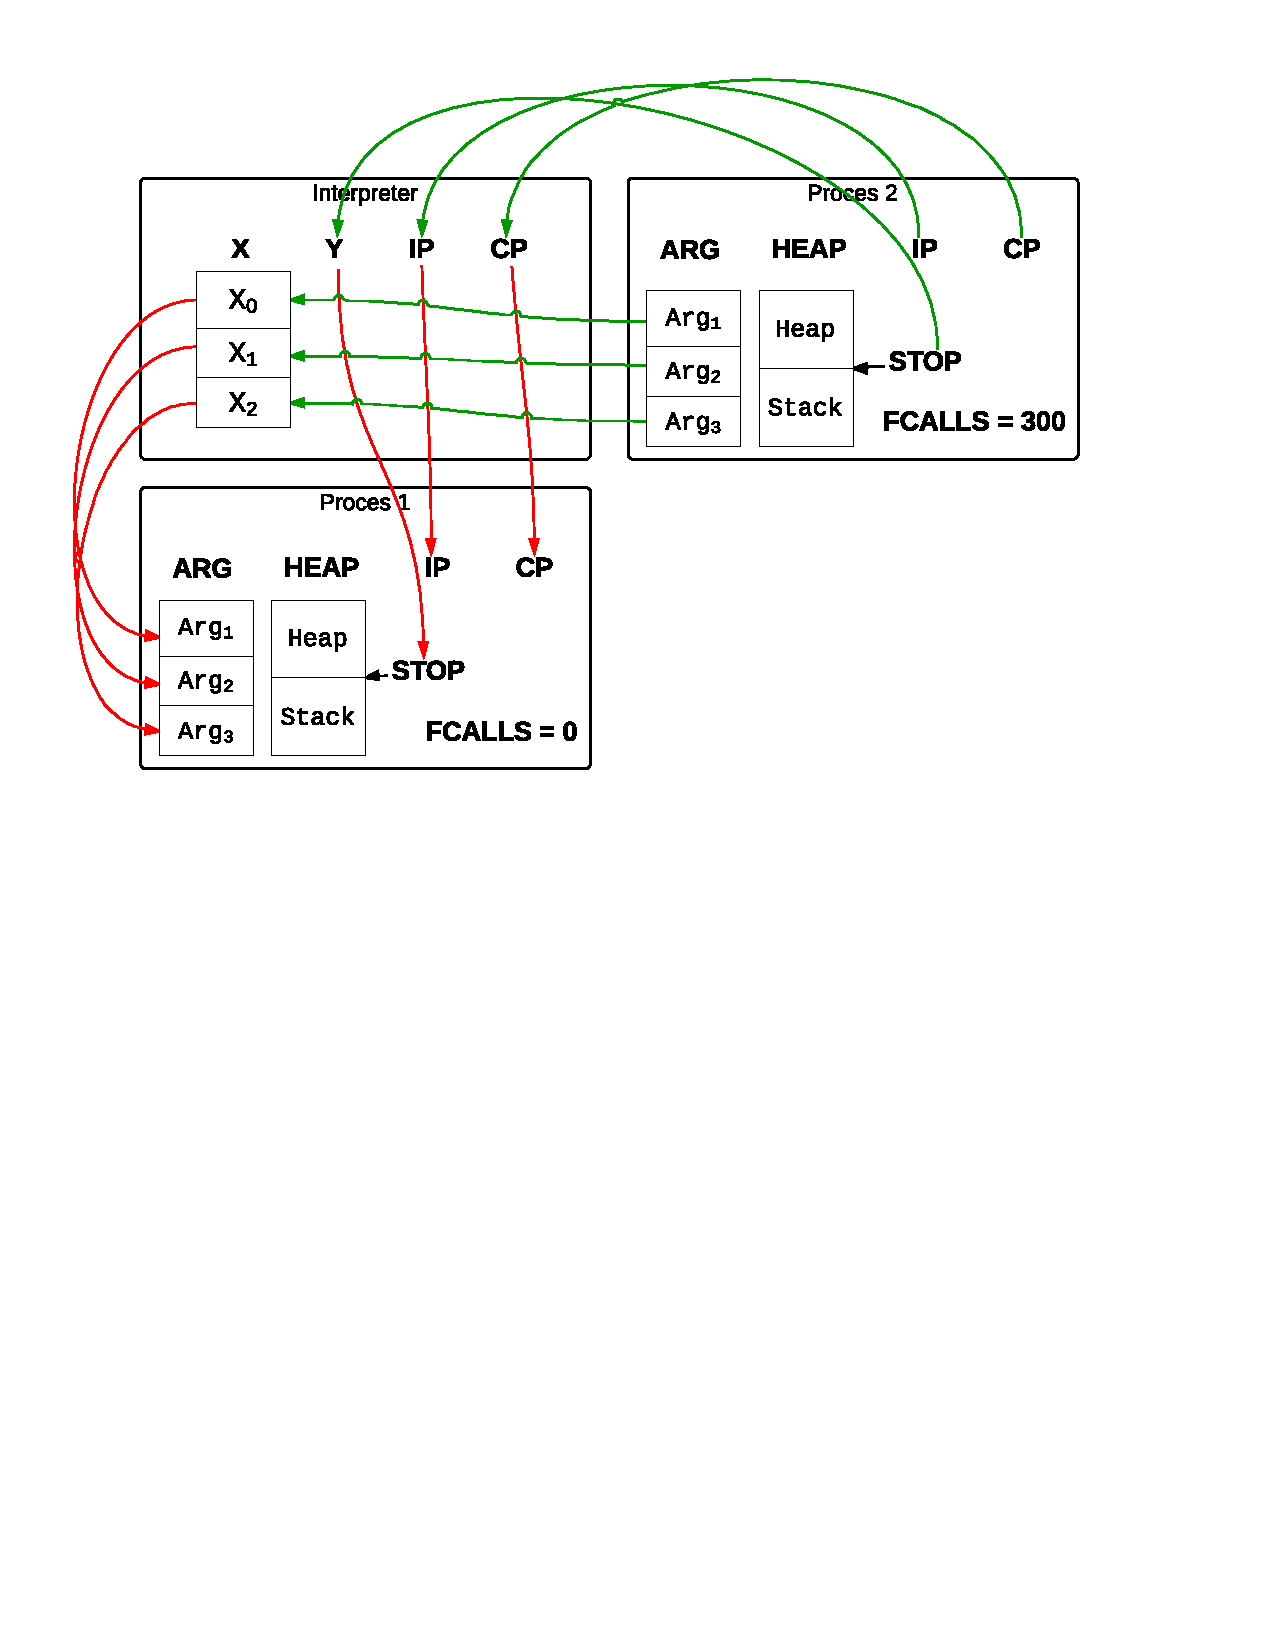
\includegraphics[scale=0.8, clip, trim=10mm 145mm 30mm 10mm]{preemption}}
\caption{Operacje wykonywane w trakcie zmiany wykonywanego procesu}
\label{fig:preemption}
\end{figure}

Istnieje możliwość uruchomienia maszyny wirtualnej BEAM w architekturze SMP (\emph{Symmetric Multiprocessing}), co domyślnie powoduje uruchomienie jednej instancji \emph{schedulera} na jednym fizycznym wątku procesora.
Synchronizację między planistami zapewniają w niej skomplikowane mechanizmy będące przedmiotem ciągłej optymalizacji.
Maszynę zaimplementowaną w pracy można uruchomić jednak tylko z~wykorzystaniem tylko jednego fizycznego wątku.
Pomimo badań nad uruchomieniem \emph{schedulera} mikrojądra FreeRTOS na architekturze wielordzeniowej \cite{Mistry2011}, oficjalna dystrybucja wspiera obecnie tylko architekturę jednordzeniową.

Maszyna wirtualna BEAM posiada zaimplementowane priorytety procesów: \textbf{max}, \textbf{high}, \textbf{normal} oraz \textbf{low}.
Procesy domyślnie uruchomiane są z priorytetem \textbf{normal}. 
Planista, w momencie gdy licznik redukcji aktualnie wykonywanego procesu osiągnie wartość 0 lub proces będzie oczekiwał na wiadomość w bloku \texttt{receive}, dokona wyboru kolejnego procesu do wykonania.

Proces może zostać wybrany spośród trzech dostępnych kolejek zawierających procesy o priorytecie:
\begin{itemize}
\item \textbf{max} --- jeżeli w kolejce jest zakolejkowany przynajmniej jeden proces to jest będzie on wybranym jako kolejny do wykonania;
\item \textbf{high} --- jeżeli kolejka procesów o priorytecie \textbf{max} jest pusta a w tej kolejce znajduje się przynajmniej jeden proces to zostanie on wybrany do uruchomienia;
\item \textbf{normal} i \textbf{low} --- kolejka zawiera procesy o dwóch priorytetach, jednak procesy o priorytecie \textbf{low} zawierają specjalny licznik, który wskazuje na to ile razy proces musi zostać pominięty przy wyborze do uruchomienia zanim faktycznie zostanie uruchomiony. Wartość licznika dla tego rodzaju procesów po zakolejkowaniu wynosi 8. Procesy z tej kolejki mogą zostać wybrane do wznowienia przez \emph{scheduler} tylko w sytuacji gdy kolejki z procesami o priorytetach \textbf{max} i \textbf{high} są puste.
\end{itemize}

Aktualny proces umieszczany jest na końcu kolejki odpowiadającej swojemu priorytetowi od razu (jeżeli zostaje zatrzymany z powodu wyczerpania się dostępnych redukcji) lub po otrzymaniu wiadomości lub przeterminowaniu (jeśli został zatrzymany na skutek wejścia w blok \texttt{receive}).

Wersja maszyny wirtualnej zaimplementowanej w pracy nie implementuje możliwości zmiany priorytetu uruchomionego procesu.
Wszystkie procesy uruchamiane są z takim samym priorytetem.
Jest to jednak funkcjonalność, której implementacja jest godna rozważenia w trakcie dalszego rozwoju projektu, biorąc pod uwagę fakt, że mikrojądro FreeRTOS pozwala na wybór priorytetu zadania a działanie planisty systemu jest bardzo podobne do ww. mechanizmu działania \emph{schedulera} maszyny wirtualnej BEAM.

%---------------------------------------------------------------------------
\section{Funkcje wbudowane (\emph{Built-In Functions})}
\label{sec:maszynaBIF}

W niniejszym podrozdziale zaprezentowano zbiór zaimplementowanych funkcji wbudowanych w~maszynę wirtualną dla systemu FreeRTOS.
Z punktu widzenia programisty funkcja wbudowana jest zwykłą funkcją zaimplementowaną w zewnętrznym module, jej implementacja jest jednak częścią kodu maszyny wirtualnej w języku C.
Nie jest zatem wykonywana ona jako kod pośredni przez interpreter, ale jako kod maszynowy danej architektury, co wpływa pozytywnie na szybkość jej wykonania.
Każdej funkcji wbudowanej odpowiada wpis w tablicy funkcji eksportowanych, podobnie jak funkcjom eksportowanym z załadowanych modułów.
Wpis ten zamiast wskaźnika do instrukcji kodu maszynowego do wykonania zawiera wskaźnik do funkcji zaimplementowanej w języku C.

\subsection{Funkcje ogólne (moduł \texttt{erlang})}
\label{sub:bifErlang}
Funkcje opisane w tej części podrozdziału zostały zaimplementowane w pliku źródłowym \texttt{erl\_bif.c}.

\begin{longtable}{|c|c|p{7.5cm}|}
\hline

Funkcja & Argumenty & Opis \\
\endfirsthead
\hline
\texttt{splus/2} & \texttt{Arg1 Arg2} & Zwraca \texttt{Arg1 + Arg2} \\
\hline
\texttt{sminus/2} & \texttt{Arg1 Arg2} & Zwraca \texttt{Arg1 - Arg2} \\
\hline
\texttt{stimes/2} & \texttt{Arg1 Arg2} & Zwraca \texttt{Arg1 * Arg2} \\
\hline
\texttt{spawn/3} & \texttt{M F A} & Startuje nowy proces, wykonujący funkcję \texttt{F} w~module \texttt{M} z listą argumentów \texttt{A} \\
\hline
\texttt{spawn\_link/3} & \texttt{M F A} & Startuje nowy proces, wykonujący funkcję \texttt{F} w~module \texttt{M} z listą argumentów \texttt{A}. Łączy wystartowany proces z wywołującym \emph{linkiem}.\\
\hline
\texttt{setelement/3} & \texttt{Index Tuple Element} & Zwraca nową krotkę, taką jak \texttt{Tuple}, ale z elementem \texttt{Element} na pozycji \texttt{Index} \\
\hline
\texttt{now/0} & & Zwraca krotkę \texttt{\{M,S,U\}} zawierająca kolejną liczbę megasekund, sekund i mikrosekund jakie upłynęły od uruchomienia maszyny wirtualnej \\
\hline
\texttt{length/1} & \texttt{List} & Zwraca długość listy \texttt{List} \\
\hline
\texttt{plusplus/2} & \texttt{List1 List2} & Zwraca nową listę, stanowiącą złączenie list \texttt{List1} i \texttt{List2} \\
\hline
\texttt{div/2} & \texttt{Int1 Int2} & Zwraca wynik dzielenia całkowitoliczbowego argumentów \\
\hline
\texttt{rem/2} & \texttt{Int1 Int2} & Zwraca resztę z dzielenia argumentów \\
\hline
\texttt{bsr/2} & \texttt{Int1 Int2} & Zwraca wynik przesunięcia bitowego w prawo argumentów \\
\hline
\texttt{band/2} & \texttt{Int1 Int2} & Zwraca iloczyn logiczny argumentów \\
\hline
\texttt{bor/2} & \texttt{Int1 Int2} & Zwraca alternatywę logiczną argumentów \\
\hline
\texttt{element/2} & \texttt{N Tuple} & Zwraca \texttt{N}-ty element krotki \texttt{Tuple} \\
\hline
\texttt{exit/1} & \texttt{Reason} & Kończy działanie wywołującego procesu z powodem \texttt{Reason} \\
\hline
\texttt{process\_flag/2} & \texttt{trap\_exit true} & Wywołujący proces nie kończy działania gdy kończą działania procesy połączone, ale otrzymuje informacje o tym fakcie w postaci wiadomości \\
\hline
\texttt{self/0} & & Zwraca \textbf{PID} wywołującego procesu \\
\hline
\texttt{send\_after/3} & \texttt{Time Dest Mesg} & Ustawia przeterminowanie wysyłające wiadomość \texttt{Mesg} do procesu \texttt{Dest} za \texttt{Time} milisekund. \\
\hline
\caption{Zaimplementowane funkcje wbudowane w module \texttt{erlang}} 
\label{table:bifErlang} \\
\end{longtable}


\subsection{Listy (moduł \texttt{lists})}
\label{sub:bifLists}

Funkcje opisane w tej części podrozdziału zostały zaimplementowane w pliku źródłowym \texttt{erl\_bif\_lists.c}.

\begin{longtable}{|c|c|p{8cm}|}
\hline

Funkcja & Argumenty & Opis \\
\endfirsthead
\hline
\texttt{reverse/1} & \texttt{List} & Zwraca nową listę bedącą odwróconą listą \texttt{List} \\
\hline
\caption{Zaimplementowane funkcje wbudowane w module \texttt{lists}} 
\label{table:bifLists} \\
\end{longtable}

\subsection{GPIO i obsługa przerwań (moduł \texttt{lpc\_gpio})}
\label{sub:bifGPIO}
Funkcje opisane w tej części podrozdziału zostały zaimplementowane w pliku źródłowym \texttt{erl\_bif\_lpc.c}.

\begin{longtable}{|c|c|p{10cm}|}
\hline

Funkcja & Argumenty & Opis \\
\endfirsthead
\hline
\texttt{output/2} & \texttt{Port Pin} & Ustawia pin \texttt{Pin} na porcie \texttt{Port} mikrokontrolera w tryb wyjścia\\
\hline
\texttt{high/2} & \texttt{Port Pin} & Ustawia stan wysoki na pinie \texttt{Pin} na porcie \texttt{Port} \\
\hline
\texttt{low/2} & \texttt{Port Pin} & Ustawia stan niski na pinie \texttt{Pin} na porcie \texttt{Port} \\
\hline
\texttt{interrupt/3} & \texttt{0 Pin falling} & Subskrybuje proces na opadające zbocze na pinie \texttt{Pin} na porcie \texttt{0}. Informacja  o przerwaniu dotrze do procesu w postaci wiadomości w postaci \texttt{interrupt}.\\
\hline
\caption{Zaimplementowane funkcje wbudowane w module \texttt{lpc\_gpio}} 
\label{table:bifGpio} \\
\end{longtable}


\subsection{SPI (moduł \texttt{lpc\_spi})}
\label{sub:bifSPI}

Funkcje opisane w tej części podrozdziału zostały zaimplementowane w pliku źródłowym \texttt{erl\_bif\_spi.c}.

\begin{longtable}{|c|c|p{10cm}|}
\hline

Funkcja & Argumenty & Opis \\
\endfirsthead
\hline
\texttt{init/1} & \texttt{Frequency} & Inicjalizuje interfejs SPI mikrokontrolera w trybie \emph{master} z sygnałem zegarowym o częstotiwości \texttt{Frequency} \\
\hline
\texttt{rw/1} & \texttt{Byte} & Wysyła bajt \texttt{Byte} po interfejsie SPI. Wartością zwracaną jest bajt otrzymany z interfejsu w trakcie transmisji. \\
\hline
\caption{Zaimplementowane funkcje wbudowane w module \texttt{lpc\_spi}} 
\label{table:bifSpi} \\
\end{longtable}

\subsection{Funkcje pomocnicze (moduł \texttt{lpc\_debug})}
\label{sub:bifDebug}
Funkcje opisane w tej części podrozdziału zostały zaimplementowane w pliku źródłowym \texttt{erl\_bif\_lpc.c}.

\begin{longtable}{|c|c|p{10cm}|}
\hline

Funkcja & Argumenty & Opis \\
\endfirsthead
\hline
\texttt{dump\_regs/0} &  & Drukuje zawartość rejestrów X\\
\hline
\texttt{dump\_stack/0} &  & Drukuje zawartość stosu wywołującego procesu\\
\hline
\texttt{dump\_heap/0} &  & Drukuje zawartość sterty wywołującego procesu\\
\hline
\texttt{print\_info/0} &  & Drukuje informacje dotyczące wywołującego procesu\\
\hline
\texttt{print\_term/1} & \texttt{Term}  & Drukuje zawartość wyrażenia \texttt{Term} \\
\hline
\caption{Zaimplementowane funkcje wbudowane w module \texttt{lpc\_debug}} 
\label{table:bifDebug} \\
\end{longtable}

%---------------------------------------------------------------------------
\section{\emph{Garbage collector}}
\label{sec:maszynaGC}

Moduł opisany w niniejszym podrozdziale został zaimplementowany w pliku źródłowym \texttt{erl\_gc.c}.

\subsection{Pamięć zajmowana przez proces}
\label{sub:gcHeap}

Blok pamięci zajmowany przez proces do przechowywania wyrażeń których używa nosi nazwę sterty i zarządzany jest automatycznie przez \emph{garbage collector}.
Obszar pamięci ten podzielony jest na dwie części:
\begin{itemize}
\item stertę, służącą do przechowywania danych złożonych (krotki, listy) lub opakowanych (\textbf{BOXED}), z których proces może korzystać nawet przez cały czas swojego życia;
\item stos, którego zadaniem jest zachowywanie informacji pomiędzy wywołaniami funkcji, takich jak zmienne lokalne czy adresy powrotu.
\end{itemize}

Pojęcie sterty jest w niniejszej pracy używane wymiennie w odniesieniu albo do całego zaalokowanego dla procesu bloku pamięci albo do pierwszej wspomnianej jego części.
Proces przechowuje kilka wskaźników dzięki którym możliwa jest identyfikacja odpowiednich fragmentów pamięci i wykonywanie operacji na nich. Należą do nich:
\begin{itemize}
\item \textbf{HEAP}, oznaczający początek całego bloku pamięci, a zarazem i sterty;
\item \textbf{HTOP}, oznaczający koniec sterty;
\item \textbf{STOP}, oznaczający początek stosu;
\item \textbf{HEND}, oznaczający koniec bloku pamięci, a zarazem i stosu.
\end{itemize}
Graficzne odniesienie wskaźników do miejsc w pamięci procesu zostało zaprezentowane na rysunku \ref{fig:heap}. 
Jak można zauważyć, wyrażenia dodawane do sterty procesu umieszczane są począwszy od początku całego bloku pamięci.
Z kolei wyrażenia dodawane na stos umieszczane są od końca bloku, w~kierunku jego początku.
Wskazywanie przez wskaźniki \textbf{HTOP} oraz \textbf{STOP} na to samo miejsce w~pamięci oznacza, że na stercie procesu skończyło się miejsce i konieczne jest uruchomienie \emph{garbage collectora}.

\begin{figure}[h]
\centerline{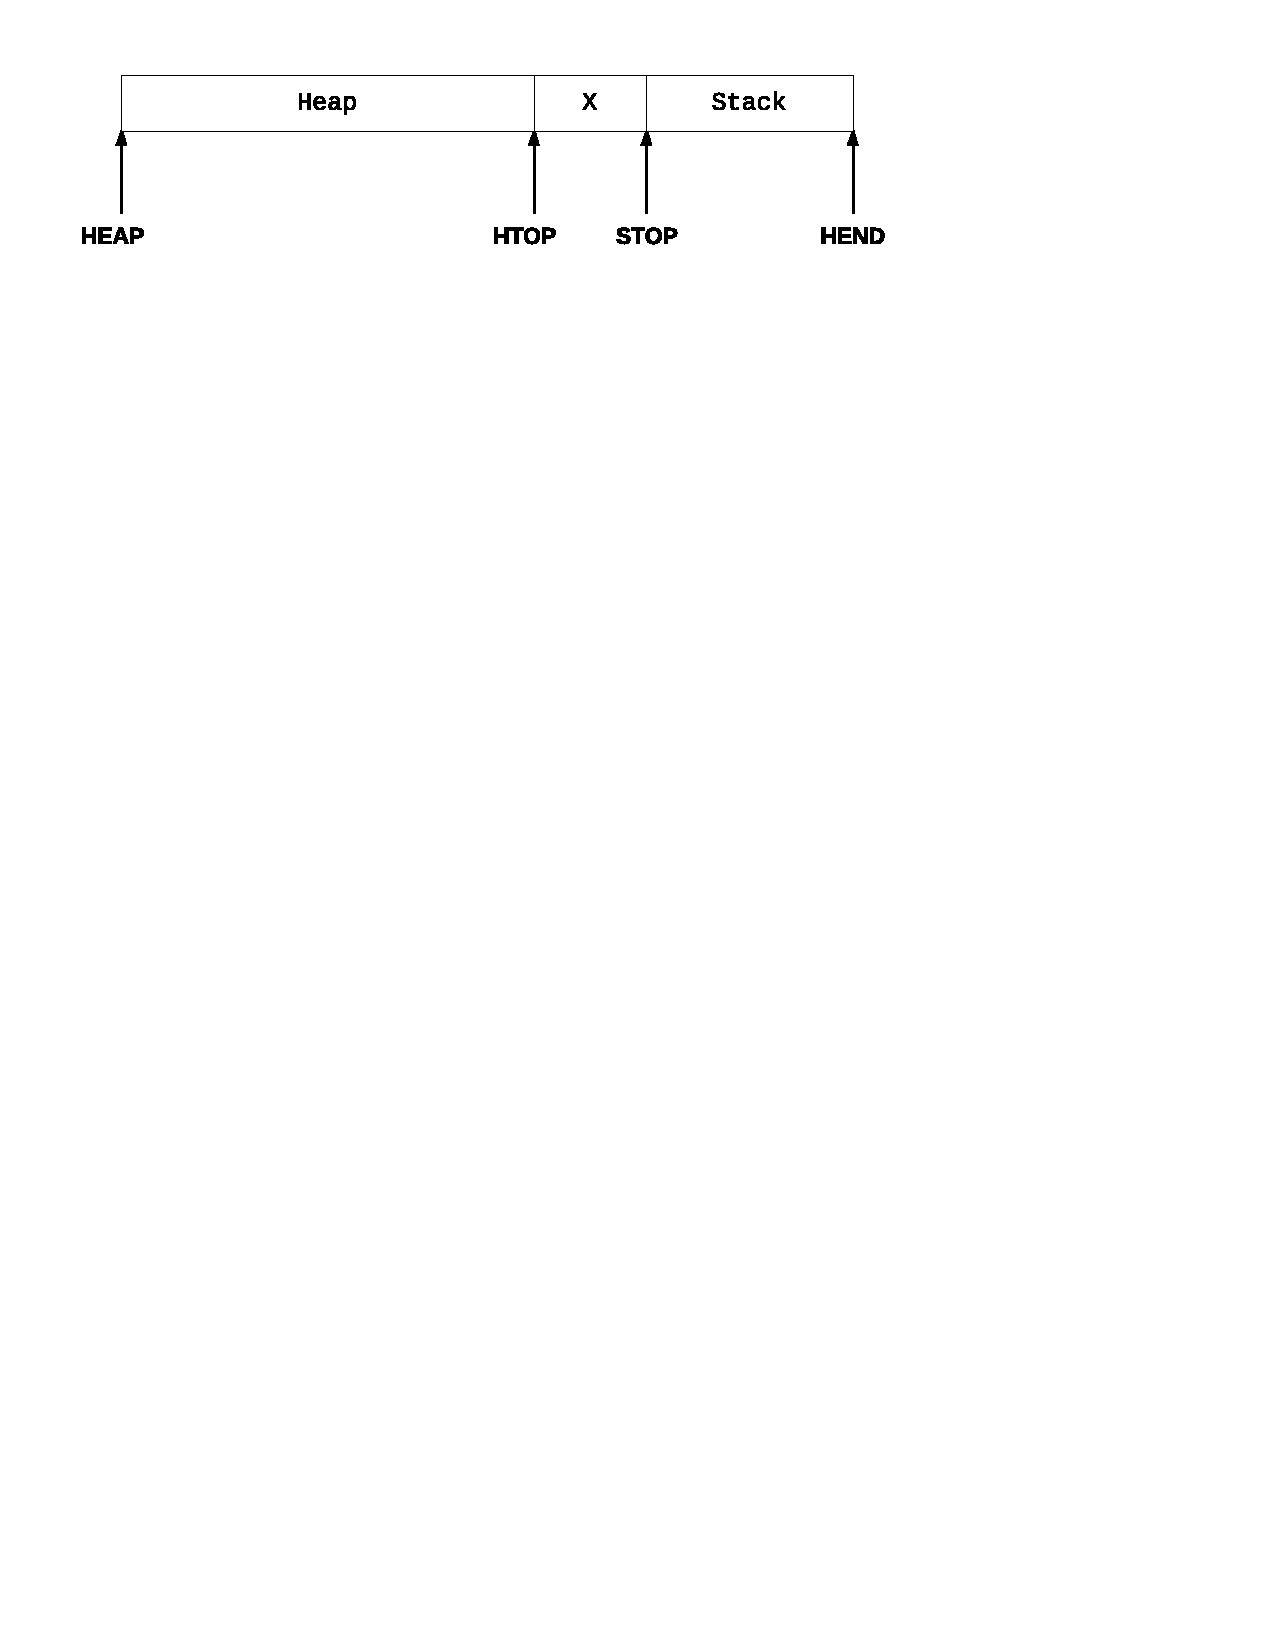
\includegraphics[scale=1, clip, trim=10mm 235mm 65mm 10mm]{heap}}
\caption{Struktura pamięci zajmowanej przez proces wraz ze wskaźnikami na poszczególne struktury}
\label{fig:heap}
\end{figure}

Sterta zaalokowana dla procesu może mieć jeden z pewnych ustalonych z góry rozmiarów, należący do ciągu:

\begin{equation}
h_{n} = \left\lbrace
\begin{array}{rcl}
12 & \text{dla} & n = 1,\\
38 & \text{dla} & n = 2,\\
h_{n-1} + h_{n-2} + 1 & \text{dla} & n > 2
\end{array}
\right.
\end{equation}

Rozmiar ten wyrażony jest w słowach maszynowych i dla maszyny BEAM domyślnie wynosi 233 (6. wyraz ciągu).
W maszynie zaimplementowanej w pracy domyślnym, początkowym rozmiarem sterty procesu jest 12 słów maszynowych ze względu na mniejsze zapotrzebowanie na pamięć, wynikające~z~przeznaczenia aplikacji.

\subsection{Algorytm Cheneya}
\label{sub:gcCheney}

Algorytmem odśmiecania wykorzystywanym w maszynie wirtualnej Erlanga jest algorytm Cheneya \cite{Cheney1970}.
Jest on algorytmem kopiującym, którego działanie polega na zaalokowaniu nowego bloku pamięci i przeniesieniu do niego wszystkich obecnie używanych obiektów.
Kolejnym krokiem jest przepisanie wszystkich istniejących referencji do poprzedniego bloku pamięci.
Na końcu następuje zwolnienie starego bloku pamięci.
Ten prosty algorytm pasuje do filozofii języka, gdzie każdy uruchomiony proces korzysta tylko i wyłącznie z pamięci zajmowanej przez samego siebie.
Dzięki temu możliwe jest uruchamianie \emph{garbage collectora} w kontekście każdego procesu z osobna.
Nie powoduje to zatrzymań działania całego uruchomionego systemu na czas odśmiecania sterty procesu.
Algorytm zostanie uruchomiony w~sytuacji, gdy na stercie nie ma wolnej liczby słów maszynowych potrzebnej do zaalokowania w danej chwili lub zostanie on wywołany \emph{explicite} przez funkcję \texttt{erlang:garbage\_collect/0-2}.

Działanie algorytmu Cheneya uruchomionego w procesie erlangowego zostało zaprezentowano na rysunkach od \ref{fig:gc0} do \ref{fig:gc6}.
Do zilustrowania sposobu działania algorytmu posłużono się abstrakcją trójkolorową, służącą do znalezienia obiektów których pamięć można zwolnić, wykorzystującą do ich oznaczania trzech kolorów:
\begin{itemize}
\item białego, oznaczającego że stan obiektu jest w tym momencie nieznany, ale nie napotkano jeszcze żadnego obiektu odwołującego się do niego;
\item szarego, obiekt jest wykorzystywany i nie można go usunąć, ale nie przetworzono jeszcze obiektów zależnych od niego;
\item czarnego, obiekt, podobnie jak obiekty od niego zależne, są wykorzystywane.
\end{itemize}
Celem algorytmu odśmiecania jest osiągnięcie takiego stanu, w którym wszystkie obiekty będą oznaczone kolorem czarnym (obiekty wykorzystywane) lub białym (obiekty niewykorzystywane które można usunąć z pamięci).
Na początku działania algorytmu, początkowy zbiór wyrażeń oznaczony jest kolorem szarym.
Ze względu na kopiujący charakter algorytmu, kolor obiektów na dotychczasowej stercie procesu będzie zawsze biały.
Obiekty przekopiowane na nową stertę będą z kolei tylko szare lub czarne.

Do początkowego zbioru wyrażeń, które odnosić będą się do używanej pamięci, w zaimplementowanej maszynie należą:
stos procesu, używane rejestry \textbf{X} i kolejka wiadomości (rys. \ref{fig:gc0}). W maszynie wirtualnej BEAM do tego zbioru należy jeszcze kilka innych struktur, jak np. słownik procesu.

\begin{figure}[h]
\centerline{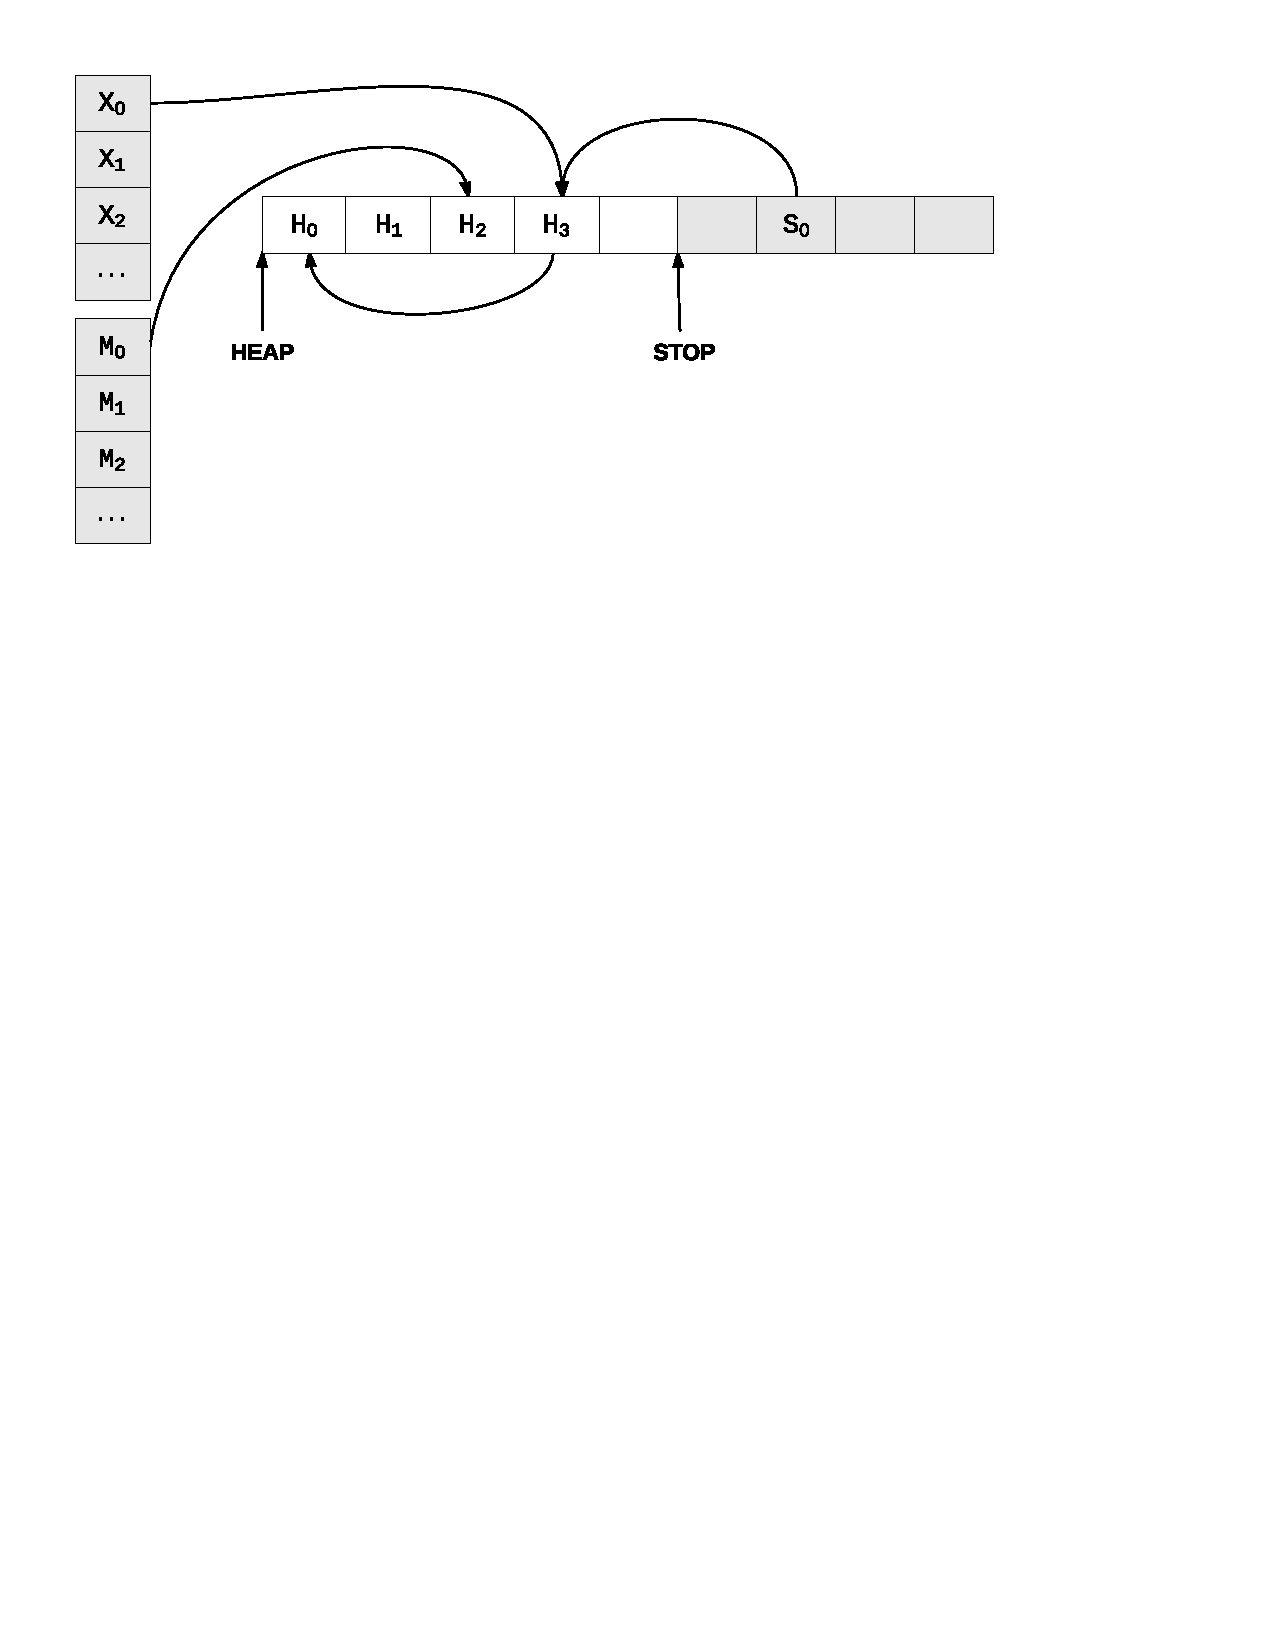
\includegraphics[scale=0.75, clip, trim=10mm 185mm 45mm 10mm]{gc_0}}
\caption{Sterta poddawana odśmiecaniu. Szary zbiór stanowi stos procesu, rejestry \textbf{X} i kolejka wiadomości procesu.}
\label{fig:gc0}
\end{figure}

Pierwszym krokiem działania algorytmu jest zaalokowanie sterty procesu o takiej samej długości jak dotychczasowa (rys. \ref{fig:gc1}).
Następnie przetwarzane są kolejne elementy zbioru szarego, a wyrażenia do których zawierają referencję kopiowane są na nową stertę.
Tak jest w przypadku wyrażenia \textbf{H\textsubscript{3}}, do którego odnosi się rejestr \textbf{X\textsubscript{0}}.
Wyrażenie to zostało przekopiowane na nową stertę i referencja do nowego wyrażenia została zapisana w tym rejestrze.
Obiekt \textbf{H\textsubscript{3}'} miał w tym momencie kolor szary.
Dlatego, że on sam zawierał referencję do wyrażenia \textbf{H\textsubscript{0}}, to wyrażenie także musiało zostać przeniesione na nową stertę.
Przeniesiony obiekt nie zawierał już referencji do żadnego innego obiektu, dlatego zaraz po oznaczeniu go kolorem szarym można było zmienić jego kolor na czarny.

\begin{figure}[h]
\centerline{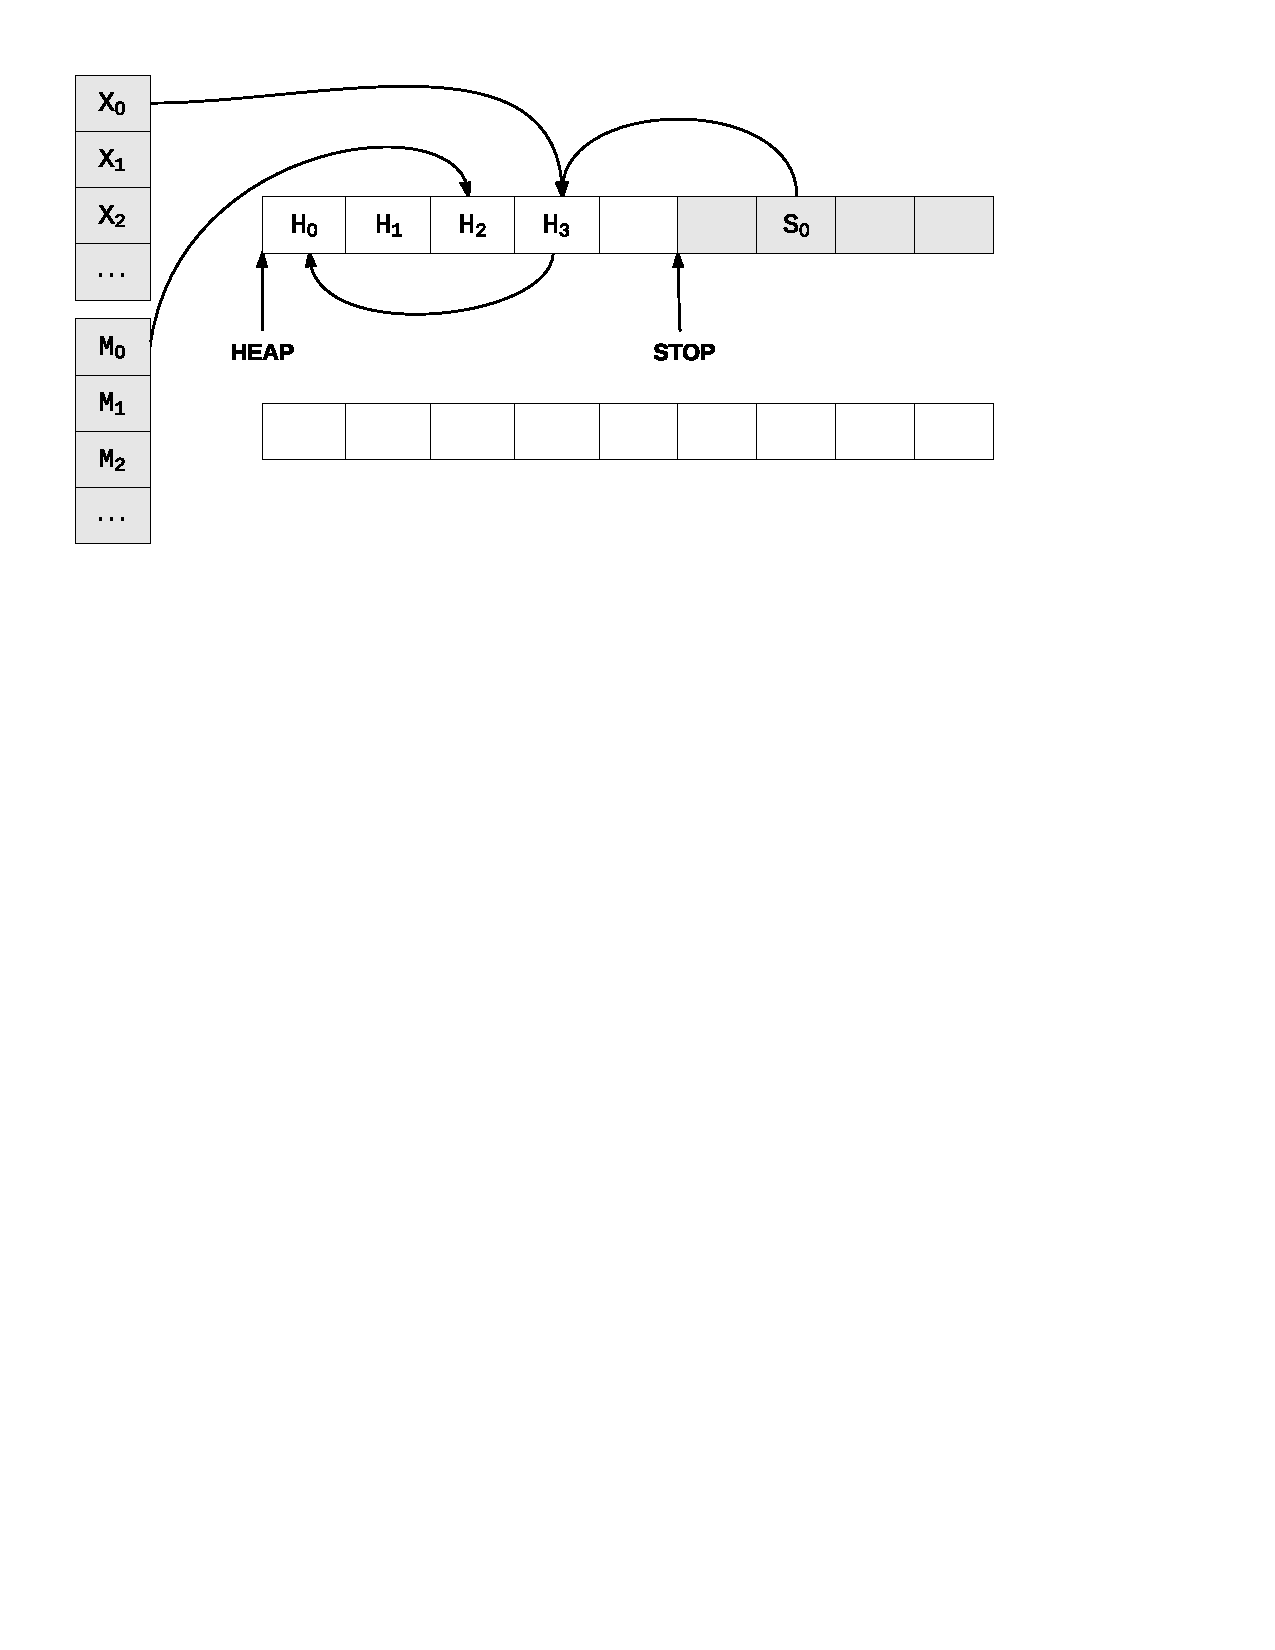
\includegraphics[scale=0.75, clip, trim=10mm 185mm 45mm 10mm]{gc_1}}
\caption{Alokacja nowej sterty o takim samym rozmiarze jak dotychczasowa.}
\label{fig:gc1}
\end{figure}

Dopiero po podmianie referencji w~wyrażeniu \textbf{H\textsubscript{3}'} do obiektu \textbf{H\textsubscript{0}'} można było oznaczyć ten pierwszy kolorem czarnym (rys. \ref{fig:gc2}).
Należy również zauważyć, że staremu obiektowi \textbf{H\textsubscript{3}} przypisano jego kopię na nowej stercie.
Zabieg ten wykonany został po to, aby kolejne obiekty ze zbioru szarego odnoszące się do niego nie kopiowały go na nową stertę, ale zaktualizowały referencję do jego istniejącej już kopii.

\begin{figure}[h]
\centerline{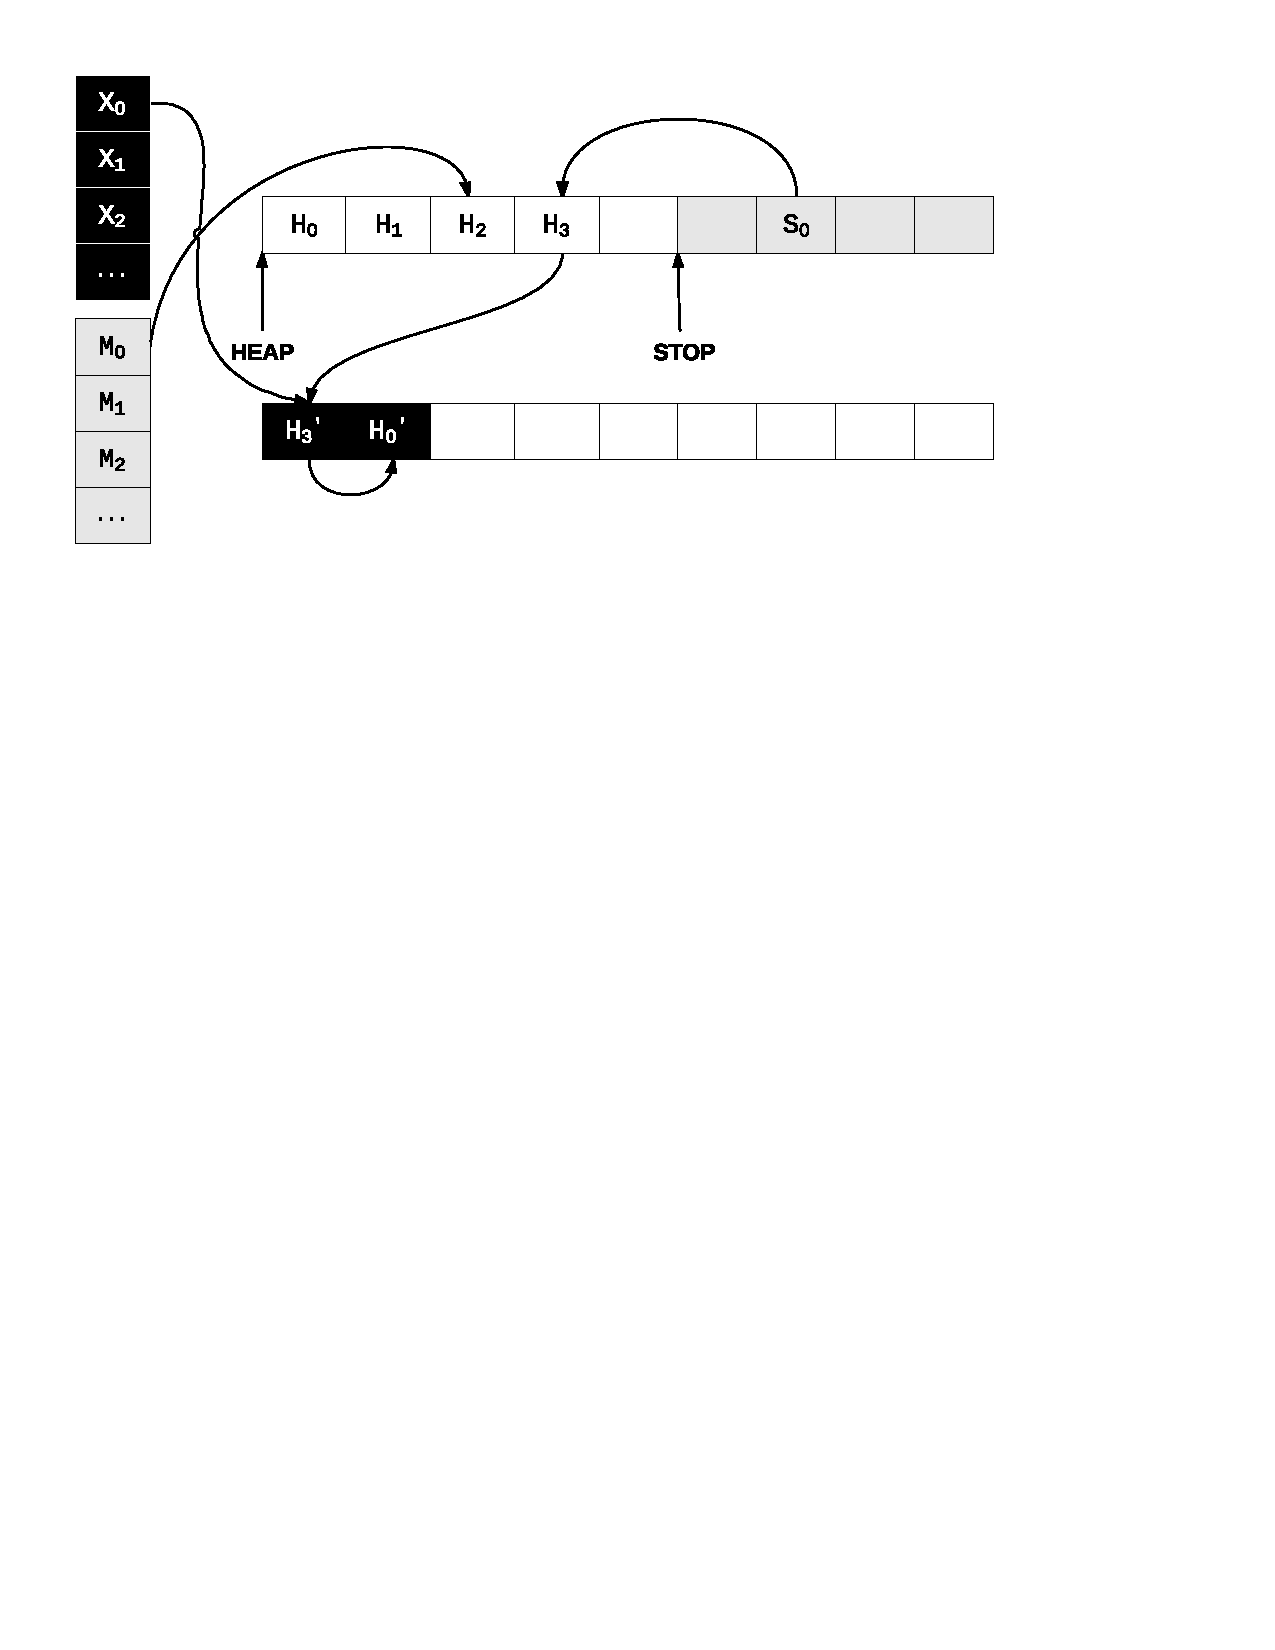
\includegraphics[scale=0.75, clip, trim=10mm 185mm 45mm 10mm]{gc_2}}
\caption{Przeniesienie wyrażeń mających źródło w rejestrach na nową stertę.}
\label{fig:gc2}
\end{figure}

Analogicznie, na nową stertę przeniesione zostało wyrażenie \textbf{H\textsubscript{2}}, do którego odnosiła się wiadomość \textbf{M\textsubscript{0}} (rys. \ref{fig:gc3}).

\begin{figure}[h]
\centerline{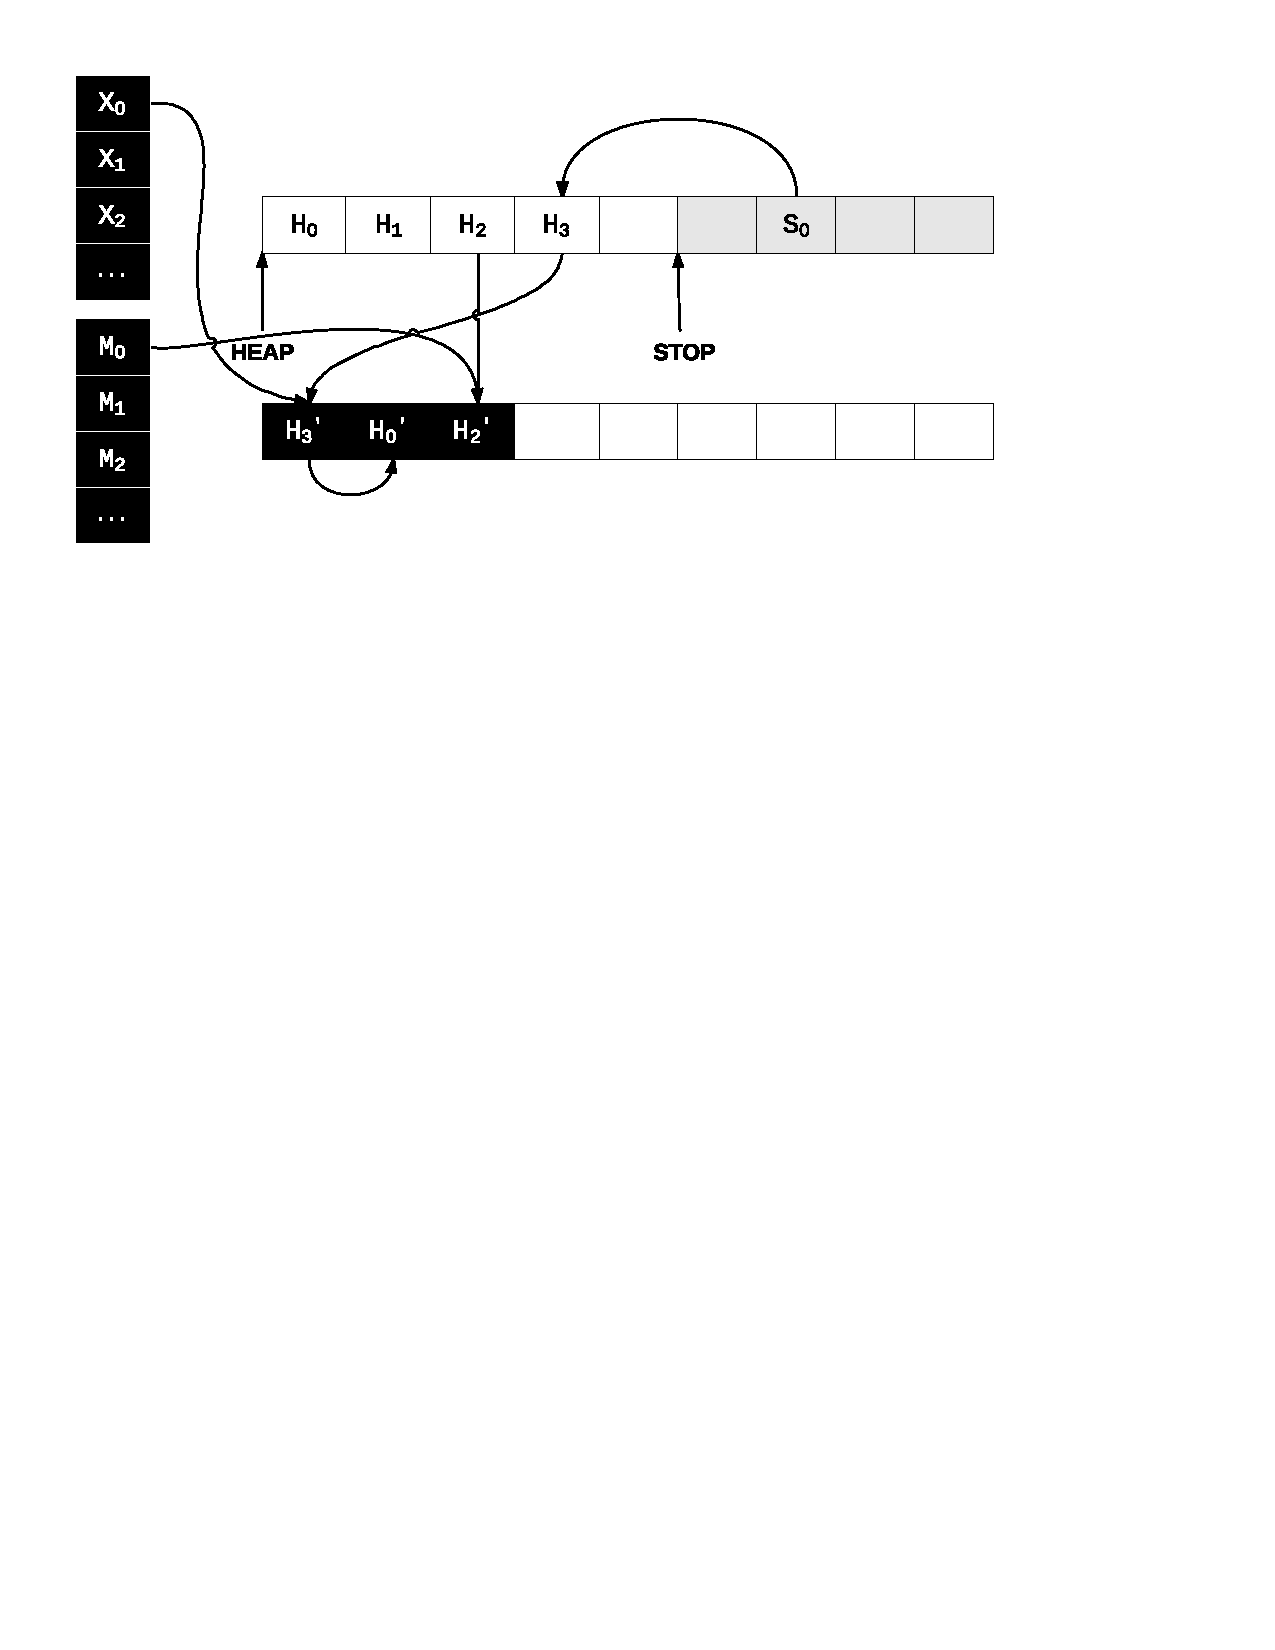
\includegraphics[scale=0.75, clip, trim=10mm 185mm 45mm 10mm]{gc_3}}
\caption{Przeniesienie wyrażeń mających źródło w kolejce wiadomości.}
\label{fig:gc3}
\end{figure}

Ostatnim analizowanym zbiorem szarym był stos procesu, w którym wyrażenie \textbf{S\textsubscript{0}} odnosiło się do, przeniesionego już wcześniej, wyrażenia \textbf{H\textsubscript{0}}. Dlatego też w tym kroku wystarczające było przepisanie referencji do kopii tego obiektu do wyrażenia na stosie (rys. \ref{fig:gc4}).

\begin{figure}[h]
\centerline{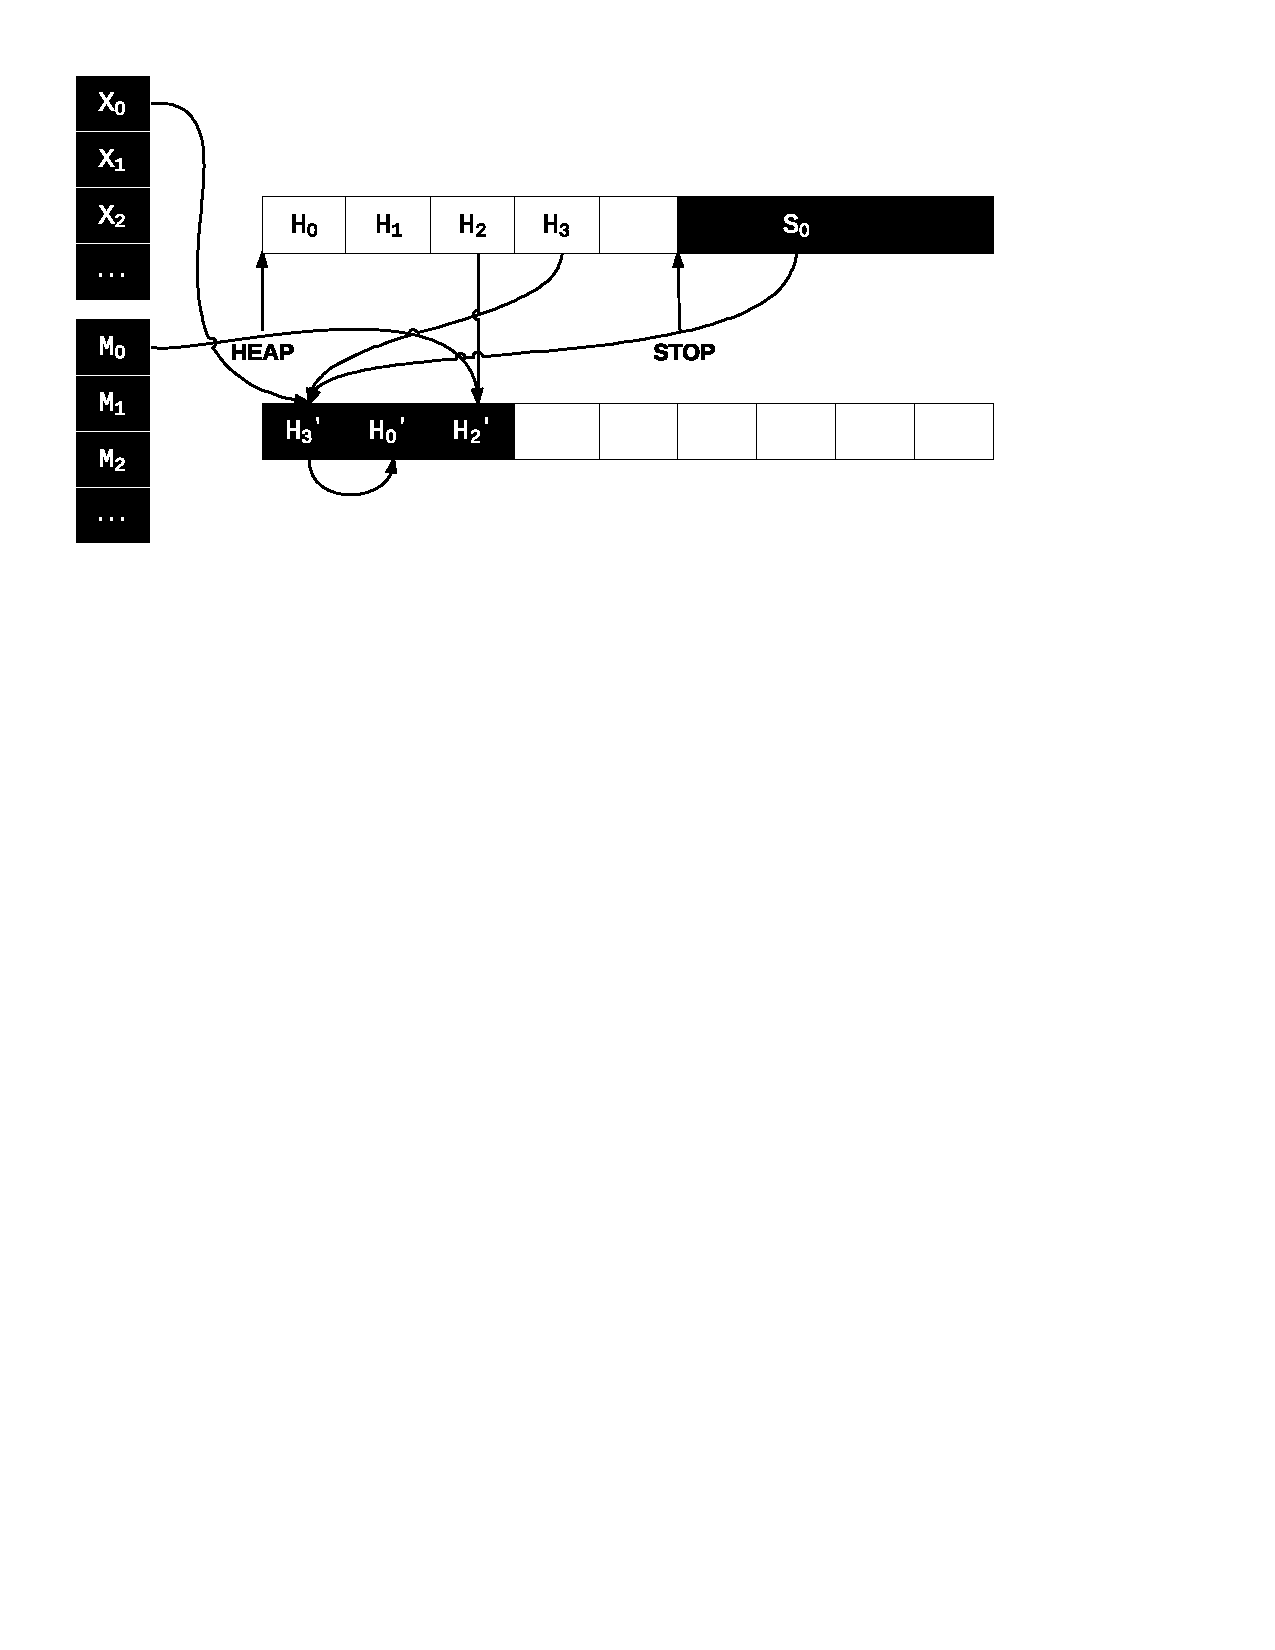
\includegraphics[scale=0.75, clip, trim=10mm 185mm 45mm 10mm]{gc_4}}
\caption{Podmiana wskaźnika do już przeniesionego wyrażenia.}
\label{fig:gc4}
\end{figure}

Przedostatnim krokiem działania algorytmu było skopiowanie stosu procesu, gdyż znajduje się on zawsze w tym samym bloku pamięci co sterta, a więc również zostaje usunięty w trakcie działania \emph{garbage collectora}.
Dokonano także przepisania odpowiednich wskaźników oznaczających początek sterty i stosu procesu (rys. \ref{fig:gc5}).

\begin{figure}[h]
\centerline{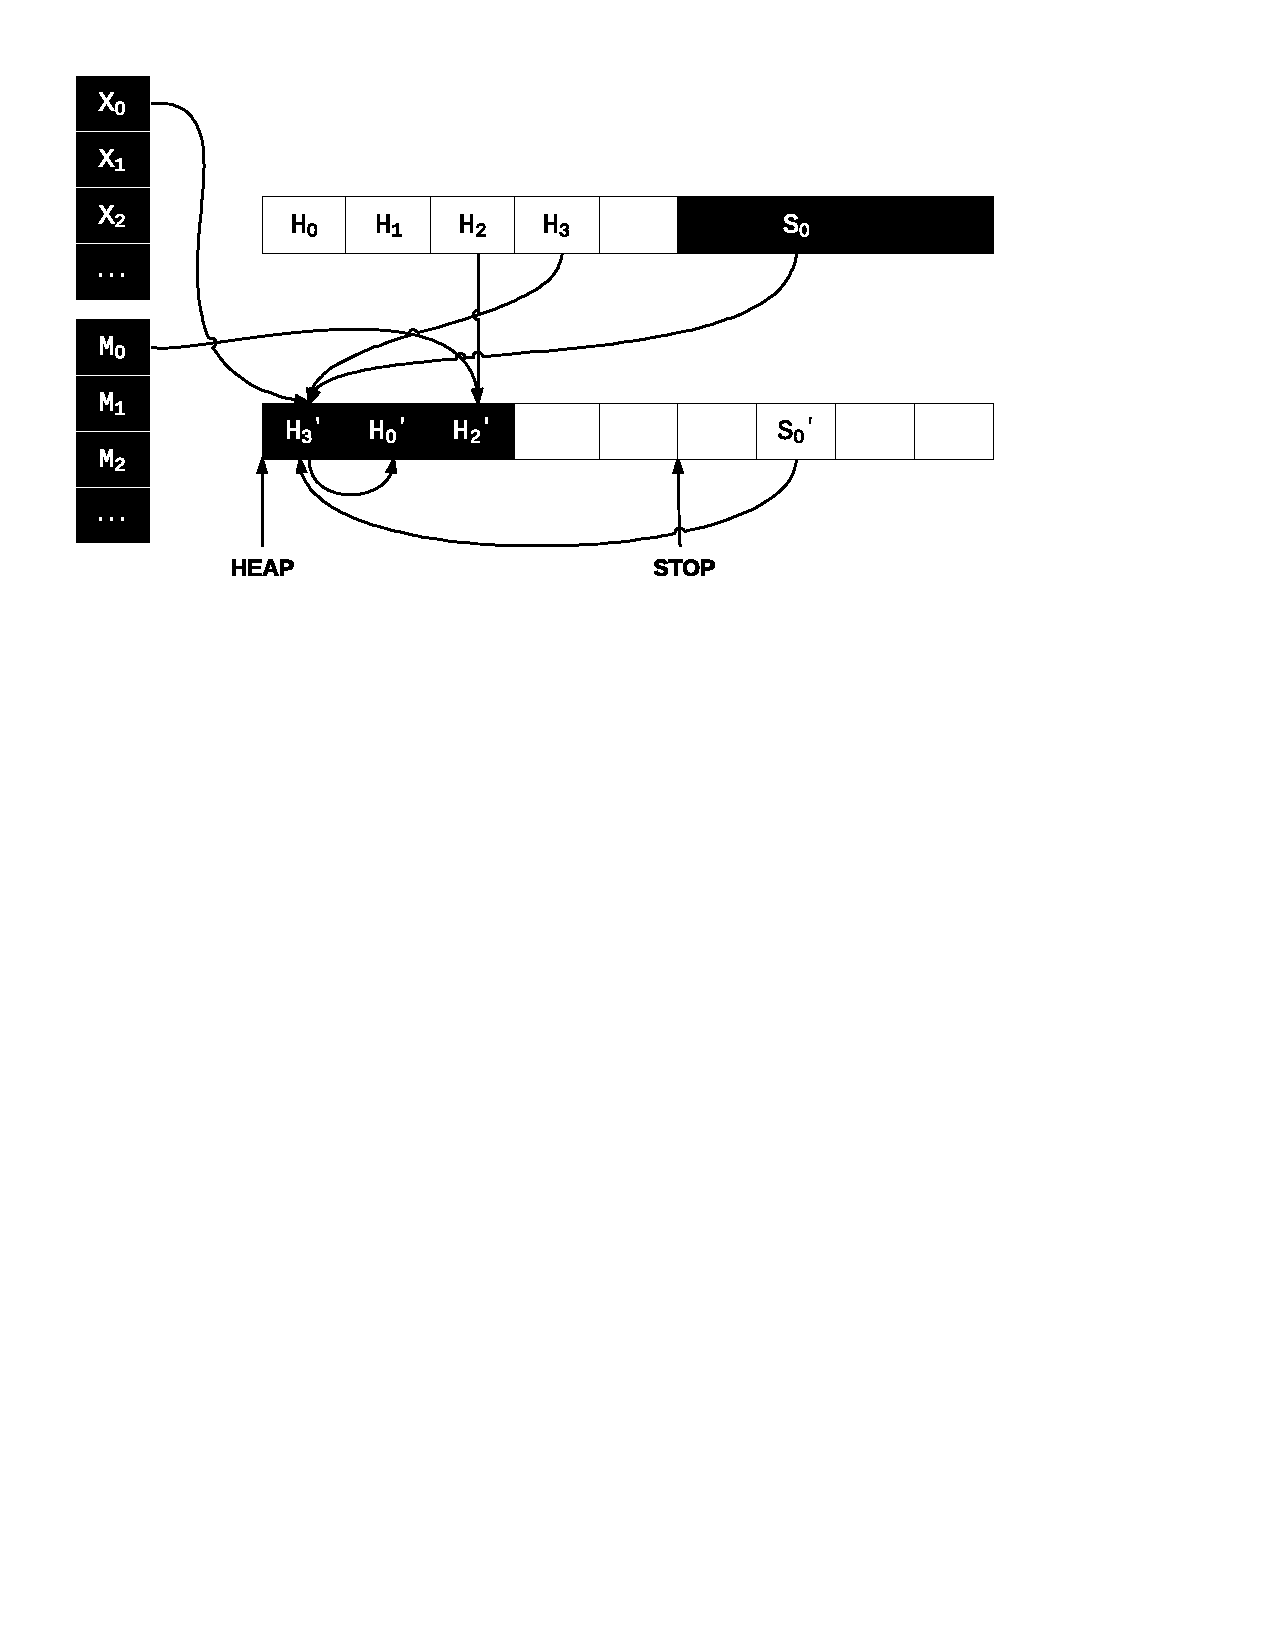
\includegraphics[scale=0.75, clip, trim=10mm 180mm 45mm 10mm]{gc_5}}
\caption{Kopiowanie stosu na nową stertę i przepisanie odpowiednich wskaźników.}
\label{fig:gc5}
\end{figure}

Końcowym krokiem działania algorytmu było zwolnienie dotychczas używanego bloku pamięci. Jak można zauważyć, na nowej stercie nie ma wyrażenia \textbf{H\textsubscript{1}}, które nie było już wykorzystywane w momencie uruchomienia algorytmu (rys. \ref{fig:gc6}).

\begin{figure}[h]
\centerline{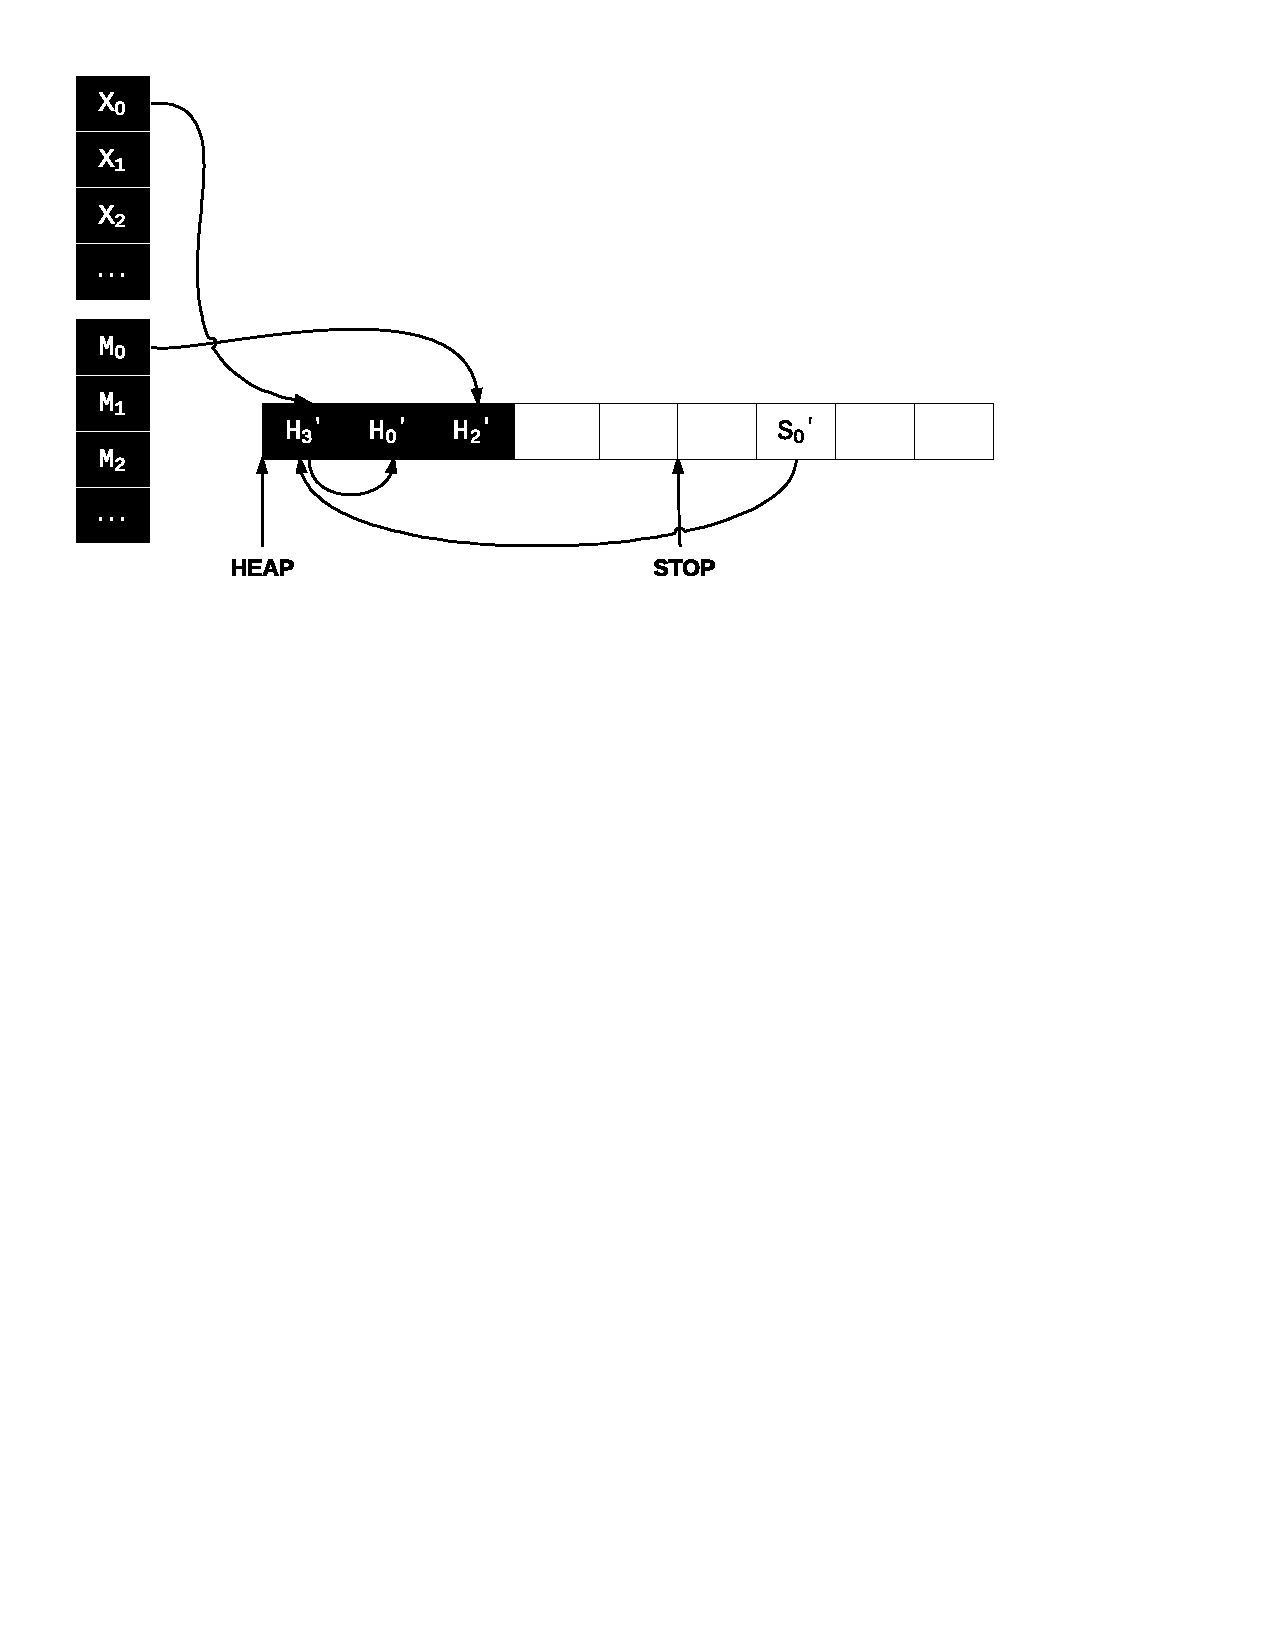
\includegraphics[scale=0.75, clip, trim=10mm 180mm 45mm 10mm]{gc_6}}
\caption{Zwolnienie pamięci zajmowanej przez starą stertę.}
\label{fig:gc6}
\end{figure}

Jeżeli dojdzie do sytuacji, w której po uruchomieniu \emph{garbage collectora} na stercie nie będzie odpowiedniej ilości miejsca dla nowych obiektów, dokonane zostanie rozszerzenie sterty. Polega ono na zaalokowaniu nowego obszaru pamięci, o kolejnym możliwym rozmiarze niż obecny i przeniesieniu stosu oraz wszystkich wyrażeń ze sterty.
W takiej sytuacji konieczne jest również przepisanie referencji obiektów do nowych miejsc w pamięci.
Po zakończeniu tego procesu źródłowa sterta jest zwalniania.

Analogiczną operację wykonuje się w sytuacji, gdy pamięć zajmowana przez nowe obiekty zajmuje co najwyżej pewnien ustalony rozmiar.
W maszynie wirtualnej został on ustalony na połowę rozmiaru starej sterty.
W takiej sytuacji sterta procesu jest zmniejszana do najbliższego wymaganemu rozmiarowi i, podobnie jak w przypadku rozszerzania sterty, zawartość sterty i stos przenoszone są do nowego bloku pamięci.

\subsection{Podejście generacyjne w maszynie BEAM}
\label{sub:gcGeneracje}

Maszyna BEAM w procesie odśmiecania korzysta dodatkowo z podejścia generacyjnego.
Opiera się ono na obserwacji, że większość utworzonych obiektów usuwana jest z pamięci stosunkowo wcześnie, a~obiekty które ,,przetrwały'' przynajmniej jedno uruchomienie \emph{garbage collectora} prawdopodobnie przetrwają i kolejne.
Prowadzi to do podziału obiektów na dwie generacje, którym przypisane są osobne sterty: ,,młodą'' i ,,starą''.
Pierwsza z nich zawiera niedawno utworzone obiekty, które nie zostały poddane jeszcze żadnemu procesowi odśmiecania.
Druga z kolei przechowuje obiekty, które zostały utworzone w pamięci przed przynajmniej jednym uruchomieniem \emph{garbage collectora}.
Odśmiecanie ,,starej'' sterty odbywa się z założenia zdecydowanie rzadziej niż jest to w przypadku obszaru pamięci z nowymi obiektami.
Częstość ta w maszynie wirtualnej BEAM jest parametrem konfigurowalnym przez zmienną środowiskową \texttt{ERL\_FULLSWEEP\_AFTER}, której wartość mówi co ile uruchomień \emph{garbage collectora} na ,,młodej'' generacji obiektów uruchomiony on zostanie również dla ,,starej'' generacji.
Im większa wartość, tym sam proces odśmiecenia trwa zdecydowanie krócej, proces wykorzystuje jednak więcej pamięci.

W maszynie wirtualnej zaimplementowanej w pracy nie została zaimplementowana ta optymalizacja algorytmu odśmiecania. 


%---------------------------------------------------------------------------
\section{Mechanizmy zarządzania czasem}
\label{sec:maszynaTimer}

Moduł opisany w niniejszym podrozdziale został zaimplementowany w pliku źródłowym \texttt{erl\_time.c}.

Język Erlang zapewnia dwie konstrukcje pozwalające na ustawienie przeterminowania po upływie zadanego czasu, po którym przez maszynę wirtualną zostanie wykonana pewna czynność:
\begin{itemize}
\item konstrukcja \texttt{receive ... after ... end} --- zawieszająca wykonywanie się procesu aż do momentu otrzymania wiadomości, kiedy to przeterminowanie zostaje usunięte z listy aktywnych lub do upłynięcia ustalonego czasu w milisekundach, kiedy proces wznawia działanie wykonując najpierw kod w bloku \texttt{after};
\item wywołanie funkcji wbudowanej \texttt{erlang:send\_after/3} --- kolejkującej wysłanie wiadomości do wskazanego procesu po upłynięciu zadanego czasu. Usunięcia tak utworzonego przeterminowania można dokonać poprzez wywołanie innej funkcji wbudowanej \texttt{erlang:cancel\_timer/1}.
\end{itemize}

Wymienione funkcjonalności związane z zarządzeniem przeterminowaniami zostały zaimplementowane w maszynie wirtualnej opisywanej w pracy.

Strukturą danych służącą do zapamiętania aktywnych przeterminowań jest koło czasowe, będące tablicą dwukierunkowych list przeterminowań, o określonej z góry długości. Sposób działania mechanizmu został zaprezentowany na rysunkach od \ref{fig:tiw1} do \ref{fig:tiw3}.

Na rysunku \ref{fig:tiw1} zaprezentowano wygląd struktury w momencie uruchomienia maszyny wirtualnej.
Koło czasowe ma tutaj 128 pól, a rozdzielczość każdego z nich to 1 milisekunda.
Wskaźnik, oznaczony na rysunkach czerwoną strzałką, zapamiętuje aktualne pole koła czasowego.
W momencie aktualizacji czasu wskaźnik ten jest przesuwany o odpowiednią liczbę pól, a w przypadku dojścia do końca tablicy ustawiany jest on ponownie na jej początku.
\begin{figure}[h]
\centerline{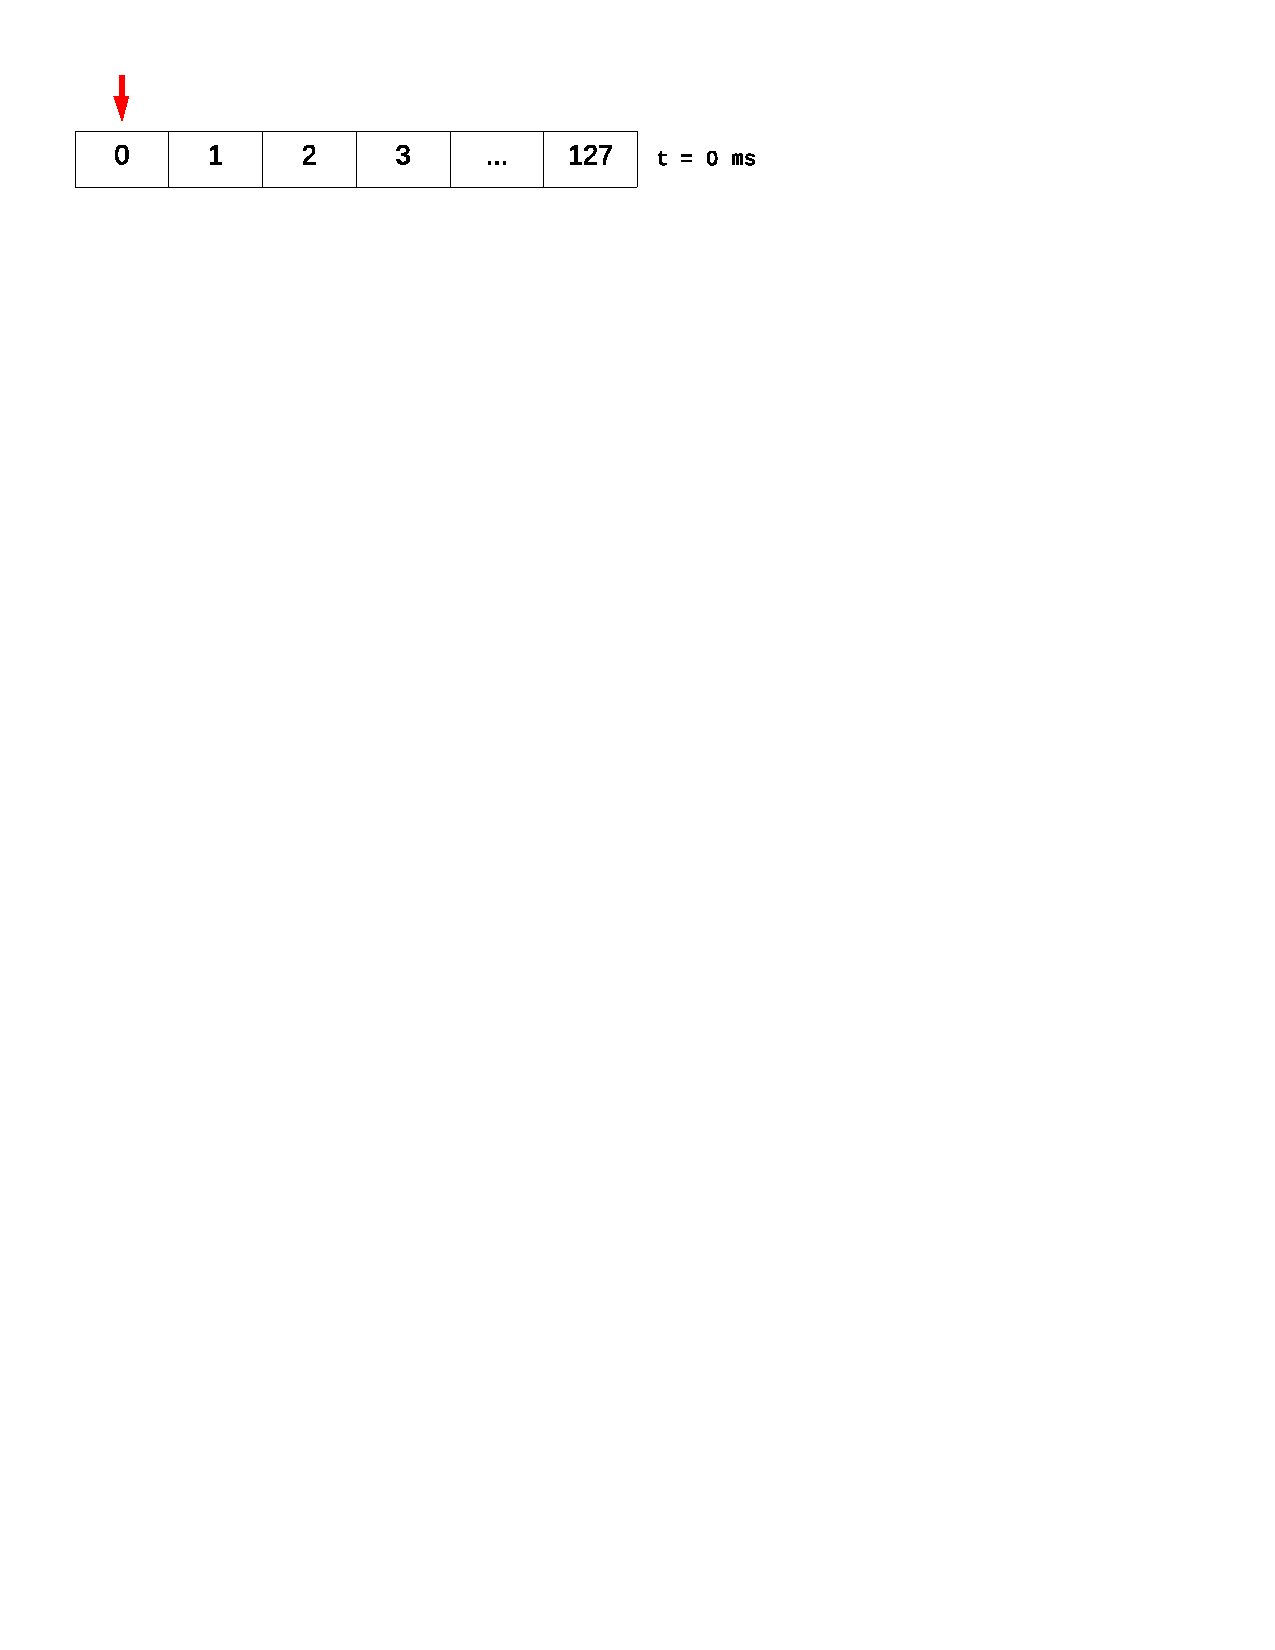
\includegraphics[scale=0.75, clip, trim=10mm 245mm 80mm 10mm]{tiw1}}
\caption{Stan koła czasowego w momencie uruchomienia systemu.}
\label{fig:tiw1}
\end{figure}

Na rys. \ref{fig:tiw2} zaprezentowano wygląd koła czasowego po upływie 2 milisekund od uruchomienia systemu.
W międzyczasie do koła czasowego dodano dwa przeterminowania:
\begin{itemize}
\item do zrealizowania za 1 milisekundę --- ponieważ aktualne pole w kole czasowym to 2, przeterminowanie zostało dodane na pozycji 3 i zostanie zrealizowane przy kolejnej aktualizacji czasu;
\item do zrealizowania za 257 milisekund --- realizacja przeterminowania może nastąpić dopiero po dwukrotnym przejściu wskaźnika przez całe koło czasowe (256 ms) i dojścia do pozycji nr 3~w~tablicy, dlatego w przypadku tego przeterminowania wartość licznika ustawiona została na 2.
\end{itemize}

\begin{figure}[h]
\centerline{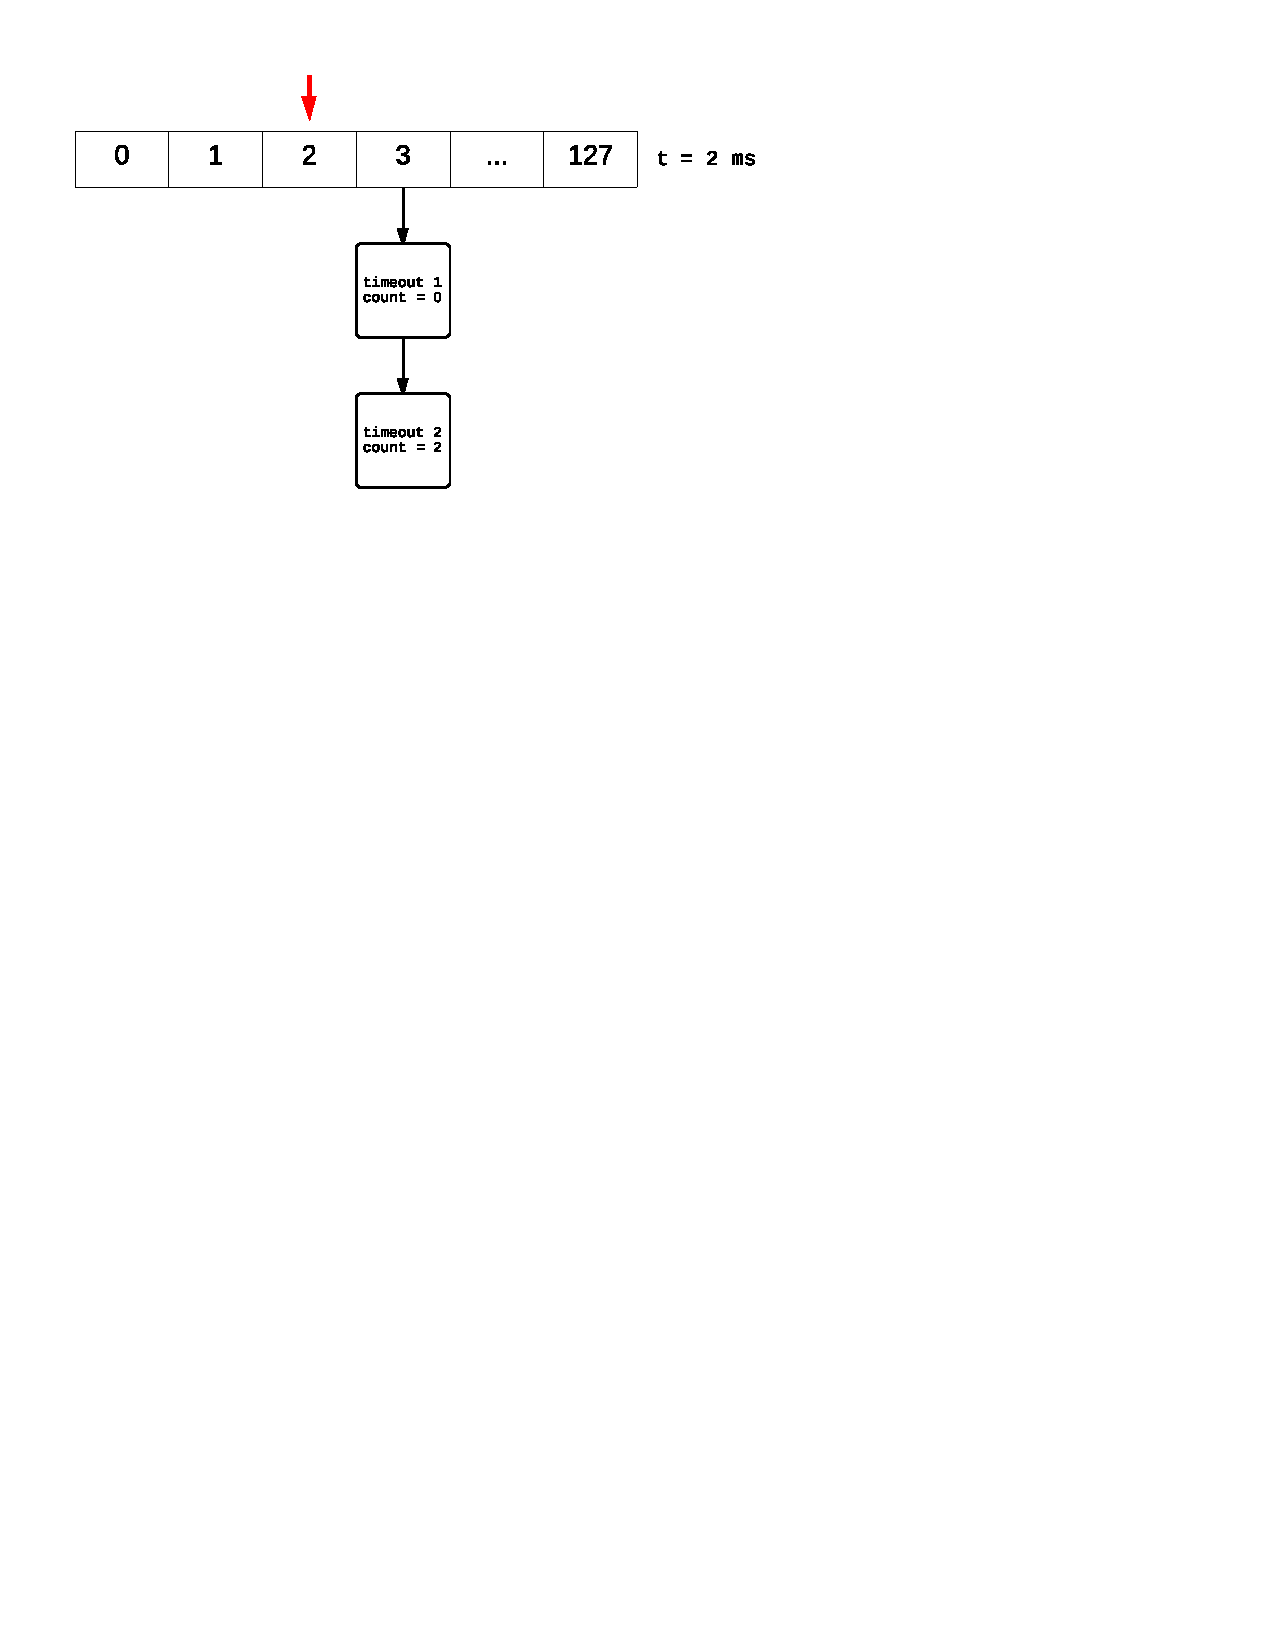
\includegraphics[scale=0.75, clip, trim=10mm 195mm 80mm 10mm]{tiw2}}
\caption{Koło czasowe z dodanymi dwoma przeterminowaniami.}
\label{fig:tiw2}
\end{figure}

Rysunek \ref{fig:tiw3} przedstawia stan koła czasowego w 259. milisekundzie.
Wskaźnik, oznaczony czerwoną strzałką, w porównaniu do stanu zaprezentowanego na poprzednim rysunku wykonał dwa pełne przejścia przez całą tablicę koła czasowego.
Każda aktualizacja czasu (przesunięcie wskaźnika) pociąga za sobą aktualizację przeterminowań na pozycjach mijanych przez wskaźnik.
Jeżeli licznik przeterminowania jest równy zeru oznacza to, że przeterminowanie powinno zostać zrealizowane i usunięte z listy na danej pozycji.
W przeciwnym wypadku, przeterminowanie przeznaczone jest do zrealizowania w którymś z kolejnych przejść wskaźnika przez daną pozycję koła czasowego. Dlatego też licznik danego przeterminowania zostaje zmniejszony o 1.

\begin{figure}[h]
\centerline{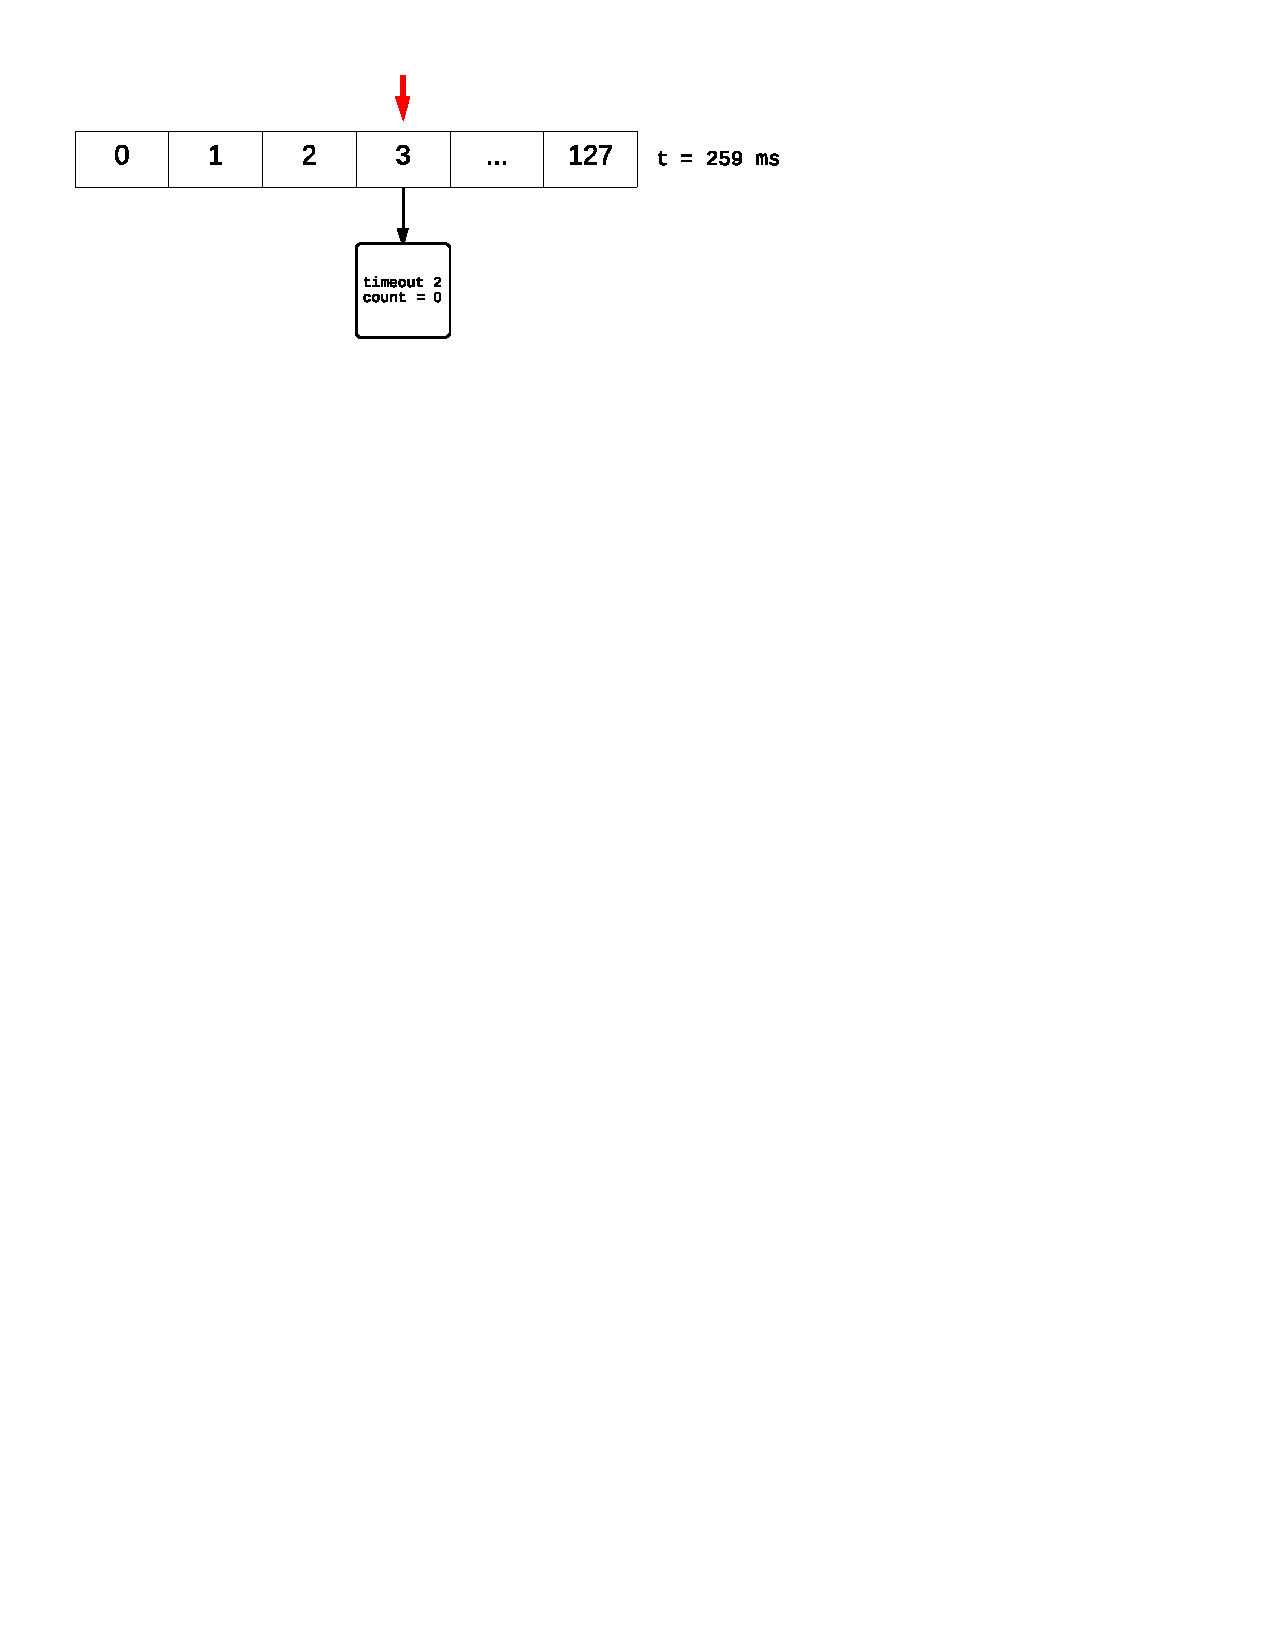
\includegraphics[scale=0.75, clip, trim=10mm 220mm 80mm 10mm]{tiw3}}
\caption{Koło czasowe z jednym przeterminowaniem, które zostanie zrealizowane przy kolejnej aktualizacji czasu.}
\label{fig:tiw3}
\end{figure}

Jedyną różnicą w budowie koła czasowa pomiędzy maszyną zaimplementowaną w pracy a maszyną BEAM jest jej rozmiar.
W maszynie BEAM składa się ona aż z 65536 pozycji.
Rozmiar ten, ze względu na ograniczony rozmiar dostępnej pamięci, w niniejszej maszynie został ograniczony do minimum.

Aspektem różniącym obie maszyny w działaniu mechanizmów zarządzania czasem jest również sposób aktualizacji czasu, a co za tym idzie częstość aktualizacji wskaźnika koła czasowego.
W maszynie wirtualnej BEAM wskaźnik aktualizowany jest na podstawie zegara systemowego pomiędzy wykonywaniem kolejnych procesów z kolejek, a także gdy nie ma w nich żadnych procesów do uruchomienia.
Z~kolei w zaimplementowanej maszynie wirtualnej rola aktualizacji czasu przejęta została przez fizyczny zegar aktualizowany taktowaniem o częstotliwości 1 kHz.
Zegar uruchamia przerwanie w mikrokontrolerze, a kod je obsługujący aktualizuje pozycję wskaźnika koła czasowego i aktualizuje jego stan wraz z~realizacją odpowiednich przeterminowań.
W idealnym przypadku więc pozycja wskaźnika będzie aktualizowana z częstotliwością równą rozdzielczości koła czasowego (co 1 milisekundę), jednak opóźnienia w obsłudze przerwania mogą prowadzić do rzadszej jego aktualizacji.

W niniejszej maszynie wirtualnej została zaimplementowana została także funkcja wbudowana \texttt{erlang:now/0}, różniąca się jednak działaniem od jej odpowiednika w maszynie BEAM tym, że zwraca czas jaki upłynął od momentu uruchomienia systemu, nie zaś od początku 1 stycznia 1970 r.
Czas pozyskiwany jest z, innego niż w przypadku aktualizacji czasu w kole czasowym, fizycznego zegara mikrokontrolera LPC1769, aktualizowanego taktowaniem o częstotliwości 1 MHz.

%---------------------------------------------------------------------------
\section{Podsumowanie różnic z maszyną BEAM}
\label{sec:maszynaPodsumowanie}

Na elementy, z których składa się maszyna wirtualna Erlanga można popatrzeć z punktu widzenia poszczególnych obszarów pamięci przez nią zajmowanych.

Do elementów tych należą:
\begin{itemize}
\item skompilowany kod wykonywalny modułów opisanych w niniejszym rozdziale;
\item tablice: atomów, eksportowanych funkcji, portów i procesów;
\item kolejki procesów i portów, na podstawie których \emph{scheduler} decyduje o wyborze kolejnego procesu do wykonania;
\item uruchomione procesy z informacjami kontrolnymi, kolejkami wiadomości i pamięcią do nich należącą;
\item załadowany kod pośredni modułów, który wykonywany jest w kontekście procesów;
\item globalna sterta, na której umieszczane są stałe wyrażenia pochodzące z plikami z modułów;
\item tablice ETS (\emph{Erlang Term Storage}) stanowiące w maszynie wirtualnej mutowalny obszar pamięci, w postaci bazy danych klucz-wartość;
\item sterta, na której przechowywane są dane typu binarnego, których długość wynosi przynajmniej 64 bajtów. Dane te mogą być współdzielone przez procesy, których liczba przechowywana jest przez licznik referencji, na którego podstawie \emph{garbage collector} zwalnia nieużywane już obszary pamięci.
\end{itemize}

Na rysunku \ref{fig:ertsmemory} zaprezentowany został powyższy podział, z uwzględnieniem elementów które posiada zarówno maszyna BEAM jak i maszyna zaimplementowana w pracy, które zostały oznaczone kolorem czarnym.
Kolorem niebieskim z kolei oznaczone zostały elementy, które nie zostały zaimplementowane w maszynie na system FreeRTOS.
Strzałki na diagramie przedstawiają fakt przechowywania wskaźników na elementy w jednym obszarze pamięci przed drugi.

\begin{figure}[h]
\centerline{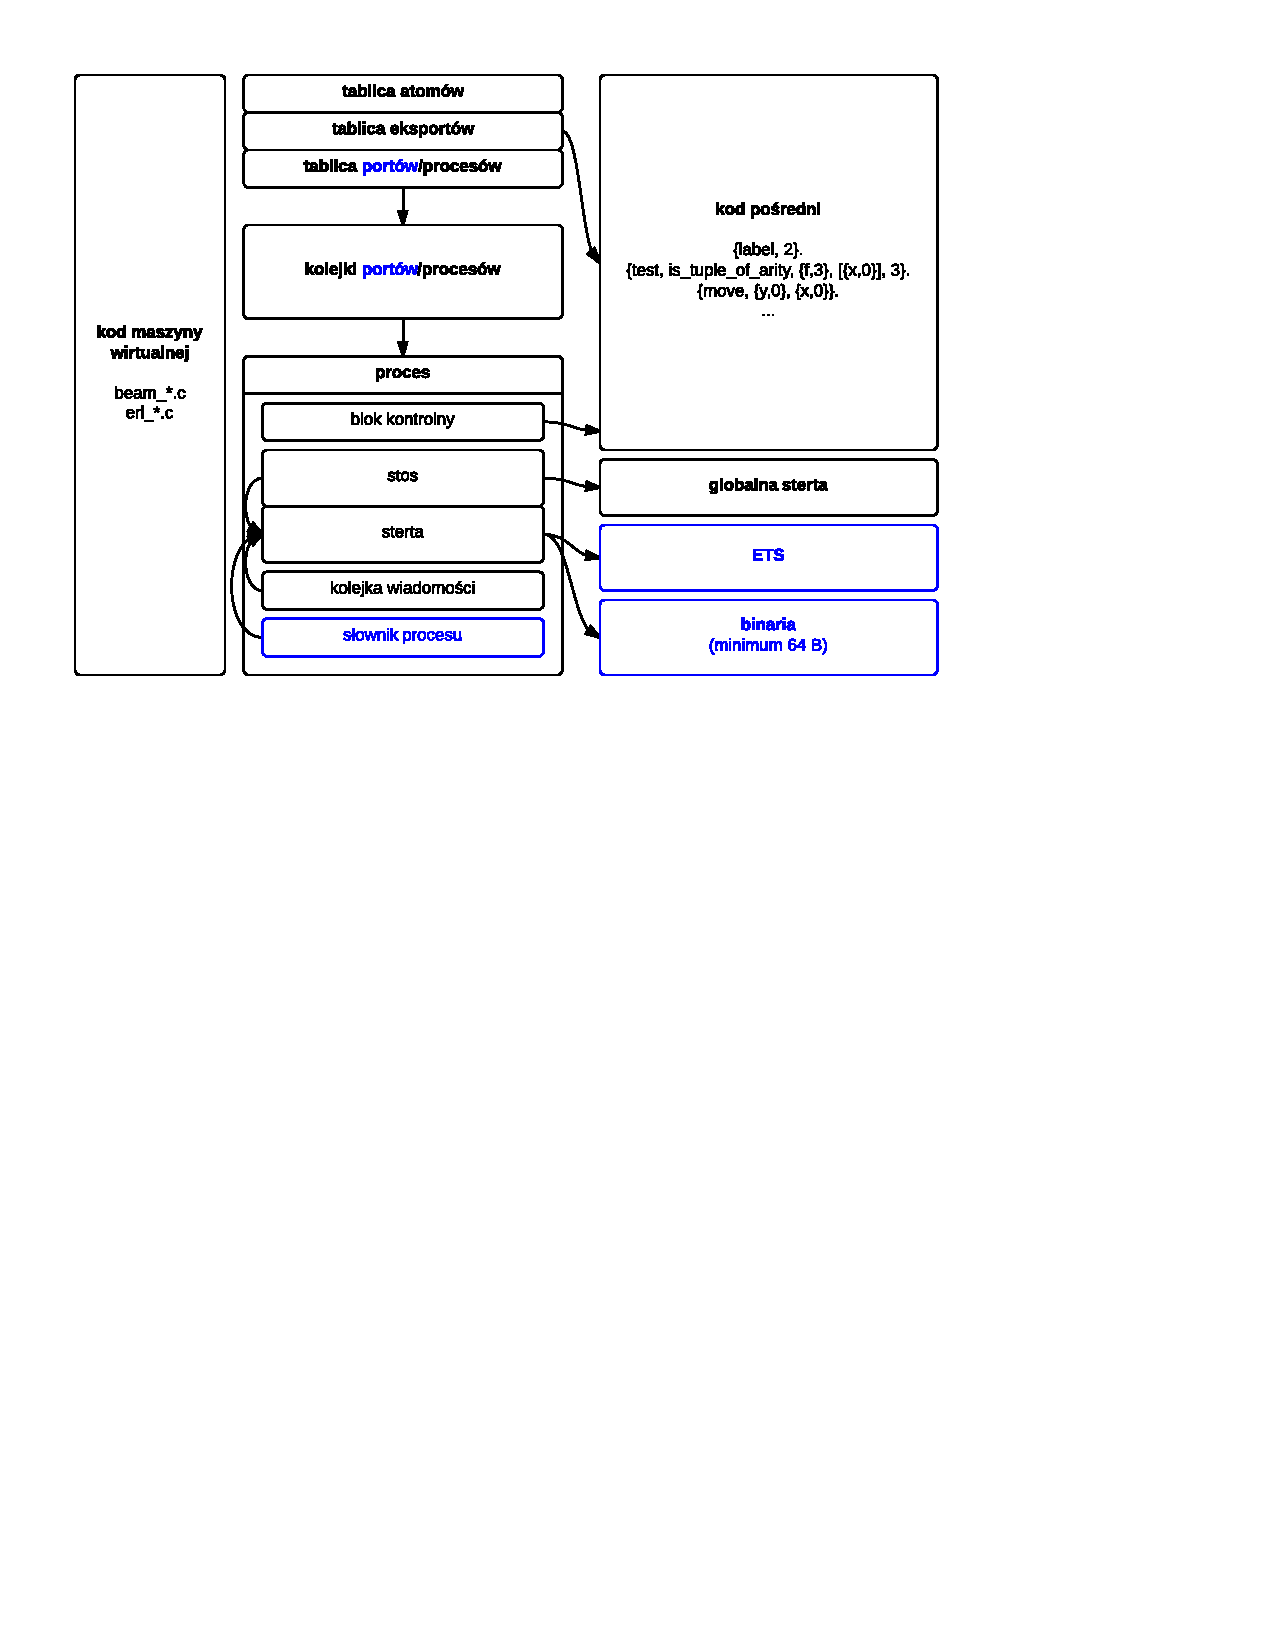
\includegraphics[scale=1, clip, trim=10mm 165mm 55mm 10mm]{erts_memory}}
\caption{Elementy maszyny wirtualnej Erlanga jako obszary pamięci.}
\label{fig:ertsmemory}
\end{figure}

Elementami, które nie zostały zaimplementowane w pracy są: tablice ETS oraz słownik procesu, których użycie nie jest konieczne do implementacji w pełni funkcjonalnych modułów w języku Erlang. Nie pozostały również zaimplementowane sterta binariów oraz tablice i kolejki portów, ze względu na niezaimplementowanie tych typów danych w maszynie.